\documentclass[10pt,aspectratio=169]{beamer}
\usepackage{appendixnumberbeamer}
\usetheme{default}
\usecolortheme{default}
\definecolor{ceruleanblue}{rgb}{0.2,0.2,0.7}
\setbeamertemplate{navigation symbols}{}
\setbeamertemplate{footline}{
  \hfill%
  \usebeamercolor[fg]{page number in head/foot}%
  \usebeamerfont{page number in head/foot}%
  \insertframenumber\,/\,\inserttotalframenumber\kern1em\vskip2pt%
}
\setbeamertemplate{footnote}{%
  \parindent 0em\noindent%
  \raggedright
  \insertfootnotemark\insertfootnotetext
}
\setbeamertemplate{headline}{}
\setbeamercolor{background canvas}{bg=white}
\setbeamercolor{frametitle}{fg=brown!130, bg=white} %titre de chaque frame
\setbeamercolor{enumerate item}{fg=red}
\usepackage[utf8]{inputenc}
\usepackage{amsmath,amssymb}
\usepackage{cancel}
\usepackage{graphicx}
\usepackage{tikz}
\usepackage{tikz-3dplot}
\usetikzlibrary{patterns,calc}
\usepackage{subcaption}
\usepackage{booktabs}
\usepackage[svgnames]{xcolor}
\usepackage[dvipsnames]{xcolor}
\usepackage{eurosym}
\usepackage{animate}
\usepackage{media9}
\usepackage{hyperref}
\usepackage{pstool}
  \usepackage{cancel}
\definecolor{darkgray}{RGB}{64,64,64}% Custom colors - minimalist grayscale palette
\definecolor{lightgray}{RGB}{128,128,128}
\definecolor{mediumgray}{RGB}{96,96,96}
\definecolor{lightblue}{RGB}{173,216,230}
\definecolor{Magenta4}{HTML}{8f008f}
\definecolor{Red4}{HTML}{8f0000}
\definecolor{Cyan4}{HTML}{008f8f}
\definecolor{Blue4}{HTML}{00008f}
\definecolor{blue4}{HTML}{00008f}
\definecolor{red4}{HTML}{8f0000}
\definecolor{cyan4}{HTML}{008f8f}
\definecolor{green4}{HTML}{008f00}
\definecolor{green2}{HTML}{00ff00}
\usepackage{lmodern}% Font settings for clean look
\usefonttheme{structurebold}
\setbeamerfont{title}{size=\Large, series=\bfseries}
\setbeamerfont{frametitle}{size=\large, series=\bfseries}
\setbeamerfont{framesubtitle}{size=\normalsize, series=\mdseries}

\setbeamerfont{section in toc}{series=\bfseries} % Table of contents formatting
\setbeamerfont{subsection in toc}{series=\bfseries}
\setbeamercolor{section in toc}{fg=ceruleanblue}
\setbeamercolor{subsection in toc}{fg=gray}
\setbeamercolor{block title}{bg=ceruleanblue, fg=ceruleanblue!20}% Clean block and theorem environments
\setbeamercolor{block body}{bg=ceruleanblue, fg=ceruleanblue!20}
\setbeamertemplate{blocks}[rounded][shadow=false]
\setbeamertemplate{itemize items}[circle] % Clean itemize bullets
\setbeamercolor{itemize item}{fg=ceruleanblue}
\setbeamercolor{itemize subitem}{fg=ceruleanblue}
\everymath{\displaystyle} % Mathematical formatting
\definecolor{darkRed}{rgb}{0.55,0,0}
\definecolor{darkGreen}{rgb}{0,0.39,0}
\definecolor{darkBlue}{rgb}{0.16,0.32,0.75}
\definecolor{Red}{rgb}{0.8,0,0}
\definecolor{Green}{rgb}{0,0.6,0}
\usetikzlibrary{decorations.pathmorphing,arrows.meta,calc,patterns,3d}

% Theorem environments (Beamer already defines theorem, lemma, corollary, definition, etc.)
\newtheorem{proposition}{Proposition}

% Theorem block colors
\setbeamercolor{block title}{bg=ceruleanblue!20, fg=ceruleanblue!80!black}
\setbeamercolor{block body}{bg=ceruleanblue!5, fg=black}

% Automatic outline at each section and subsection
% \AtBeginSection[]{
%   \begin{frame}{Outline}
%     \tableofcontents[currentsection,hideothersubsections]
%   \end{frame}
% }

% \AtBeginSubsection[]{
%   \begin{frame}{Outline}
%     \tableofcontents[currentsection,currentsubsection]
%   \end{frame}
% }

%%%%%%%%%%%%%%%%%%%%%%%%%%% title
\title[Embedded Convex Optimization for PMSM Control]{Embedded Convex Optimization for Control of Synchronous machines}

\subtitle{PhD Defense}

\author[H. Houmsi]{Hiba HOUMSI}

\institute[INSA Lyon]{
    Laboratoire Ampère\\
    INSA Lyon\\
    \vspace{0.2cm}
    \textbf{Supervisors:}
    Paolo Massioni, Federico Bribiesca-Argomedo, Romain Delpoux
}
\date{\today}
% Logo (adjust path as needed)\logo{\includegraphics[height=1cm]{logo_insa.png}}

\begin{document}

% ========================================
% Introduction and Problem Statement
% ========================================
%%%%%%%%%%%%%%%%%%% Frame de garde
\begin{frame}[plain]
    \begin{center}
        \vspace{1cm}
        \textcolor{ceruleanblue}{\Large \bfseries Embedded Convex Optimization for Control of Synchronous machines} \\
        \vspace{0.8cm}
        {\normalsize Hiba HOUMSI}\\
        \vspace{0.3cm}
        {\textbf{\textcolor{brown!130}{Supervisors:}} Paolo Massioni, Federico Bribiesca-Argomedo, Romain Delpoux}\\
        \vspace{0.5cm}
        {\small
        \textbf{\textcolor{brown!130}{Jury Committee:}}\\
        \vspace{0.2cm}
        \begin{tabular}{@{}llll@{}}
            \textbf{Examiner:} & Delphine Riu & Professor & Grenoble INP-Ense3 \\
            \textbf{Reviewers:} & Giorgio Valmorbida & Professor & CentraleSupélec \\
                               & Václav Šmídl &  Professor &  CTU Prague \\
            \textbf{Invited:} & Lubin Kerhuel & PhD Engineer & Microchip, inc.
        \end{tabular}
        }\\
        \vspace{0.6cm}
        %{\footnotesize Ampère laboratory, INSA Lyon, France}
        %\vspace{0.2cm}
        {\footnotesize PhD Defense, \today}

        \vspace{0.1cm}
        \begin{figure}[htbp]
        \begin{center}
        \href{http://www.ampere-lab.fr/}{
\includegraphics[height = 1cm]{pictures/logo/logoAMPERE}}
        \href{https://www.insa-lyon.fr/}{
\includegraphics[height = 1cm]{pictures/logo/INSA}}
        
\includegraphics[height=1cm]{pictures/logo/CNRS}
        
\includegraphics[height=1cm]{pictures/logo/UDL}
        
\includegraphics[height=1cm]{pictures/logo/Centrale}
        
\includegraphics[height=1cm]{pictures/logo/Lyon1}
        \end{center}
        \end{figure}
    \end{center}
\end{frame}
%%%%%%%%%%%%%%%%%%% Frame de Venn diagram
\section{Problem statement}
\begin{frame}{Problem Statement}{The embedded approach}
         \only<1->{
            Implement \textcolor{Red}{advanced control laws synthesis} on \textcolor{ceruleanblue}{low-cost hardware} to drive \textcolor{Green}{real-world systems}.
     }
     \vspace{-0.5cm}
     \begin{figure}
        %\centering
        \begin{tikzpicture}[scale= 0.8]
        \coordinate (origin) at (0,0);
        \only<2->{% Green circle - appears from slide 4 onwards
            \draw [Green, line width=0.8mm](0,-1.5) circle (2);
            \node at (0,-2.5) {\textcolor{Green}{\shortstack{Control \\ Application}}};
            %\node at (-5,-3) {\includegraphics[width=2.5cm]{pictures/PMSM.eps}};
            \node at (-5,-5) {\shortstack{Permanent magnet \\ synchronous machines}};
            \draw [Green, line width=0.6mm, dashed, ->] (-0,-3.5) to[bend left=15] (-3,-5);
        }
        \only<3->{% Red circle - persistent from slide 2 onwards
            \draw [red,line width=0.8mm] (-1.3,0) circle (2);
            \node at (-1.8,1) {\textcolor{red}{\shortstack{Convex \\ Optimization}}};
           % \node at (-5.5,2) {\includegraphics[width=2.5cm]{pictures/Robust_control_law.eps}};
            %\node at (-8.5,2) {\includegraphics[width=2.5cm]{pictures/Robust_control_law.eps}};
            %\node at (-5.5,0) {\shortstack{Feedback \\ control}};
            %\node at (-8.5,0) {\shortstack{Trajectory \\ generation}};
            \node at (-5.5,2) {\shortstack{Feedback \\ control}};
            \node at (-8.5,2) {\shortstack{Trajectory \\ generation}};
            \draw [red, line width=0.6mm, dashed, ->] (-2,2) to[bend right=15] (-4,2);
        }
        \only<4->{% Blue circle - appears from slide 3 onwards
            \draw [ceruleanblue,line width=0.8mm] (1.3,0) circle (2);
            \node at (1.7,1) {\textcolor{ceruleanblue}{\shortstack{Embedded \\ systems}}};
            %\node at (5,1) {\includegraphics[width=2.5cm]{pictures/muC.eps}};
            %\node at (5,-1) {\shortstack{Microcontrollers \\ DSP}};
            \node at (5,1) {\shortstack{Microcontrollers \\ DSP \\ $\sim 5 \$ $/unit}};
            \draw [ceruleanblue, line width=0.6mm, dashed, ->] (2,2) to[bend left=15] (4.5,2);
        }
        \path[use as bounding box] (-10,-5) rectangle (10,3);% Invisible bounding box to maintain consistent tikzpicture size
        \end{tikzpicture}
     \end{figure}
\end{frame}

%%%%%%%%%%%%%%%%%%% Control engineer approach Hybrid offline online approach 
 \begin{frame}{Problem Statement}{The embedded approach}
    \begin{center}
    \only<1>{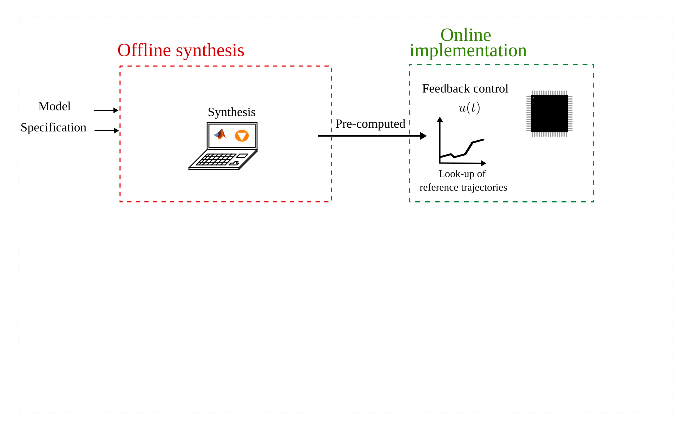
\includegraphics[trim={0cm 0cm 0cm 0cm},clip,width=0.9\framewidth]{pictures/online_offline1.eps}
    }
    %\only<2>{\includegraphics[trim={0cm 0cm 0cm 0cm},clip,width=0.9\framewidth]{pictures/online_offline_ink_trajec1.eps}
    %}
    \only<2>{
    \vspace{-0.3cm}    
    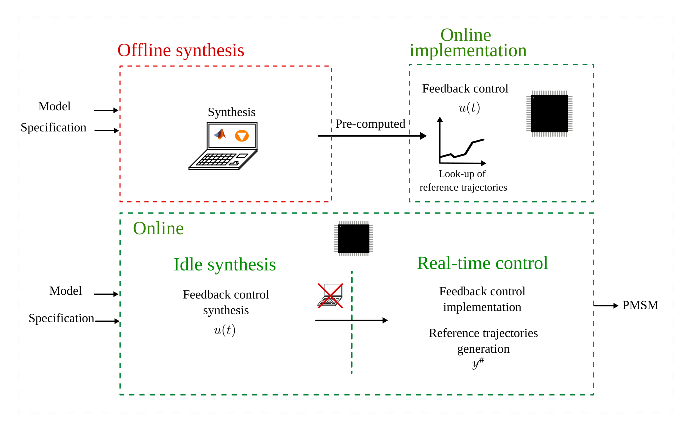
\includegraphics[trim={0cm 0cm 0cm 0cm},clip,width=0.9\framewidth]{pictures/online_offline2.eps}
    }
    \end{center}
 \end{frame}
%%%%%%%%%%%%%%%%%%% Frame PMSM is widely used
\begin{frame}{Problem Statement}
    Permanent Magnet Synchronous Motors (PMSM)
    \begin{center}
        Widely used in industry
    \end{center}
\vspace{-.5cm}
\begin{columns}[t]
    \begin{column}{0.33\textwidth}
    \begin{center}
        \only<1->{
        Automotive\\
        \vspace{.5cm}
        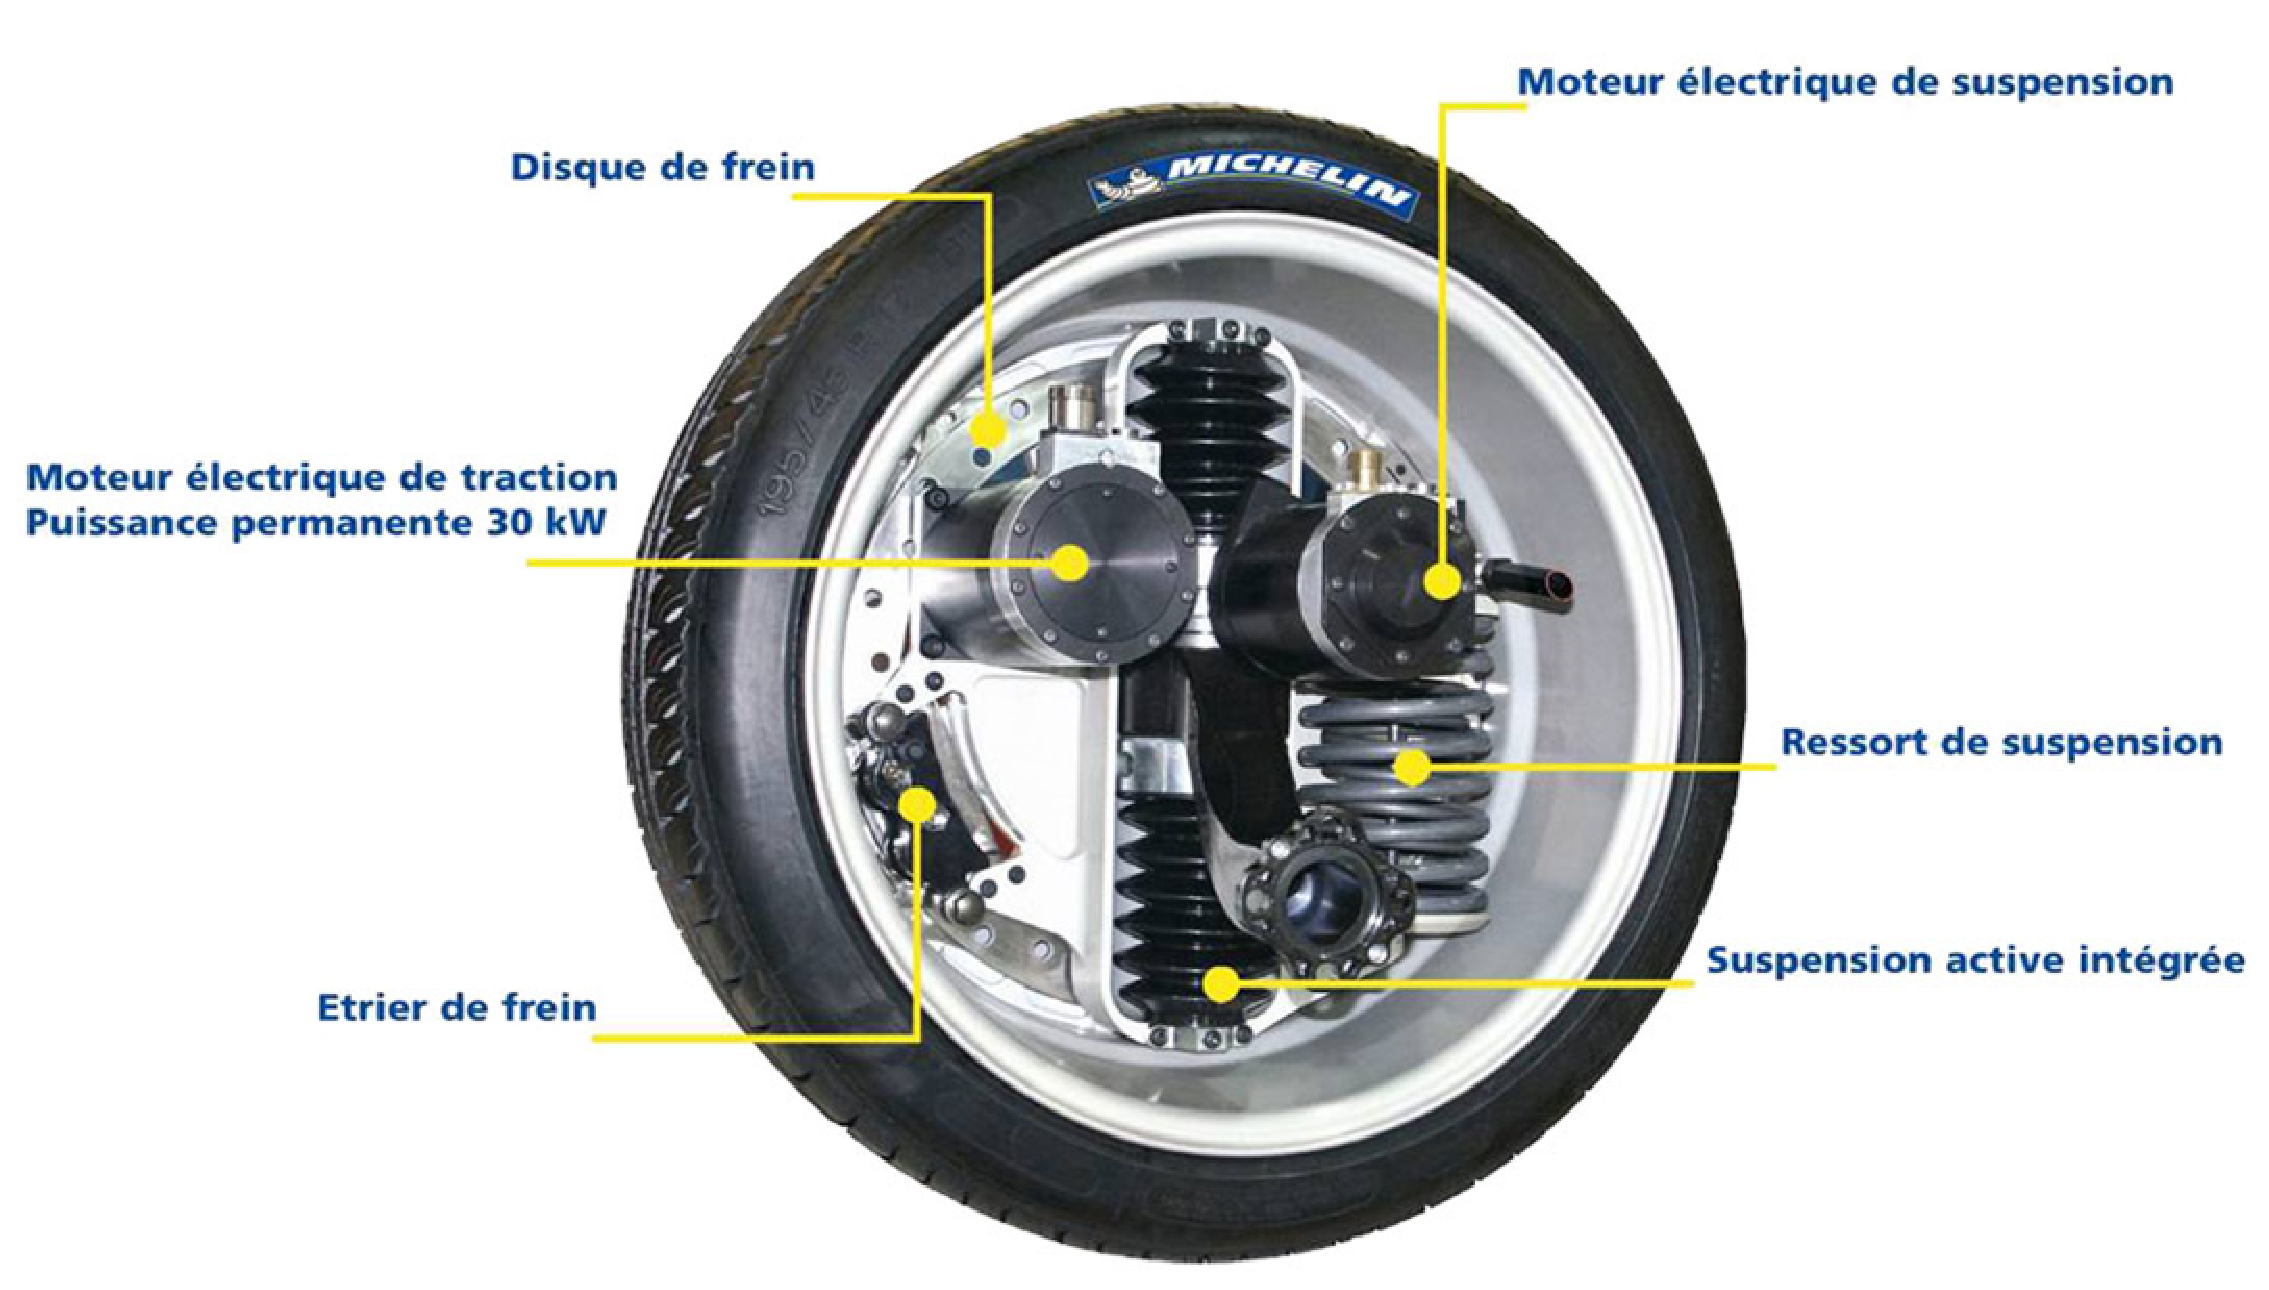
\includegraphics[width=0.8\textwidth]{pictures/Michelin.eps}
        }
    \end{center}
    \end{column}
%
    \begin{column}{0.33\textwidth}
    \begin{center}
    \only<2->{
        Robotics\\
        \vspace{.5cm}
        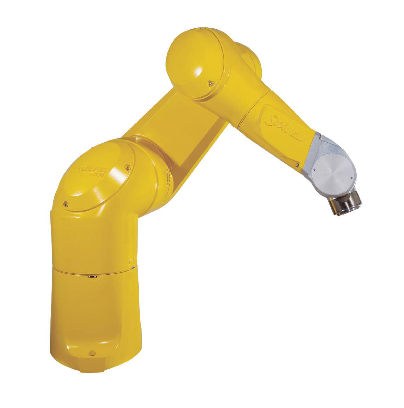
\includegraphics[width=0.8\textwidth]{pictures/TX90.eps}
    }
    \end{center}
\end{column}
    \begin{column}{0.33\textwidth}
        \begin{center}
        \only<3->{
        Power generation
        \vspace{.5cm}
        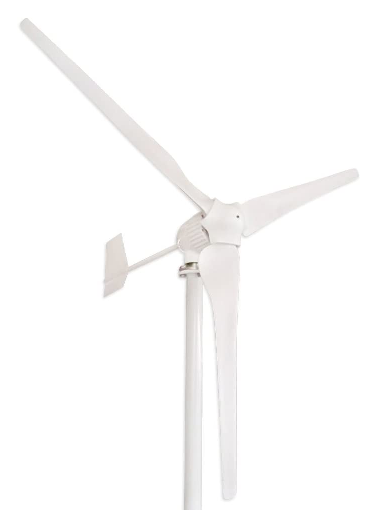
\includegraphics[width=.5\textwidth]{pictures/eolienne.eps}}
        \end{center}
    \end{column}
\end{columns}
    \only<4>{
    \vspace{.5cm}
    \alert{Goal: control torque and speed, while minimizing losses, taking into consideration the physical limitations.}}
\end{frame}
%%%%%%%%%%%%%%%%%%% Frame Park and Clarke transformations
\begin{frame}{Problem statement}{Simple representation of 3-phase PMSM}
    \begin{figure}
    \begin{tikzpicture}[scale=1.2]
    \tikzstyle{axis}=[thick,->]    % Styles
    \tikzstyle{coil}=[decoration={aspect=0.2, segment length=1mm, amplitude=3mm,coil},decorate,opacity=0.9]
    \tikzstyle{vector}=[->, thick]
    % ========== LEFT PART: 3D PMSM Representation ==========
    \only<1->{
    \begin{scope}[shift={(1,1)},scale=0.8]
        \coordinate (O) at (0,0);% Origin
        \fill[gray!40,rotate=50] (-0.8,-0.25) rectangle (0.8,0.25); % Draw rotor (rectangular, uniform light gray)
        \draw[thick,rotate=50] (-0.8,-0.25) rectangle (0.8,0.25);
        % Phase a axis (horizontal, towards front)
        \begin{scope}
            \draw[axis,black!70] (O) -- (0:2.8);
            \node at (0:3.0) {$a$};
            % Coil
            \draw[coil] (0:1.8) -- (0:2.2);
            % Voltage arrow (parallel to coil, 0.5cm offset below)
            \draw[vector,red] (1.8,-0.5) -- (2.2,-0.5) node[midway,below] {$v_{a}$};
            % Current arrow (on axis, closer to center)
            \draw[vector,blue] (1.1,0) -- (1.5,0) node[midway,below] {$i_{a}$};
        \end{scope}
        % Phase b axis (120 degrees)
        \begin{scope}[rotate=120]
            \draw[axis,black!70] (O) -- (0:2.8);
            \node at (0:3.0) {$b$};
            % Coil
            \draw[coil] (0:1.8) -- (0:2.2);
            % Voltage arrow (parallel to coil, 0.5cm offset below)
            \draw[vector,red] (1.8,-0.5) -- (2.2,-0.5) node[midway,right] {$v_{b}$};
            % Current arrow (on axis, closer to center)
            \draw[vector,blue] (1.1,0) -- (1.5,0) node[midway,below] {$i_{b}$};
        \end{scope}
        % Phase c axis (240 degrees)
        \begin{scope}[rotate=240]
            \draw[axis,black!70] (O) -- (0:2.8);
            \node at (0:3.0) {$c$};
            % Coil
            \draw[coil] (0:1.8) -- (0:2.2);
            % Voltage arrow (parallel to coil, 0.5cm offset below)
            \draw[vector,red] (1.8,-0.5) -- (2.2,-0.5) node[midway,left] {$v_{c}$};
            % Current arrow (on axis, closer to center)
            \draw[vector,blue] (1.1,0) -- (1.5,0) node[midway,right] {$i_{c}$};
        \end{scope}
        % Rotor angle theta_r
        \draw[thick,red] (O) -- (50:1.3) ; % node[midway,above,sloped,inner sep=1pt] {$\mathcal{N}$};
        \draw[-{Stealth[length=2mm]},thick,blue] (0.6,0) arc (0:50:0.6);
        \node at (25:1.2) {$\theta_r$};
        % Rotation indication
        \draw[-{Stealth[length=3mm]},thick,gray,dashed] (20:1.8) arc (20:80:1.8);
    \end{scope}
    % Label for left part
    \node at (1,-1.5) {\textbf{Static 3-coordinate system}};
    }
    % ========== RIGHT PART: d-q Frame Detail ==========
    \only<2>{
    \begin{scope}[shift={(7,1)},scale=0.8]
        \coordinate (C) at (0,0);
        % d-q axes
        \draw[axis,black!70,thick] (C) -- (50:3.5) node[anchor=south west] {$d$};
        \draw[axis,black!70,thick] (C) -- (140:3.5) node[anchor=south east] {$q$};
        % Angle theta_r from horizontal to d-axis
        \draw[-{Stealth[length=2mm]},thick,red] (0.8,0) arc (0:50:0.8);
        \node at (25:1.1) {$\theta_r$};
        \draw[axis,gray,dashed] (C) -- (0:1.2);
        \node at (0:1.4) {$\alpha$};
        % d-axis circuit (along d-axis)
        \begin{scope}[rotate=50]
            % Inductance L_d (coil)
            \draw[coil] (1.5,0) -- (2.0,0);
            \node at (1.75,0.5) {\small $L_d$};
            % Current arrow (on axis, further from coil)
            \draw[vector,blue] (2.1,0) -- (2.5,0) node[midway,below] {\small $i_d$};
            % Voltage arrow (at same height as coil)
            \draw[vector,red] (1.6,-0.5) -- (2,-0.5) node[midway,below=3pt] {\small $v_d$};
        \end{scope}
        % q-axis circuit (along q-axis)
        \begin{scope}[rotate=140]
            % Inductance L_q (coil)
            \draw[coil] (1.5,0) -- (2.0,0);
            \node at (1.75,0.5) {\small $L_q$};
            % Current arrow (on axis, further from coil)
            \draw[vector,blue] (2.6,0) -- (3.0,0) node[midway,below] {\small $i_q$};
            % Voltage arrow (at same height as coil)
            \draw[vector,red] (1.5,-0.5) -- (2 ,-0.5) node[midway,above=3pt] {\small $v_q$};
        \end{scope}
        % Rotor flux indication
        \draw[-{Stealth[length=3mm]},thick,red] (C) -- (50:1.2);
        \node[red] at (75:0.5) {$\phi_f$};
    \end{scope}
    % Label for right part
    \node at (7,-1.5) {\textbf{Rotating 2-coordinate system}};

    % Curved arrow showing transformation between the two systems
    \draw[-{Stealth[length=3mm]},thick,blue!70,line width=1.2pt]
        (3.2,0.31) to[out=-20,in=-160] (4.8,0.31);
    \node[align=center,fill=white,inner sep=2pt] at (4,-0.51)
        {\small \textbf{Park \& Clarke}\\ \small \textbf{transformation}};
    }
\end{tikzpicture}
    \end{figure}
\end{frame}
%%%%%%%%%%%%%%%%%%%%%%%%%%%%% Model of  the PMSM

\begin{frame}{Model of the PMSM}
    The nonlinear model of the system in the dq frame can  be represented as
 \begin{eqnarray*}
         L_d \frac{di_d}{dt} &=& v_d - Ri_d \textcolor{red}{+p L_q\omega i_q}, \\
         L_q\frac{di_q}{dt} &=& v_q -Ri_q \textcolor{red}{-pL_d\omega i_d} -p \phi_f\omega, \\
         J\frac{d\omega}{dt} &=&  \tau_{em}  - f\omega \textcolor{violet}{-\tau_l}.
     \end{eqnarray*}
     \pause
The system is subject to physical constraints:
    \begin{eqnarray*}
        & i_{dq}^\top i_{dq} - i_{max}^2 \leqslant 0, \\
        & v_{dq}^\top v_{dq} - v_{max}^2 \leqslant 0 ,  \\
        &\tau_{em} = \frac{3}{2}p \big( \phi_f +  (L_d - L_q) i_d \big) i_q.
    \end{eqnarray*}
\end{frame}
\begin{frame}{Problem statement}{System constraint}
    \begin{columns}
    \begin{column}{0.4\framewidth}
         \begin{eqnarray*}
            &\tikz[remember picture,baseline=(idqeq.base)]{\node[inner sep=0pt](idqeq){$i_{dq}^\top i_{dq} - i_{max}^2 \leqslant 0$};}\\
            \only<1-2>{&  \tikz[remember picture,baseline=(vdqeq.base)]{\node[inner sep=0pt](vdqeq){$v_{dq}^\top v_{dq} - v_{max}^2\leqslant 0$,};} \\}
            \only<3-4>{&  \tikz[remember picture,baseline=(vdqeq.base)]{\node[inner sep=0pt,align=center](vdqeq){$\textcolor{orange}{A(\omega)} i_d^2 + \textcolor{orange}{B(\omega)}i_di_q + \textcolor{orange}{C(\omega)}i_q^2+$ \\ $ \textcolor{orange}{D(\omega)}i_d + \textcolor{orange}{E(\omega)}i_q + \textcolor{orange}{F(\omega)} \leqslant 0$};} \\}
            \only<1-3>{& \tikz[remember picture,baseline=(taueq.base)]{\node[inner sep=0pt](taueq){$\tau_{em} - \frac{3}{2}p \big( \phi_f +  (L_d - L_q) i_d \big) i_q= 0.$}; }}
            \only<4>{& \tikz[remember picture,baseline=(taueq.base)]{\node[inner sep=0pt](taueq){$\textcolor{red}{\tau_{em}} - \frac{3}{2}p \big( \phi_f +  (L_d - L_q) i_d \big) i_q= 0.$}; }}
         \end{eqnarray*}
         \tikz[remember picture,overlay] {
            \only<1>{\draw[dashed,very thick,rounded corners,blue] ([xshift=-0.1cm,yshift=0.2cm]idqeq.north west) rectangle ([xshift=0.1cm,yshift=-0.08cm]idqeq.south east);}
            \only<2>{\draw[dashed,very thick,rounded corners,orange] ([xshift=-0.1cm,yshift=0.1cm]vdqeq.north west) rectangle ([xshift=0.1cm,yshift=-0.08cm]vdqeq.south east);}
            \only<3>{\draw[dashed,very thick,rounded corners,orange] ([xshift=-0.1cm,yshift=0.1cm]vdqeq.north west) rectangle ([xshift=0.1cm,yshift=-0.08cm]vdqeq.south east);}
            \only<4>{\draw[dashed,very thick,rounded corners,red] ([xshift=-0.1cm,yshift=0.1cm]taueq.north west) rectangle ([xshift=0.1cm,yshift=-0.08cm]taueq.south east);}
            }
    \end{column}
    \begin{column}{0.6\framewidth}
    \centering
     \only<1>{
        Current constraint in the $i_{dq}$ frame
        \centering
        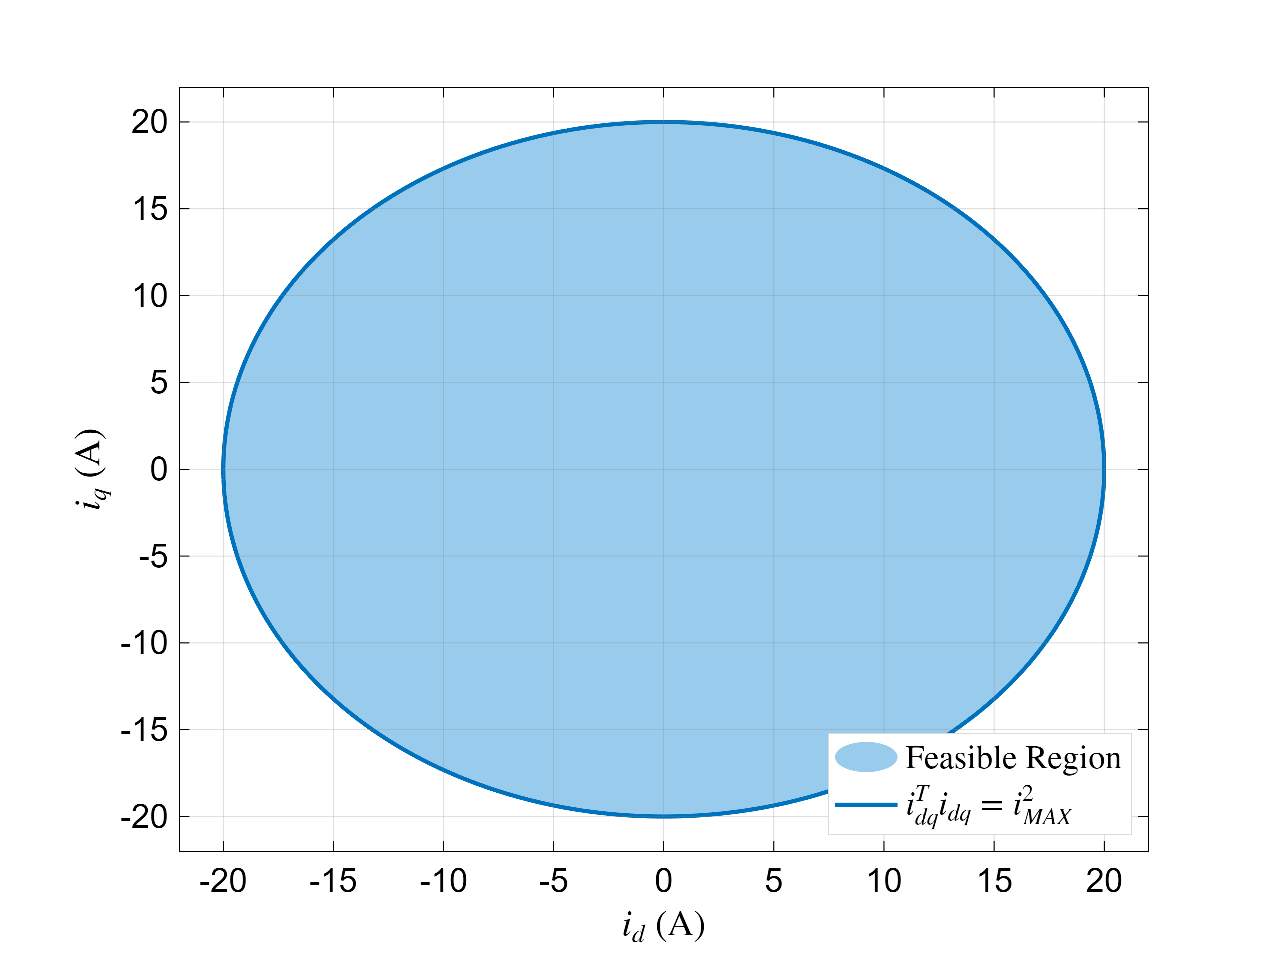
\includegraphics[width=7cm]{pictures/current_constraint_cost.eps}
     }
     \only<2>{
        Voltage constraint in the $i_{dq}$ frame
         \begin{eqnarray*}
            \cancel{L_d \frac{di_d}{dt}} &=& v_d - Ri_d +p L_q\omega i_q = 0, \\
            \cancel{L_q\frac{di_q}{dt}} &=& v_q -Ri_q -pL_d\omega i_d -p \phi_f\omega = 0,
       \end{eqnarray*}
     }
     \only<3>{
     \begin{center}
         \animategraphics[loop,controls,width=1\textwidth]{10}{eps_frames_voltage_animation_filled/frame_}{000}{040}
      \end{center}
     }
     \only<4>{
        Torque constraint in the $i_{dq}$ frame
      \begin{center}
          \animategraphics[loop,controls,width=1\textwidth]{10}{eps_frames_voltage_animation_torque/frame_}{000}{040}
      \end{center}
     }
    \end{column}
    \end{columns}
\end{frame}

\begin{frame}{Problem statement}%{To sum up}
\only<1->{
    \vspace{-0.3cm}
    \textbf{Goals:}
   % \vspace{0.2cm}
    %\hspace{+0.2cm}
    \begin{enumerate}
        \item[\textcolor{Cyan4}{\textbf{Part 1:}}] \textcolor{Cyan4}{Optimal currents $i_d^\#$, $i_q^\#$ to produce desired torque $\tau_{em}$ and speed $\omega$ }
        \only<2->{\item[\textcolor{Magenta4}{\textbf{Part  2:}}] \textcolor{Magenta4}{Embedded closed-loop control synthesis}}
        \only<3->{\item[\textcolor{blue}{\textbf{Part 3:}}] \textcolor{blue}{New control apporachs}}
    \end{enumerate}
}
\vspace{+0.1cm}
\begin{columns}[T]
    \begin{column}{0.5\textwidth}
        \tikz[remember picture,baseline=(optimalprob.base)]{\node[inner sep=5pt,align=left](optimalprob){\begin{minipage}{\textwidth}
        \textbf{\textcolor{Cyan4}{Part1: Optimal references}}
      \begin{center}
          \animategraphics[loop,autoplay,width=0.7\textwidth]{10}{eps_frames_voltage_animation_torque/frame_}{000}{040}
      \end{center}
        \only<1->{\small Output: $i_d^{\#}(\omega, \tau_{em})$, $i_q^{\#}(\omega, \tau_{em})$}
        \end{minipage}};}
        \tikz[remember picture,overlay] {
            \only<1>{\draw[dashed,very thick,rounded corners,Cyan4] ([xshift=-0.1cm,yshift=0.2cm]optimalprob.north west) rectangle ([xshift=0.1cm,yshift=-0.08cm]optimalprob.south east);}
        }
    \end{column}
    \begin{column}{0.5\textwidth}
    \only<2->{
        \tikz[remember picture,baseline=(controlprob.base)]{\node[inner sep=5pt,align=left](controlprob){\begin{minipage}{\textwidth}
        \textbf{\textcolor{Magenta4}{Part 2: Embedded closed-loop control synthesis}}
        
    %      \begin{eqnarray*}
    %      L_d \frac{di_d}{dt} &=& v_d - Ri_d +p L_q\omega i_q, \\
    %      L_q\frac{di_q}{dt} &=& v_q -Ri_q -pL_d\omega i_d -p \phi_f\omega, \\
    %      J\frac{d\omega}{dt} &=& \tau_{em}  -f\omega -\tau_l.
    %  \end{eqnarray*}
        \vspace{0.3cm} \textbf{Find} $u(t) = Kx(t)$ such that:
        \begin{itemize}
            \item Tracks $i_d^\#$, $i_q^\#$ trajectories
            \item Stable, easy-to-tune
            \item minimise the energy consumption
        \end{itemize}
        \end{minipage}};}
        \tikz[remember picture,overlay] {
            \only<2>{\draw[dashed,very thick,rounded corners,Magenta4] ([xshift=-0.1cm,yshift=0.2cm]controlprob.north west) rectangle ([xshift=0.1cm,yshift=-0.08cm]controlprob.south east);}
        }}
            \only<3->{
                \vspace{+0.3cm}
        \tikz[remember picture,baseline=(controlprob2.base)]{\node[inner sep=5pt,align=left](controlprob2){\begin{minipage}{\textwidth}
        \textbf{\textcolor{blue}{Part 3: Other closed-loop control strategies}}
        
    %      \begin{eqnarray*}
    %      L_d \frac{di_d}{dt} &=& v_d - Ri_d +p L_q\omega i_q, \\
    %      L_q\frac{di_q}{dt} &=& v_q -Ri_q -pL_d\omega i_d -p \phi_f\omega, \\
    %      J\frac{d\omega}{dt} &=& \tau_{em}  -f\omega -\tau_l.
    %  \end{eqnarray*}
        \vspace{+0.3cm}\textbf{Find} $u(t) = K(x(t))$ such that:
        \begin{itemize}
            \item Robust to measurement noise
            \item Robust to parametric uncertainty
        \end{itemize}
        \end{minipage}};}
        \tikz[remember picture,overlay] {
            \only<3>{\draw[dashed,very thick,rounded corners,blue] ([xshift=-0.1cm,yshift=0.2cm]controlprob2.north west) rectangle ([xshift=0.1cm,yshift=-0.08cm]controlprob2.south east);}
        }}
    \end{column}
\end{columns}
% Big frame encompassing both Problem 1 and 2 to show they are embedded in DSP
\tikz[remember picture,overlay] {
    \only<4>{
        \draw[dashed,ultra thick,rounded corners,red] ([xshift=0cm,yshift=0cm]optimalprob.north west) rectangle ([xshift=0cm,yshift=-0.5cm]optimalprob.south -| controlprob.east);
        \node[red,anchor=south east,font=\small\bfseries] at ([xshift=-0.1cm,yshift=-0.5cm]optimalprob.south -| controlprob.east) {Embedded};
    }
}
\only<3>{
\vspace{0.3cm}
\begin{center}
\tikz[remember picture,baseline=(embedprob.base)]{\node[inner sep=8pt,align=center](embedprob){%
\textbf{\textcolor{red}{Embedded}} Embedded implementation on \textcolor{red}{microcontrollers/DSP} ($\sim 5\$$/unit)};}
\tikz[remember picture,overlay] {
    \draw[dashed,very thick,rounded corners,red] ([xshift=0cm,yshift=0cm]embedprob.north west) rectangle ([xshift=0.1cm,yshift=-0.08cm]embedprob.south east);
}
\end{center}
}
\end{frame}

\begin{frame}{Outline}
    %%% loi de commande en boucle fermee
    %    \vspace{-0.3cm}
    \textbf{Objectives:}
    \vspace{0.2cm}
    \begin{enumerate}
        \item[\textcolor{Cyan4}{\textbf{ Part 1:}}] \textcolor{Cyan4}{\textbf{Optimal currents $i_d^\#$, $i_q^\#$ to produce desired torque $\tau_{em}$ and speed $\omega$ ?}}
        \item[\textcolor{Magenta4}{\textbf{Part 2:}}] \textcolor{Magenta4}{\textbf{Embedded closed-loop control synthesis}}
        \item[\textcolor{Blue4}{\textbf{Part 3:}}] \textcolor{Blue4}{\textbf{New control apporachs}}
    \end{enumerate}
        \begin{figure}
            \begin{center}
                \def\textsize{.8}
                \psfrag{Algo}[c][c][1]{\color{Blue4}Control}
                \psfrag{Control}[c][c][1]{\color{Blue4}Control}
                \psfrag{iabc}[c][c][\textsize]{\color{Blue4}$i_{abc}$}
                \psfrag{idq}[c][c][\textsize]{\color{Blue4}$i_{dq}$}
                \psfrag{vabcr}[c][c][\textsize]{\color{Blue4}$v_{abc}^\#$}
                \psfrag{vdqr}[c][c][\textsize]{\color{Blue4}$v_{dq}^\#$}
                \psfrag{dq}[c][c][.5]{\color{Blue4}${dq}$}
                \psfrag{abc}[c][c][.5]{\color{Blue4}${abc}\quad$}
                \psfrag{S}[c][c][\textsize]{\color{Blue4}$S_{abc}$}
                \psfrag{MLI}[c][c][\textsize]{\color{Blue4}Mod}
                \psfrag{ParkInv}[c][c][.5]{}
                \psfrag{Park}[c][c][.5]{}
                \psfrag{TS1}[l][c][.6]{\color{Blue4}Higher priority $\approx20$kHz}
                % Reference generation (cyan) - lower priority optimization
                \psfrag{Vr}[c][c][\textsize]{\color{Cyan4}$\rho^\#$}
                \psfrag{ref}[c][c][\textsize]{\color{Cyan4}$\omega^\#$}
                \psfrag{ref2}[c][c][\textsize]{\color{Cyan4}$i_d^\#$}
                \psfrag{ref3}[c][c][\textsize]{\color{Cyan4}$\omega^\#$}
                \psfrag{ref4}[c][c][\textsize]{\color{Cyan4}$i_q$}
                \psfrag{ref5}[c][c][\textsize]{\color{Magenta4} Specification}
                \psfrag{ref6}[c][c][\textsize]{\color{Magenta4} Model}
                \psfrag{Reference}[c][c][\textsize]{\color{Cyan4}Trajectory}
                \psfrag{calculation}[c][c][\textsize]{\color{Cyan4}generation}
                \psfrag{TS2}[l][c][.6]{\color{Cyan4}Lower priority $\approx1$kHz}
                % Embedded synthesis (magenta) - idle task
                \psfrag{Emb}[c][c][\textsize]{\color{Magenta4}Embedded}
                \psfrag{Synt}[c][c][\textsize]{\color{Magenta4}synthesis}
                \psfrag{K}[c][c][\textsize]{\color{Magenta4}K}
                \psfrag{TS3}[l][c][.6]{\color{Magenta4}Idle task}
                % Physical system (red) - PMSM and measurements
                \psfrag{Onduleur}[c][c][\textsize]{\color{Red4}Invert}
                \psfrag{PMSM}[c][c][\textsize]{\color{Red4}PMSM}
                \psfrag{V}[c][c][\textsize]{\color{Red4}$v_{abc}$}
                \psfrag{th}[c][c][\textsize]{\color{Red4}$\theta$}
                \psfrag{w}[c][c][\textsize]{\color{Red4}$\omega$}
                \psfrag{thm}[c][c][\textsize]{\color{Red4}$\theta$}
                \psfrag{wm}[c][c][\textsize]{\color{Red4}$\omega$}
                \psfrag{Embedded}[l][c][.7]{\color{red}Embedded code}
                \begin{tikzpicture}[remember picture]
                     \node[inner sep=0pt] (diagram) {\includegraphics[width = .9\textwidth]{pictures/AdvancedControl.eps}};
            %         % Arrow pointing to center of Control block (Problem 2 - Blue)
            %         \draw[->,ultra thick,blue] ([xshift=0cm,yshift=-2.8cm]diagram.center) -- ([xshift=0cm,yshift=-0.2cm]diagram.center) node[midway,right,font=\small\bfseries] {Problem 2};
            %         % Arrow pointing to center-bottom of Reference calculation block (Problem 1 - Cyan)
            %         \draw[->,ultra thick,Cyan4] ([xshift=-3cm,yshift=-2.8cm]diagram.center) -- ([xshift=-3cm,yshift=-0.8cm]diagram.center) node[midway,right,font=\small\bfseries] {Problem 1};
            %         % Arrow pointing to center-top of Embedded synthesis block (Problem 3 - Magenta)
            %         \draw[->,ultra thick,Magenta4] ([xshift=-3cm,yshift=2.8cm]diagram.center) -- ([xshift=-3cm,yshift=1.5cm]diagram.center) node[midway,right,font=\small\bfseries] {Problem 3};
                 \end{tikzpicture}
            \end{center}
        \label{fig:AdvancedControlForElectricalMotor}
        \end{figure}
\end{frame}

\begin{frame}{Outline}
    %%% outline generation de trajectoire
        \textbf{Objectives:}
    \vspace{0.2cm}
    \begin{enumerate}
        \item[\textcolor{Cyan4}{\textbf{Part 1:}}] \textcolor{Cyan4}{\textbf{Optimal currents $i_d^\#$, $i_q^\#$ to produce desired torque $\tau_{em}$ and speed $\omega$ ?}}
        \item[\textcolor{gray}{\textbf{Part 2:}}] \textcolor{gray}{\textbf{Embedded closed-loop control synthesis}}
        \item[\textcolor{gray}{\textbf{Part 3:}}] \textcolor{gray}{\textbf{New control approaches}}
    \end{enumerate}
        \begin{figure}
            \begin{center}
                \def\textsize{.8}
                \psfrag{Algo}[c][c][1]{\color{Blue4}Control}
                \psfrag{Control}[c][c][1]{\color{gray}Control}
                \psfrag{iabc}[c][c][\textsize]{\color{Blue4}$i_{abc}$}
                \psfrag{idq}[c][c][\textsize]{\color{Blue4}$i_{dq}$}
                \psfrag{vabcr}[c][c][\textsize]{\color{Blue4}$v_{abc}^\#$}
                \psfrag{vdqr}[c][c][\textsize]{\color{Blue4}$v_{dq}^\#$}
                \psfrag{dq}[c][c][.5]{\color{Blue4}${dq}$}
                \psfrag{abc}[c][c][.5]{\color{Blue4}${abc}\quad$}
                \psfrag{S}[c][c][\textsize]{\color{Blue4}$S_{abc}$}
                \psfrag{MLI}[c][c][\textsize]{\color{Blue4}Mod}
                \psfrag{ParkInv}[c][c][.5]{}
                \psfrag{Park}[c][c][.5]{}
                \psfrag{TS1}[l][c][.6]{\color{Blue4}Higher priority $\approx20$kHz}
                % Reference generation (cyan) - lower priority optimization
                \psfrag{Vr}[c][c][\textsize]{\color{Cyan4}$\rho^\#$}
                \psfrag{ref}[c][c][\textsize]{\color{Cyan4}$\omega^\#$}
                \psfrag{ref2}[c][c][\textsize]{\color{Cyan4}$i_d^\#$}
                \psfrag{ref3}[c][c][\textsize]{\color{Cyan4}$\omega^\#$}
                \psfrag{ref4}[c][c][\textsize]{\color{Cyan4}$i_q$}
                \psfrag{ref5}[c][c][\textsize]{\color{gray} Specification}
                \psfrag{ref6}[c][c][\textsize]{\color{gray} Model}
                \psfrag{Reference}[c][c][\textsize]{\color{Cyan4}Trajectory}
                \psfrag{calculation}[c][c][\textsize]{\color{Cyan4}generation}
                \psfrag{TS2}[l][c][.6]{\color{Cyan4}Lower priority $\approx1$kHz}
                % Embedded synthesis (magenta) - idle task
                \psfrag{Emb}[c][c][\textsize]{\color{gray}Embedded}
                \psfrag{Synt}[c][c][\textsize]{\color{gray}synthesis}
                \psfrag{K}[c][c][\textsize]{\color{gray}K}
                \psfrag{TS3}[l][c][.6]{\color{Magenta4}Idle task}
                % Physical system (red) - PMSM and measurements
                \psfrag{Onduleur}[c][c][\textsize]{\color{Red4}Invert}
                \psfrag{PMSM}[c][c][\textsize]{\color{Red4}PMSM}
                \psfrag{V}[c][c][\textsize]{\color{Red4}$v_{abc}$}
                \psfrag{th}[c][c][\textsize]{\color{Red4}$\theta$}
                \psfrag{w}[c][c][\textsize]{\color{Red4}$\omega$}
                \psfrag{thm}[c][c][\textsize]{\color{Red4}$\theta$}
                \psfrag{wm}[c][c][\textsize]{\color{Red4}$\omega$}
                \psfrag{Embedded}[l][c][.7]{\color{red}Embedded code}
                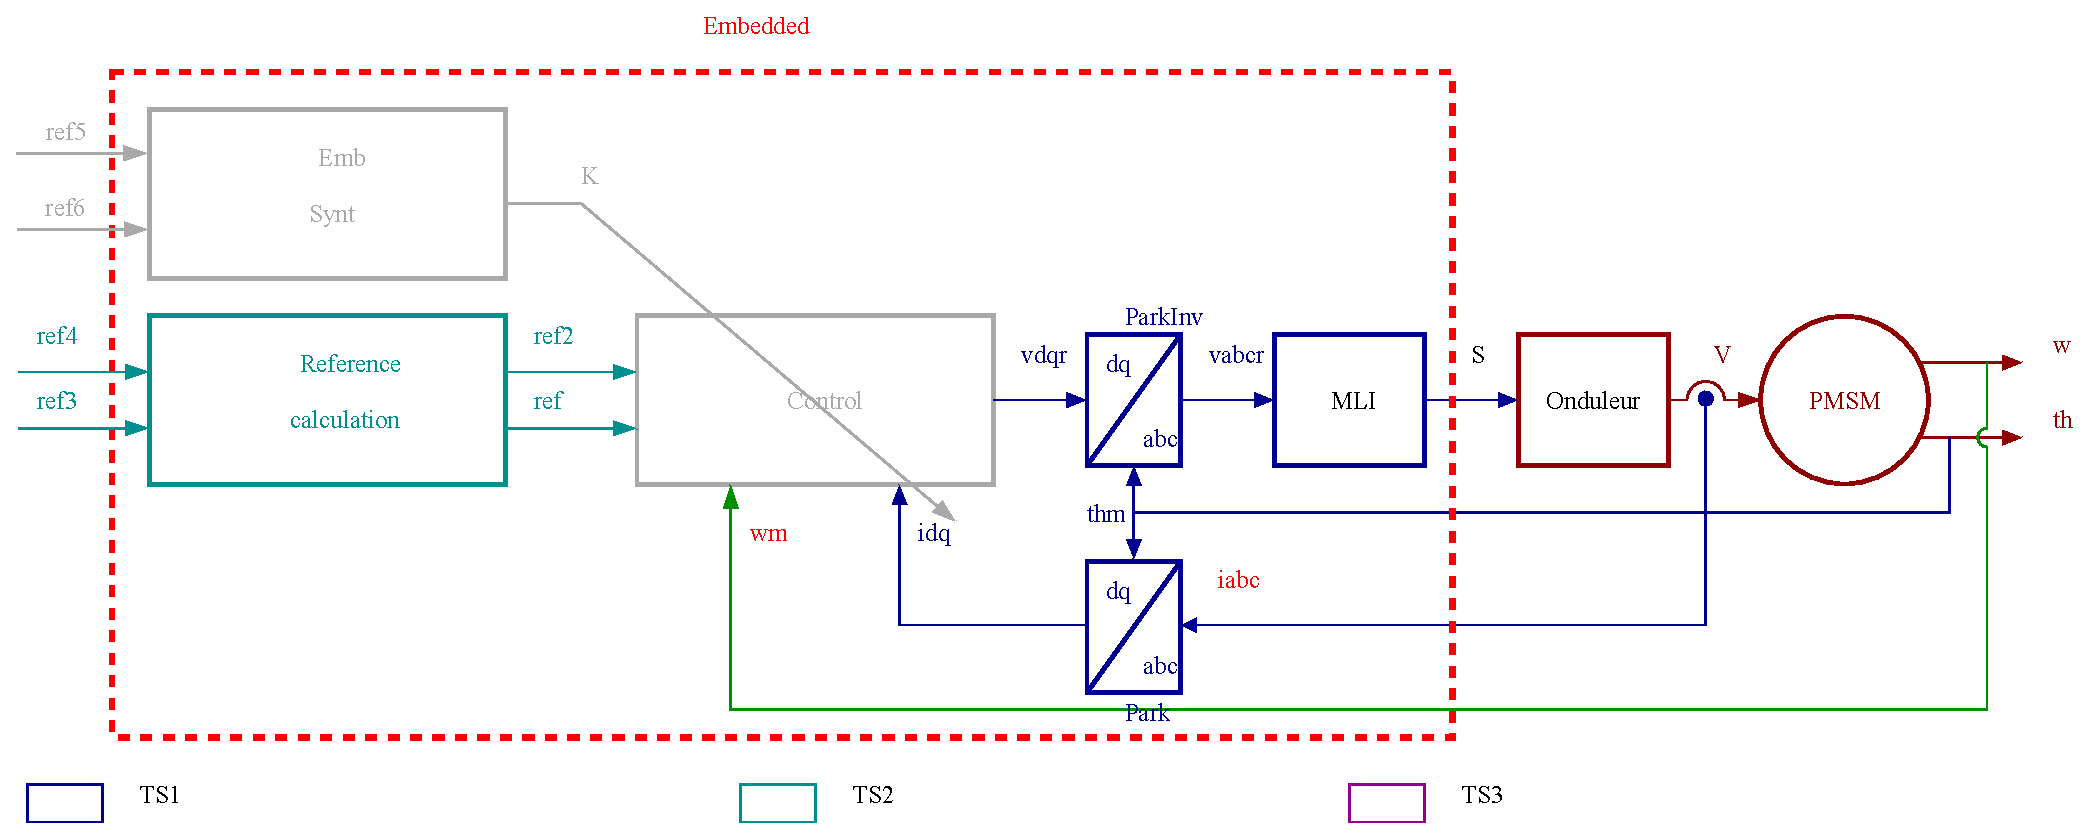
\includegraphics[width = .9\textwidth]{pictures/AdvancedControl_trajec.eps}
            \end{center}
        \label{fig:AdvancedControlForElectricalMotorTrajec}
        \end{figure}
\end{frame}


% ========================================
% Section 1: Optimal Torque Control
% ========================================
\section{Optimal torque control}


\begin{frame}{Optimal torque control}{System constraint}
    \begin{columns}
    \begin{column}{0.4\framewidth}
        \only<2>{\colorbox{lightblue}{ Objective: \textcolor{red}{Minimize Joule losses} }}
         \begin{eqnarray*}
            \only<3-4>{&\underset{i_d,i_q}{\textbf{min}} \quad i_{dq}^\top i_{dq},\quad \textbf{such that}\\}
            &\tikz[remember picture,baseline=(idqeq.base)]{\node[inner sep=0pt](idqeq){$i_{dq}^\top i_{dq} - i_{max}^2 \leqslant 0$};}\\
            %\only<1-2>{&  \tikz[remember picture,baseline=(vdqeq.base)]{\node[inner sep=0pt](vdqeq){$v_{dq}^\top v_{dq} - v_{max}^2\leqslant 0$,};} \\}
            \only<1-3>{&  \tikz[remember picture,baseline=(vdqeq.base)]{\node[inner sep=0pt,align=center](vdqeq){$\textcolor{orange}{A(\omega)} i_d^2 + \textcolor{orange}{B(\omega)}i_di_q + \textcolor{orange}{C(\omega)}i_q^2+$ \\ $ \textcolor{orange}{D(\omega)}i_d + \textcolor{orange}{E(\omega)}i_q + \textcolor{orange}{F(\omega)} \leqslant 0$};} \\}
            \only<4>{&  \tikz[remember picture,baseline=(vdqeq.base)]{\node[inner sep=0pt,align=center](vdqeq){$\textcolor{black}{A(\omega)} i_d^2 + \textcolor{black}{B(\omega)}i_di_q + \textcolor{black}{C(\omega)}i_q^2+$ \\ $ \textcolor{black}{D(\omega)}i_d + \textcolor{black}{E(\omega)}i_q + \textcolor{black}{F(\omega)} \leqslant 0$};} \\}
            %
            \only<1-3>{& \tikz[remember picture,baseline=(taueq.base)]{\node[inner sep=0pt](taueq){$\tau_{em} - \frac{3}{2}p \big( \phi_f +  (L_d - L_q) i_d \big) i_q= 0.$}; }}
            \only<4>{& \tikz[remember picture,baseline=(taueq.base)]{\node[inner sep=0pt](taueq){$\textcolor{red}{\tau_{em}} - \frac{3}{2}p \big( \phi_f +  (L_d - L_q) i_d \big) i_q= 0.$}; }}
         \end{eqnarray*}
         \tikz[remember picture,overlay] {
            %\only<1>{\draw[dashed,very thick,rounded corners,blue] ([xshift=-0.1cm,yshift=0.2cm]idqeq.north west) rectangle ([xshift=0.1cm,yshift=-0.08cm]idqeq.south east);}
            %\only<2>{\draw[dashed,very thick,rounded corners,red] ([xshift=-0.1cm,yshift=0.1cm]vdqeq.north west) rectangle ([xshift=0.1cm,yshift=-0.08cm]vdqeq.south east);}
            %\only<3>{\draw[dashed,very thick,rounded corners,red] ([xshift=-0.1cm,yshift=0.1cm]vdqeq.north west) rectangle ([xshift=0.1cm,yshift=-0.08cm]vdqeq.south east);}
            \only<4>{\draw[dashed,very thick,rounded corners,red] ([xshift=-0.1cm,yshift=0.1cm]taueq.north west) rectangle ([xshift=0.1cm,yshift=-0.08cm]taueq.south east);}
            % \node[right] at ([xshift=0.2cm]idqeq.east) {\textcolor{blue}{Electrical dynamic}};
            }
    \end{column}
    \begin{column}{0.6\framewidth}
    \centering
     %\only<1>{Current constraint in the $i_{dq}$ frame
    %     \centering
    %     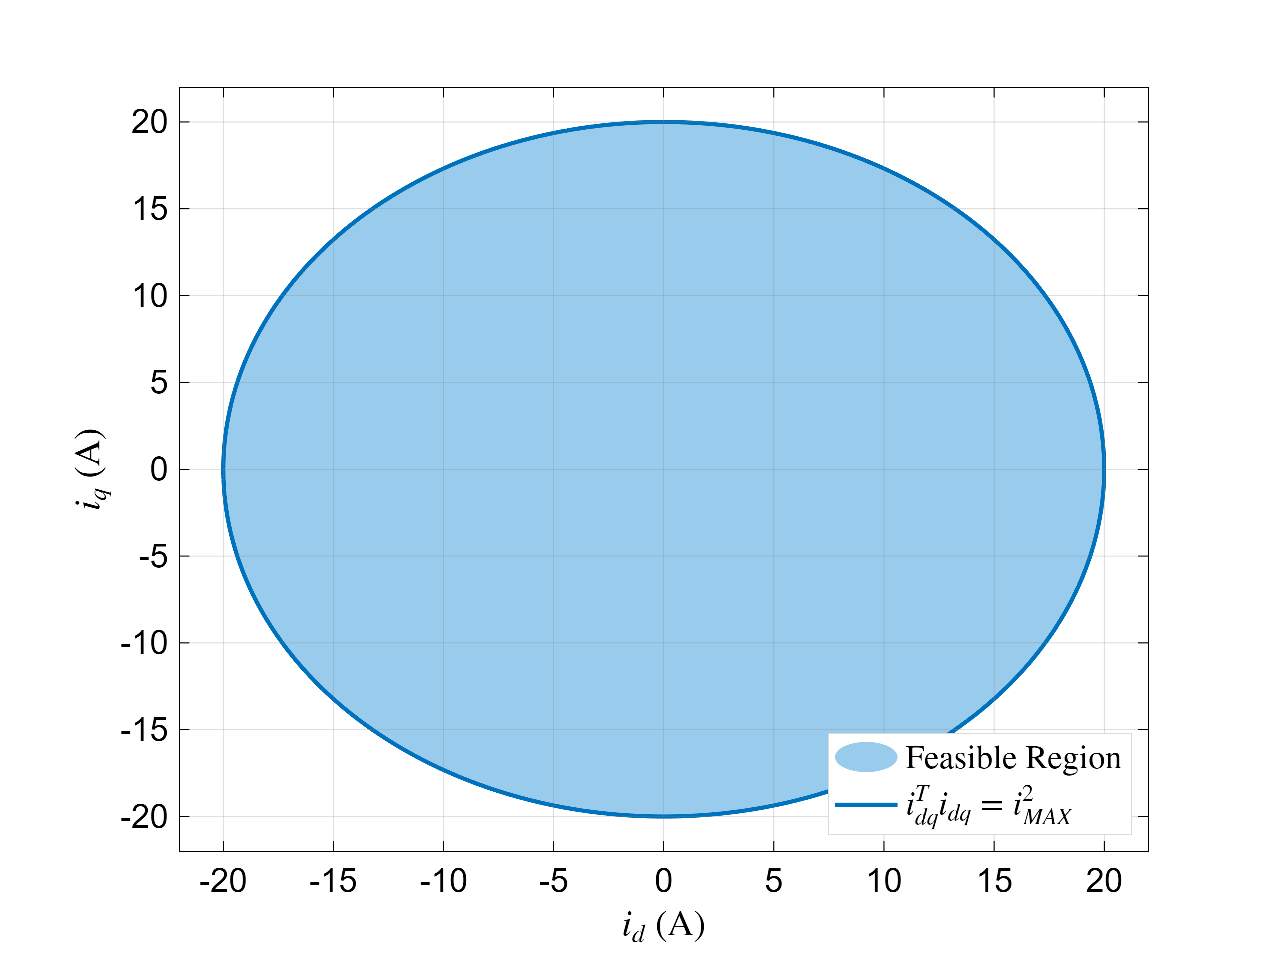
\includegraphics[width=7cm]{pictures/current_constraint_cost.eps}
    %  }
    % %  \only<2>{
    %     Voltage  constraint in the $i_{dq}$ frame
    %      \begin{eqnarray*}
    %         \cancel{L_d \frac{di_d}{dt}} &=& v_d - Ri_d +p L_q\omega i_q = 0, \\
    %         \cancel{L_q\frac{di_q}{dt}} &=& v_q -Ri_q -pL_d\omega i_d -p \phi_f\omega = 0,
    %    \end{eqnarray*}
    %  }
    %  \only<3>{
    %  \begin{center}
    %       \animategraphics[loop,controls,width=1\textwidth]{10}{eps_frames_voltage_animation_filled_with_cost/frame_}{000}{040}
    %   \end{center}
    %  }
     \only<1-2>{
      \begin{center}
         % \animategraphics[loop,controls,width=1\textwidth]{10}{eps_frames_voltage_cost_torque/frame_}{000}{040}
         %%%%%%%%%%%%%%%%%%%%Here Here here 
         \animategraphics[loop,controls,width=1\textwidth]{10}{eps_frames_voltage_animation_torque/frame_}{000}{040}
      \end{center}
     }
     \only<3>{\animategraphics[loop,controls,width=1\textwidth]{10}{eps_frames_voltage_cost_torque_optimal/frame_}{000}{040}
     }
     \only<4> {\animategraphics[loop,controls,width=1\textwidth]{10}{eps_frames_torque_cost_speed_optimal/frame_}{000}{014}
     }
    \end{column}
    \end{columns}
\end{frame}



\subsection{Literature}
\begin{frame}{Optimal torque control}{Literature}
\begin{columns}
    \begin{column}{0.5\framewidth}
    The classical optimal torque control problem:
    \vspace{+0.3cm}
        \begin{eqnarray*}
            &\underset{i_d,i_q}{\textbf{min}} \quad i_{dq}^\top i_{dq},\quad \textbf{such that}\\
            & i_{dq}^\top i_{dq} - i_{max}^2 \leqslant 0\\
            & A(\omega) i_d^2 + B(\omega)i_di_q + C(\omega)i_q^2+ \\
            & \quad D(\omega)i_d + E(\omega)i_q + F(\omega) \leqslant 0\\
            & \tikz[remember picture,baseline=(taueq.base)]{\node[inner sep=0pt](taueq){$ \tau_{em} - \frac{3}{2}p \big( \phi_f +  (L_d - L_q) i_d \big) i_q= 0.$}}
        \end{eqnarray*}
        \tikz[remember picture,overlay] {
        \draw[dashed,very thick,rounded corners,red] ([xshift=-0.1cm,yshift=0.1cm]taueq.north west) rectangle ([xshift=0.1cm,yshift=-0.08cm]taueq.south east);}
    \end{column}
    \begin{column}{0.5\framewidth}
        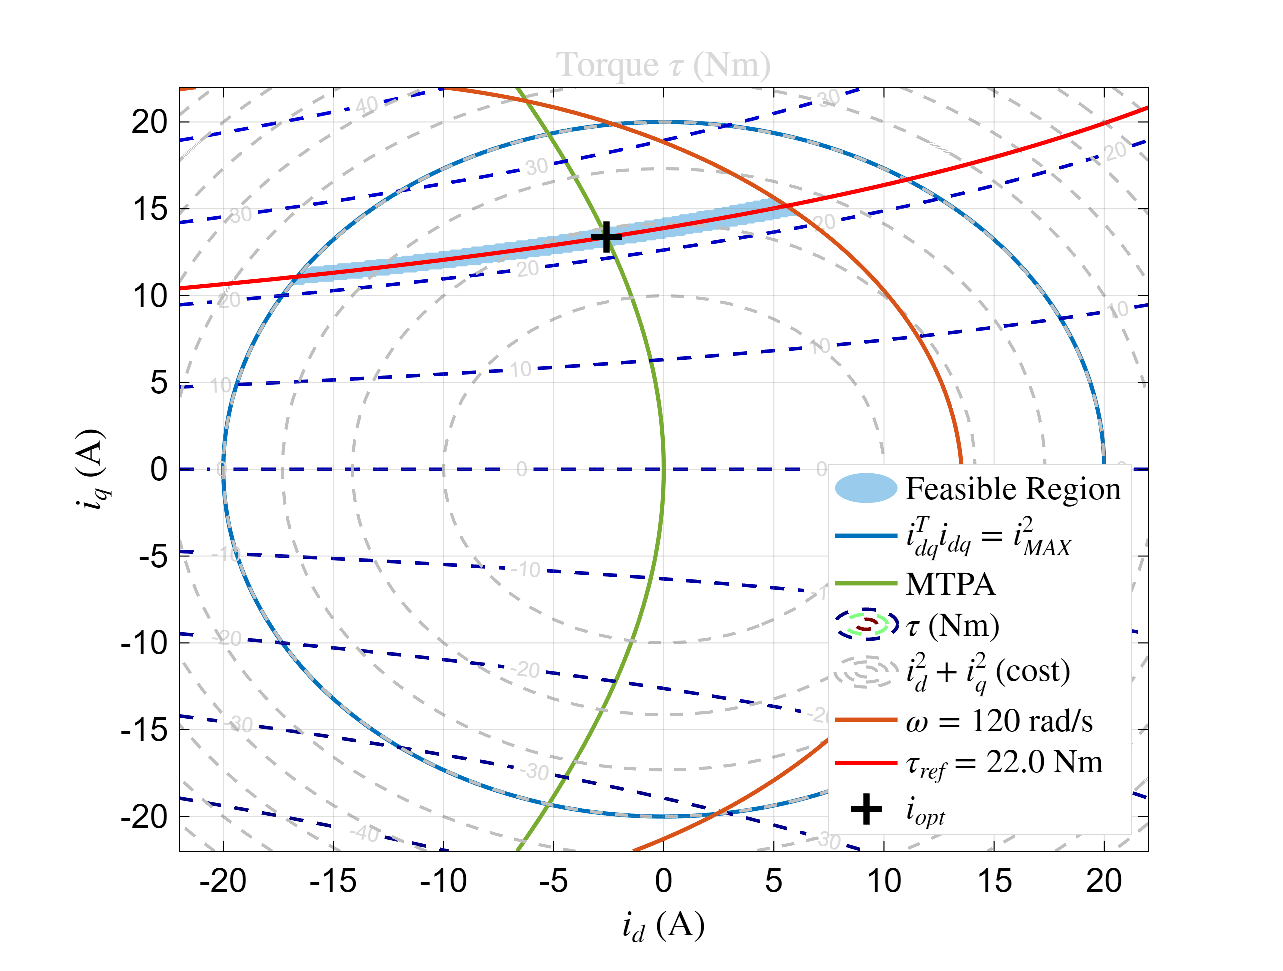
\includegraphics[width=1\columnwidth]{eps_frames_torque_cost_speed_optimal/frame_010}
        %eps_frames_voltage_animation_torque/frame_
    \end{column}
\end{columns}
\textbf{Challenge:} the torque constraint is \textcolor{red}{nonconvex}
\end{frame}

\begin{frame}{Optimal torque control}{Classical approach: Decision tree \footnote{H. Eldeeb et al., "\textbf{A unified theory for optimal feedforward torque control of anisotropic synchronous machines}," \textit{International Journal of Control}, pp. 2273–2302, Oct. 2018.}}
    \begin{columns}[T] % [T] aligns the tops of the columns
        \begin{column}{0.4\textwidth}
            \textbf{Literature approach:} \textcolor{Blue}{\textbf{Decision tree}}

            \vspace{0.4cm}
            \textbf{Operating zones:}
            \begin{itemize}
                \item \textcolor{blue}{MTPC}: No constraint active
                \item \textcolor{orange}{Maximum Current}: Current constraint active
                \item \textcolor{green!60!black}{Field Weakening}: Voltage constraint active
                \item \textcolor{cyan!60!black}{MTPV}: Both constraints active
            \end{itemize}
        \end{column}

        \begin{column}{0.5\textwidth}
            \only<1->{
                \vspace{-1cm}
                    \begin{figure}
                    \centering
                    \includegraphics[width=1.1\columnwidth]{pictures/decision_tree_hq.eps}
                    \caption{Optimal torque control decision tree}
                    \end{figure}
            }
        \end{column}
    \end{columns}
    \only<2>{
     \vspace{0.1cm}
    \begin{center}
    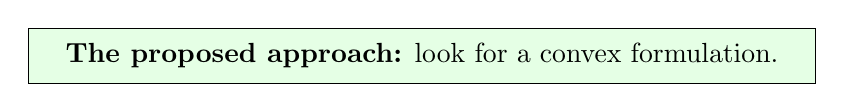
\begin{tikzpicture}
        \node[draw, rectangle, fill=green!10, minimum width=10cm, minimum height=0.7cm] {
            \begin{minipage}{9.5cm}
                \centering
                \textbf{The proposed approach:} look for a convex formulation. 
            \end{minipage}
        };
    \end{tikzpicture}
    \end{center}
    }
\end{frame}


\begin{frame}{Optimal torque problem}{Advantages of the proposed convex formulation \footnote{S. Boyd and L. Vandenberghe, "\textbf{Convex Optimization}," Cambridge University Press, 2004.}}

    \vspace{0.2cm}
    \begin{columns}[t]
        \begin{column}{0.48\framewidth}
            \textbf{The \textcolor{Blue}{convex} formulation}
            \begin{itemize}

                \item \textcolor{Blue}{\textbf{Solvers with polynomial complexity}}
                \item \textcolor{Blue}{\textbf{Scales efficiently}} to complex scenarios
                \item \textcolor{Blue}{\textbf{Easy to add constraints}}
                \item \textcolor{Blue}{\textbf{Guaranteed convergence}} to global optimum
                \item \textcolor{Blue}{\textbf{Easy to integrate}}
                \item \textcolor{Blue}{\textbf{Unified solution}} 
            \end{itemize}
        \end{column}
    %\end{columns}

            \begin{column}{0.48\framewidth}
            \textbf{Decision tree approach:}
            \begin{itemize}
                \item Combinatorial complexity when adding constraints
                \item Difficult to scale up the problem
                 \item Case-by-case analysis for each operating region
            \end{itemize}
        \end{column}
   % \vspace{0.4cm}
    \end{columns}

%     \vspace{0.3cm}
%     \begin{center}
%     \begin{tikzpicture}
%         \node[draw, rectangle, fill=green!10, minimum width=10cm, minimum height=0.7cm] {
%             \begin{minipage}{9.5cm}
%                 \centering
%                 \textbf{Example:} Control $N$ PMSMs on the same power source 
%             \end{minipage}
%         };
%     \end{tikzpicture}
%     \end{center}
 \end{frame}

% \begin{frame}{Optimal torque control}{The proposed approach}
%     \begin{columns}[T] % optional: align top
%         % Left column
%         \begin{column}{0.5\textwidth}
%             \begin{eqnarray*}
%                 &\underset{i_d,i_q}{\textbf{min}} \quad i_d^2+i_q^2,\quad \textbf{such that}\\
%                 & i_{dq}^\top i_{dq} - i_{max}^2 \leqslant 0\\
%                 & A(\omega) i_d^2 + B(\omega)i_di_q + C(\omega)i_q^2+ \\
%                 & \quad D(\omega)i_d + E(\omega)i_q + F(\omega) \leqslant 0\\
%                 & \tikz[remember picture,baseline=(taueq.base)]{\node[inner sep=0pt](taueq){$ \tau - \frac{3}{2}p \big( \phi_f +  (L_d - L_q) i_d \big) i_q= 0.$}}
%             \end{eqnarray*}

%             \begin{center}
%                 \begin{tikzpicture}
%                     \node[draw, rectangle, fill=red!10, minimum width=7cm, minimum height=0.8cm] {
%                         \begin{minipage}{6.5cm}
%                             \centering
%                             \textbf{How to make the problem convex ?}
%                         \end{minipage}
%                     };
%                 \end{tikzpicture}
%             \end{center}

%             \pause
%         \end{column}

%         % Right column
%         \begin{column}{0.5\textwidth}
%             \textbf{The proposed solution:}
%             \begin{center}
%                 \begin{tikzpicture}
%                     \node[draw, rectangle, fill=green!10, minimum width=7cm, minimum height=0.8cm] {
%                         \begin{minipage}{6.5cm}
%                             \centering
%                             \textbf{A change of variable}
%                         \end{minipage}
%                     };
%                 \end{tikzpicture}

%                 \begin{equation*}
%                     i_q = \frac{2}{3p} \frac{\tau}{\phi_f+(L_d-L_q)i_d}.
%                 \end{equation*}
%             \end{center}
%         \end{column}
%     \end{columns}
% \end{frame}

\begin{frame}{Optimal torque control}{The proposed approach}
\begin{columns}[T]

% Left column
\begin{column}{0.5\textwidth}
    \only<1->{
    \textbf{The classical problem:}
\begin{eqnarray*}
&\underset{i_d,i_q}{\textbf{min}} \quad i_{dq}^\top i_{dq},\quad \textbf{such that}\\
& i_{dq}^\top i_{dq} - i_{max}^2 \leqslant 0\\
& A(\omega) i_d^2 + B(\omega)i_di_q + C(\omega)i_q^2+ \\
& \quad D(\omega)i_d + E(\omega)i_q + F(\omega) \leqslant 0\\
& \tikz[remember picture,baseline=(taueq.base)]{\node[inner sep=0pt](taueq){$ \tau_{em} - \frac{3}{2}p \big( \phi_f +  (L_d - L_q) i_d \big) i_q= 0.$}}
\end{eqnarray*}

\begin{center}
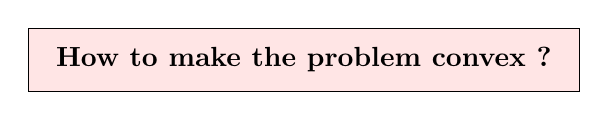
\begin{tikzpicture}
\node[draw,rectangle,fill=red!10,minimum width=7cm,minimum height=0.8cm]{
\begin{minipage}{6.5cm}\centering\textbf{How to make the problem convex ?}\end{minipage}};
\end{tikzpicture}
\end{center}
    }


\end{column}

% Right column
\begin{column}{0.5\textwidth}
    \only<2->{
\textbf{The proposed reformulation:}
\begin{center}
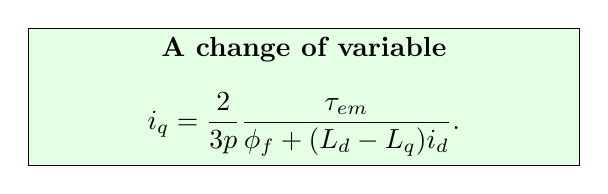
\begin{tikzpicture}
\node[draw,rectangle,fill=green!10,minimum width=7cm,minimum height=0.8cm]{
\begin{minipage}{6.5cm}\begin{center}

\textbf{A change of variable}
\begin{equation*} i_q=\frac{2}{3p}\frac{\tau_{em}}{\phi_f+(L_d-L_q)i_d}. \end{equation*} \end{center}
\end{minipage}};
\end{tikzpicture}
\end{center}
    }
    \only<3->{
The new problem is
\begin{center}
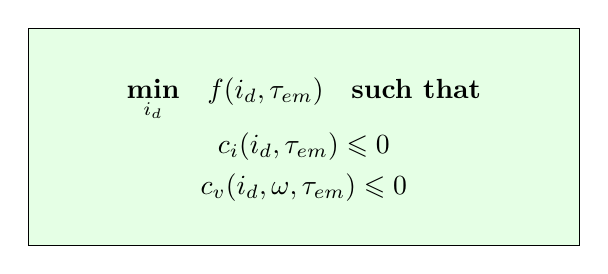
\begin{tikzpicture}
\node[draw,rectangle,fill=green!10,minimum width=7cm,minimum height=0.8cm]{
\begin{minipage}{6.5cm}
    \begin{center}
\begin{eqnarray*}
&\underset{i_d}{\textbf{min}} \quad f(i_d,\tau_{em})\quad \textbf{such that}\\
&c_i(i_d,\tau_{em})\leqslant0\\
&c_v(i_d,\omega,\tau_{em})\leqslant0\\
\end{eqnarray*}
 \end{center}
\end{minipage}};

\end{tikzpicture}
\end{center}
    }

\end{column}
\end{columns}
    \only<4>{\textbf{\textcolor{Blue}{Is the problem convex?}}
    over the set $\mathcal{S} =  \{(i_d, \omega, \tau_{em}) \in \mathbb{R}^3 \:|\: -i_{max} \leqslant i_d \leqslant 0, \: \omega \geqslant 0, \: \tau_{em} \geqslant 0\} $
    }

\end{frame}

\begin{frame}{Optimal torque control problem}{Convexity of the proposed formulation}
\textbf{Question:} Is the reformulated problem convex over $\mathcal{S}$?
\begin{equation*}
\underset{i_d}{\textbf{min}} \quad f(i_d,\tau_{em})\quad \textbf{s.t.}\quad
c_i(i_d,\tau_{em})\leqslant0, \quad c_v(i_d,\omega,\tau_{em})\leqslant0
\end{equation*}

% \only<1>{
% \vspace{0.2cm}
% \begin{block}{Convexity requirements}
% \begin{itemize}
%     \item Objective $f$: \textcolor{blue}{\textbf{convex}} ($f'' \geq 0$)
%     \item Constraints $g_i(x) \leq 0$: \textcolor{blue}{\textbf{convex}} functions
% \end{itemize}
% \end{block}
% }

%\only<2>{
    \vspace{0.3cm}
    \textbf{Analysis over $\mathcal{S}$:}
    \begin{itemize}
        \item[$\checkmark$]  $f(i_d,\tau_{em})$ is \textcolor{blue}{\textbf{convex}}
        \item[$\checkmark$]  $c_i(i_d,\tau_{em})\leqslant 0$ is \textcolor{blue}{\textbf{convex}}
        \item[$\boldsymbol{?}$]  $c_v(i_d,\omega,\tau_{em})\leqslant 0$ is \textcolor{red}{\textbf{convex}} ?
    \end{itemize}
    \vspace{0.3cm}
    \begin{center}
    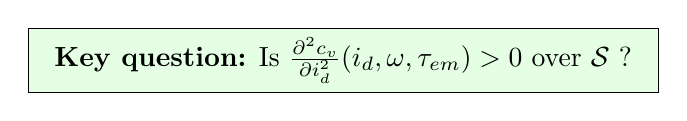
\begin{tikzpicture}
    \node[draw,rectangle,fill=green!10,minimum width=8cm,minimum height=0.8cm]{
    \begin{minipage}{7.5cm}\centering
    \textbf{Key question:} Is $\frac{\partial^2 c_v}{\partial i_d^2}(i_d, \omega, \tau_{em} ) > 0$ over $\mathcal{S}$ ?
    \end{minipage}};
    \end{tikzpicture}
    \end{center}
%}
\end{frame}


\begin{frame}{Optimal torque control problem}{Convexity analysis: Voltage constraint}
    \vspace{-0.2cm}
    \textbf{Key question:} Is $\frac{\partial^2 c_v}{\partial i_d^2}(i_d, \omega, \tau_{em} ) > 0$ over $\mathcal{S}$ ?

    %\pause
    \vspace{0.2cm}
    \textbf{Approach:} Multiply by a positive term to simplify
    \begin{equation*}
        h(i_d, \omega, \tau_{em}) = \underbrace{(K_1+K_2 i_d)^4}_{>0} \cdot \frac{\partial^2 c_v}{\partial i_d^2}(i_d, \omega, \tau_{em} )
    \end{equation*}

    \pause
    \vspace{0.1cm}
    This gives a polynomial:
    \begin{equation*}
        h(i_d, \omega, \tau_{em}) = a_4 i_d^4 + a_3 i_d^3 + a_2 i_d^2 + a_1 i_d + a_0
    \end{equation*}
    where $a_i = a_i(\omega,\tau_{em})$

    \pause
    \vspace{0.2cm}
    \begin{center}
    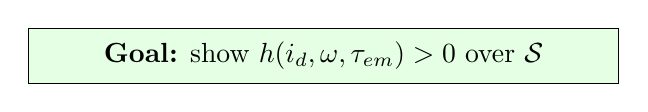
\begin{tikzpicture}
    \node[draw,rectangle,fill=green!10,minimum width=7.5cm,minimum height=0.7cm]{
    \begin{minipage}{7cm}\centering
    \textbf{Goal:} show $h(i_d,\omega,\tau_{em}) > 0$ over $\mathcal{S}$
    \end{minipage}};
    \end{tikzpicture}
    \end{center}
\end{frame}

\begin{frame}{Optimal torque control problem}{Sum-of-Squares (SOS) decomposition}
    \vspace{-0.2cm}
    \textbf{Recall the goal:}
    \begin{center}
    \vspace{-0.1cm}
    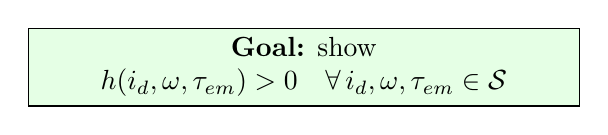
\begin{tikzpicture}
    \node[draw,rectangle,fill=green!10,minimum width=7cm,minimum height=0.7cm]{
    \begin{minipage}{5.5cm}\centering
    \textbf{Goal:} show $h(i_d,\omega,\tau_{em})> 0 \quad \forall \, i_d, \omega, \tau_{em} \in \mathcal{S}$
    \end{minipage}};
    \end{tikzpicture}
    \vspace{-0.1cm}
    \end{center}

    \pause
    \textbf{Proposed approach:} Show that $h$ admits a \textcolor{blue}{\textbf{SoS decomposition}} over $\mathcal{S}$:
    \vspace{-0.1cm}
    \begin{equation*}
        h(i_d,\omega,\tau_{em}) = \textcolor{blue}{s_0} + \textcolor{blue}{s_1}\underbrace{(i_d+i_{max})}_{\geq 0} + \textcolor{blue}{s_2}\underbrace{(-i_d)}_{\geq 0} + \textcolor{blue}{s_3}\underbrace{\omega}_{\geq 0} + \textcolor{blue}{s_4}\underbrace{\tau_{em}}_{\geq 0} \quad \textcolor{blue}{\textbf{(Positivstellensatz)}}
    \end{equation*} 
    \vspace{-0.1cm}
    where each $\textcolor{blue}{s_j}$ is a \textcolor{blue}{\textbf{SoS polynomial}}

    \pause
    \vspace{0.1cm}
    \textbf{What is Sum-of-Squares (SOS)?}
    \vspace{0.1cm}
    \begin{itemize}
        \setlength{\itemsep}{2pt}
        \item Each $\textcolor{blue}{s_j}$ is a \textcolor{blue}{\textbf{sum of squares}}: $s_j = \sum_{k} p_{j,k}^2 \geqslant 0$. \textit{Ex:} $s_0 = (i_d + \omega)^2 + (2\tau_{em} - 1)^2$
        \pause
        %\item Over $\mathcal{S}$, multipliers $(i_d+i_{max})$, $(-i_d)$, $\omega$, $\tau$ are $\geq 0$
        %\pause
        %\item Thus: $h = s_0 + s_1 (i_d+i_{max}) + \cdots \geq 0$ over $\mathcal{S}$ \textcolor{blue}{\textbf{(Positivstellensatz)}}
       % \pause
        \item SOS found via \textcolor{blue}{\textbf{semidefinite programming}} (YALMIP + MOSEK)
    \end{itemize}
\end{frame}

\begin{frame}{Optimal torque control problem}{Convexity via hybrid analytical-SoS approach}
    \begin{proposition}
    For a given PMSM, the reformulated problem is \textcolor{blue}{\textbf{convex}} if one of the following holds:

    \vspace{0.2cm}
    \textcolor{red}{\textbf{1.}} \textbf{Direct SoS approach:} $h$ admits a SoS decomposition
    \begin{equation*}
        h(i_d,\omega,\tau_{em}) = s_0 + s_1(i_d+i_{max}) + s_2(-i_d) + s_3\omega + s_4\tau_{em}
    \end{equation*}
    where each $s_j$ is a \textcolor{blue}{\textbf{SoS polynomial}}.

    \only<1>{
    \vspace{0.2cm}
    \textcolor{gray}{\textcolor{red}{\textbf{2.}} \textbf{Hybrid approach:} $h = h_1 + h_2$ with}
    \begin{equation*}
        \textcolor{gray}{
        \begin{cases}
            h_1(i_d,\omega,\tau_{em}) \geqslant 0 \text{ (proven analytically), } \quad \forall (i_d,\omega, \tau_{em}) \in \mathcal{S}\\
            h_2(i_d,\omega,\tau_{em}) = s_0 + s_1(i_d+i_{max}) + s_2(-i_d) + s_3\omega + s_4\tau_{em}
        \end{cases}
        }
    \end{equation*}
    \textcolor{gray}{where each $s_j$ is a SoS polynomial, ensuring $h \geqslant 0$ over $\mathcal{S}$.}
    }

    \only<2>{
    \vspace{0.2cm}
    \textcolor{red}{\textbf{2.}} \textbf{Hybrid approach:} $h = h_1 + h_2$ with
    \begin{equation*}
        \begin{cases}
            h_1(i_d,\omega,\tau_{em}) \geqslant 0 \text{ (\textcolor{blue}{\textbf{proven analytically}}), } \quad \forall (i_d,\omega, \tau_{em}) \in \mathcal{S}\\
            h_2(i_d,\omega,\tau_{em}) = s_0 + s_1(i_d+i_{max}) + s_2(-i_d) + s_3\omega + s_4\tau_{em}
        \end{cases}
    \end{equation*}
    where each $s_j$ is a \textcolor{blue}{\textbf{SoS polynomial}}, ensuring $h \geqslant 0$ over $\mathcal{S}$.
    }

    \vspace{0.2cm}
    {\small where $h(i_d, \omega, \tau_{em}) = (K_1+K_2 i_d)^4 \cdot c_v''(i_d, \omega, \tau_{em})$ and $\mathcal{S} = \{(i_d, \omega, \tau_{em}) \in \mathbb{R}^3 \:|\: -i_{max} \leqslant i_d \leqslant 0, \: \omega \geqslant 0, \: \tau_{em} \geqslant 0\}$.}
    \end{proposition}
\end{frame}

% \subsection{Direct SoS approach}
% \begin{frame}{Optimal torque control problem}{Proof sketch: Direct SoS approach}
%     %\begin{proof}
%     If $h$ admits the SoS decomposition
%     \begin{equation*}
%         h(i_d,\omega,\tau) = s_0 + s_1(i_d+i_{max}) + s_2(-i_d) + s_3\omega + s_4\tau
%     \end{equation*}
%     where each $s_j$ is a \textcolor{green}{\textbf{SoS polynomial}}, then:

%     \pause
%     \vspace{0.2cm}
%     \textbf{Step 1:} Each $s_j$ is a sum of squares, so
%     \begin{equation*}
%         s_j(i_d,\omega,\tau) = \sum_{k} p_{j,k}^2(i_d,\omega,\tau) \geqslant 0, \quad \forall (i_d,\omega,\tau) \in \mathbb{R}^3
%     \end{equation*}
%     \textit{Example:} $s_0(i_d,\omega,\tau) = (i_d + \omega)^2 + (2\tau - 1)^2 + \omega^2$ is a SoS polynomial

%     \pause
%     \vspace{0.2cm}
%     \textbf{Step 2:} Over the domain $\mathcal{S} = \{(i_d, \omega, \tau) \in \mathbb{R}^3 \:|\: -i_{max} \leqslant i_d \leqslant 0, \: \omega \geqslant 0, \: \tau \geqslant 0\}$, the multipliers are non-negative:
%     \begin{equation*}
%         \underbrace{(i_d+i_{max})}_{\geqslant 0}, \quad \underbrace{(-i_d)}_{\geqslant 0}, \quad \underbrace{\omega}_{\geqslant 0}, \quad \underbrace{\tau}_{\geqslant 0}
%     \end{equation*}

%     \pause
%     \vspace{0.2cm}
%     \textbf{Step 3:} Therefore, $h(i_d,\omega,\tau) \geqslant 0$ over $\mathcal{S}$ (\textcolor{blue}{\textbf{Positivstellensatz certificate}}).

%     \pause
%     \vspace{0.2cm}
%     This certificate can be \textcolor{green}{\textbf{found computationally}} using semidefinite programming (YALMIP + MOSEK).
%    % \end{proof}
% \end{frame}

% \begin{frame}{Optimal torque control problem}{Drawbacks of direct SOS approach}
%         \textbf{Challenge:} Direct SoS decomposition of the entire polynomial may be:
%     \begin{itemize}
%         \item Computationally expensive (high degree, many variables)
%         \item Numerically difficult to find
%         \item May not exist for a fixed degree of polynomial $s_j$ even when $h \geqslant 0$ is true
%     \end{itemize}
% \end{frame}
% \subsection{Proof sketch}
% \begin{frame}{Optimal torque control problem}{Proof sketch: Hybrid analytical-SOS approach}
%     \textbf{Goal:} Prove that a polynomial $h(i_d, \omega, \tau) \geqslant 0$ over domain $\mathcal{S}$.

%     \pause
%     \vspace{0.3cm}
%     \textcolor{blue}{\textbf{Key idea:}} Decompose $h = h_1 + h_2$ where:
%     \begin{center}
%     \begin{tabular}{cc}
%         \tikz[baseline]{\node[rectangle, draw=green!60!black, thick, fill=green!10, inner sep=5pt, align=center] (analytical) {
%             \textbf{Analytical proof} \\[0.2cm]
%             Part of polynomial \\
%             where signs are \\
%             easy to determine
%         };}
%         &
%         \tikz[baseline]{\node[rectangle, draw=orange!60!black, thick, fill=red!10, inner sep=5pt, align=center] (sos) {
%             \textbf{SoS proof} \\[0.2cm]
%             Remaining part \\
%             where SoS \\
%             is more tractable
%         };}
%     \end{tabular}

%     \end{center}

% \end{frame}

\subsection{Practical example}
\begin{frame}{Optimal torque control problem}{A practical example PMSM}
    \vspace{-0.3cm}
    Consider the PMSM test bench available in the Ampère Laboratory:
\begin{columns}
    \begin{column}{0.5\framewidth}
        \begin{table}[!h]
            \small
            %\caption{PMSM parameters.}
            \centering
            \begin{tabular}{cc}
            \toprule
            \textbf{Parameter} & \textbf{PMSM}\\
                \midrule
                Resistance $R$ $(\Omega)$        & 0.9\\
                $d$-axis inductance $L_d$ $(mH)$   & 0.012\\
                $q$-axis inductance $L_q$ $(mH)$   & 0.020\\
                Flux constant $\phi_f$ $(mWb)$  	 & 0.264\\
                Pole pairs $p$       			 & 4     \\
                DC voltage $v_{\mathrm{DC}}$ $(V)$ & 600 \\
                Maximum power $P$ $(kW)$		     & 15\\
                \bottomrule
            \end{tabular}
            \label{tab:IPMSM_parameters}
        \end{table}
    \end{column}
    \begin{column}{0.5\framewidth}
        \begin{figure}[H]
            \centering
            \includegraphics[trim={0cm 5cm 2cm 0cm},clip,width=0.8\textwidth]{pictures/Banc_IPMSM.eps}
            \caption{ PMSM test bench.}
            \label{fig:bancIPMSM}
        \end{figure}
    \end{column}
\end{columns}
    \begin{equation*}
        h(i_d, \omega, \tau_{em}) = \tikz[remember picture,baseline=(h1.base)]{\node[inner sep=2pt](h1){$\textcolor{blue}{\underbrace{a_4(\omega,\tau_{em}) i_d^4 + a_3(\omega,\tau_{em}) i_d^3 + a_2(\omega,\tau_{em}) i_d^2}_{h_1(i_d,\omega, \tau_{em})}}$};} + \tikz[remember picture,baseline=(h2.base)]{\node[inner sep=2pt](h2){$\textcolor{red}{\underbrace{a_1(\omega,\tau_{em}) i_d + a_0(\omega,\tau_{em})}_{h_2(i_d, \omega,\tau_{em} )}}$};}
    \end{equation*}
    \vspace{-0.1cm}
    \begin{itemize}
        \item $h_1(i_d,\omega,\tau_{em}) > 0 \quad \forall\, i_d,\,\omega,\, \tau_{em} \in \mathcal{S}$ is shown analytically
        \item $h_2(i_d,\omega,\tau_{em}) > 0 \quad \forall\, i_d,\,\omega,\, \tau_{em} \in \mathcal{S}$ is shown through SoS decomposition
    \end{itemize}
\end{frame}

\begin{frame}{Optimal torque control problem}{A practical example PMSM}
\begin{columns}
    \begin{column}{0.5\textwidth}
        The optimal torque control problem
        \begin{eqnarray*}
&\underset{i_d}{\textbf{min}} \quad f(i_d,\tau_{em})\quad \textbf{such that}\\
&c_i(i_d,\tau_{em})\leqslant0\\
&c_v(i_d,\omega,\tau_{em})\leqslant0\\
\end{eqnarray*}
over the domain of definition $\mathcal{S}$ is \textbf{\textcolor{OliveGreen}{convex}}

 \only<2>{
    \vspace{+0.5cm}
We implement:
 \begin{center}
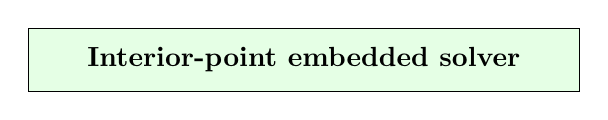
\begin{tikzpicture}
\node[draw,rectangle,fill=green!10,minimum width=7cm,minimum height=0.8cm]{
\begin{minipage}{6.5cm}\begin{center}
\textbf{Interior-point embedded solver}
\end{center}\end{minipage}};
\end{tikzpicture}
\end{center}
 }
    \end{column}
    \begin{column}{0.5\textwidth}
            \begin{figure}[H]
            \centering
            \includegraphics[trim={0cm 5cm 2cm 0cm},clip,width=0.8\textwidth]{pictures/Banc_IPMSM.eps}
            \caption{ PMSM test bench.}
            \label{fig:bancIPMSM}
        \end{figure}
    \end{column}
\end{columns}

\end{frame}
\begin{frame}{Optimal torque control problem}{Experiment results}


    \begin{columns}
        \begin{column}{0.5\textwidth}
            \begin{figure}[h!]
            \centering
                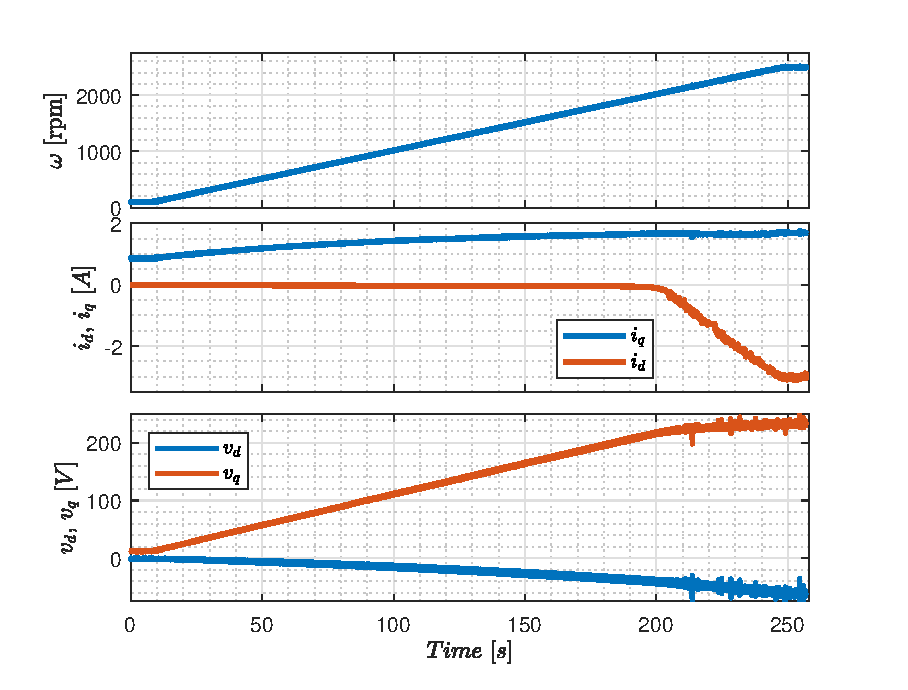
\includegraphics[width=1\columnwidth]{pictures/speed_idq_vdq1.eps}
            \end{figure}
        \end{column}
        \begin{column}{0.5\textwidth}
             \begin{figure}[h!]
            \centering
                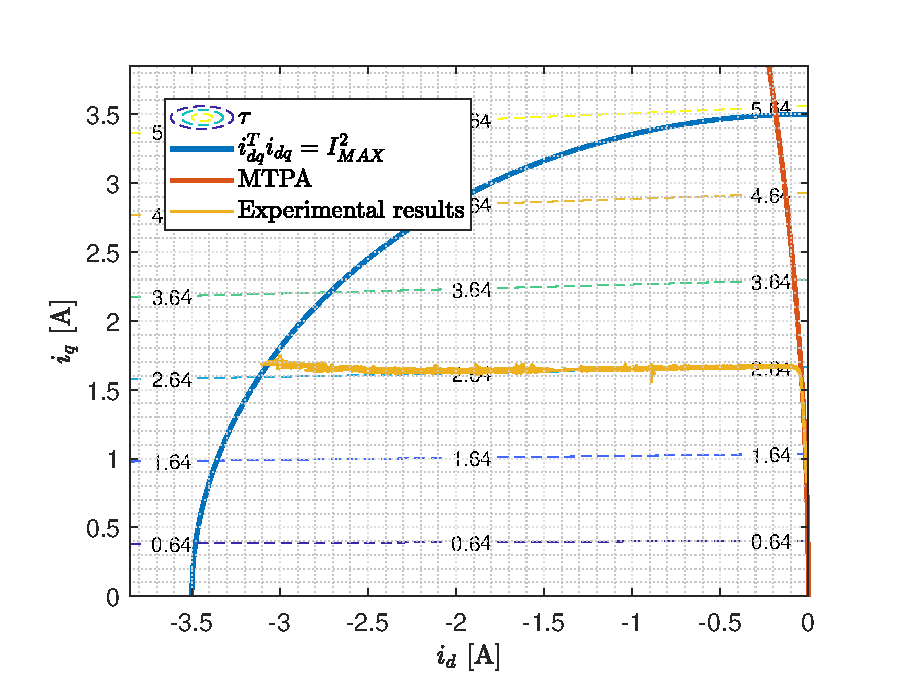
\includegraphics[width=1\columnwidth]{pictures/expe_idq_solver.eps}
            \end{figure}
        \end{column}
    \end{columns}

%     \vspace{-0.3cm} \begin{figure}[h!]
%     \centering
%     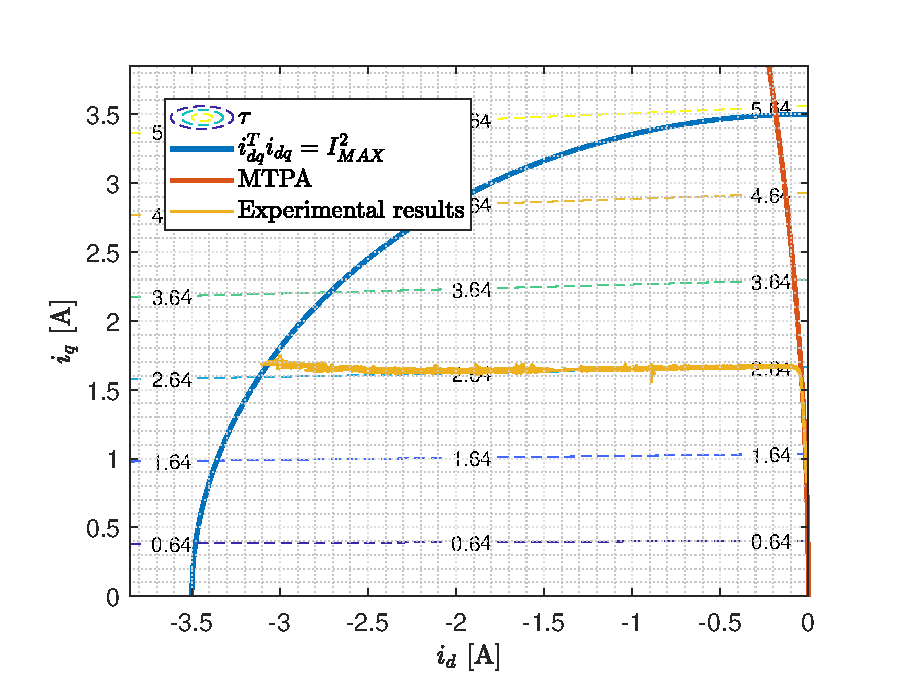
\includegraphics[width=0.7\textwidth]{pictures/expe_idq_solver.eps}
%     %\caption{Currents $i_{dq}$ trajectory in the $dq$ frame}
%     \label{fig:Experimental_Validation_Idq}
% \end{figure}
\end{frame}

\begin{frame}{Result Summary}
    \textbf{Challenge:} A nonconvex Optimal torque control problem
    \vspace{+0.2cm}
    %\textbf{Optimal Torque Control: Key achievements}

    \vspace{0.2cm}
    \begin{columns}
        \begin{column}{0.5\textwidth}
            \textbf{Theoretical contributions:}
            \begin{itemize}
                \item Change of variable
                \item New formulation of OTC problem
                \item Proof of Convexity via Sum-of-Squares programming
            \end{itemize}

            \vspace{0.1cm}
            \textbf{Implementation:}
            \begin{itemize}
                \item Interior-point embedded solver
            \end{itemize}
        \end{column}

        \begin{column}{0.5\textwidth}
            \textbf{Advantages:}
            \begin{itemize}
                \item[$+$] Polynomial complexity solvers
                \item[$+$] Scales well
                \item[$+$] Easy integration into larger convex problems
                \item[$+$] Unified solution for all operating regions
                \item[$+$] Experimental validation on PMSM test bench
            \end{itemize}
        \end{column}
    \end{columns}

    % \vspace{0.3cm}C
    % \centering
    % \textcolor{OliveGreen}{\textbf{$\Rightarrow$ Guaranteed convex optimization for optimal torque control}}
\end{frame}

\begin{frame}{Outline}
        % The outline
                \textbf{Objectives:}
    \vspace{0.2cm}
    \begin{enumerate}
        \item[\textcolor{darkgray}{\textbf{Part 1:}}] \textcolor{darkgray}{\textbf{Optimal currents $i_d^\#$, $i_q^\#$ to produce desired torque $\tau_{em}$ and speed $\omega$ ?}}
        \item[\textcolor{Magenta4}{\textbf{Part 2:}}] \textcolor{Magenta4}{\textbf{Embedded closed-loop control synthesis}}
        \item[\textcolor{darkgray}{\textbf{Part 3:}}] \textcolor{darkgray}{\textbf{New control approaches}}
    \end{enumerate}
        \begin{figure}
            \begin{center}
                \def\textsize{.8}
                \psfrag{Algo}[c][c][1]{\color{Blue4}Control}
                \psfrag{Control}[c][c][1]{\color{gray}Control}
                \psfrag{iabc}[c][c][\textsize]{\color{Blue4}$i_{abc}$}
                \psfrag{idq}[c][c][\textsize]{\color{Blue4}$i_{dq}$}
                \psfrag{vabcr}[c][c][\textsize]{\color{Blue4}$v_{abc}^\#$}
                \psfrag{vdqr}[c][c][\textsize]{\color{Blue4}$v_{dq}^\#$}
                \psfrag{dq}[c][c][.5]{\color{Blue4}${dq}$}
                \psfrag{abc}[c][c][.5]{\color{Blue4}${abc}\quad$}
                \psfrag{S}[c][c][\textsize]{\color{Blue4}$S_{abc}$}
                \psfrag{MLI}[c][c][\textsize]{\color{Blue4}Mod}
                \psfrag{ParkInv}[c][c][.5]{}
                \psfrag{Park}[c][c][.5]{}
                \psfrag{TS1}[l][c][.6]{\color{Blue4}Higher priority $\approx20$kHz}
                % Reference generation (cyan) - lower priority optimization
                \psfrag{Vr}[c][c][\textsize]{\color{Cyan4}$\rho^\#$}
                \psfrag{ref}[c][c][\textsize]{\color{gray}$\omega^\#$}
                \psfrag{ref2}[c][c][\textsize]{\color{gray}$i_d^\#$}
                \psfrag{ref3}[c][c][\textsize]{\color{gray}$\omega^\#$}
                \psfrag{ref4}[c][c][\textsize]{\color{gray}$i_q$}
                \psfrag{ref5}[c][c][\textsize]{\color{Magenta4} Specification}
                \psfrag{ref6}[c][c][\textsize]{\color{Magenta4} Model}
                \psfrag{Reference}[c][c][\textsize]{\color{gray}Trajectory}
                \psfrag{calculation}[c][c][\textsize]{\color{gray}generation}
                \psfrag{TS2}[l][c][.6]{\color{Cyan4}Lower priority $\approx1$kHz}
                % Embedded synthesis (magenta) - idle task
                \psfrag{Emb}[c][c][\textsize]{\color{Magenta4}Embedded}
                \psfrag{Synt}[c][c][\textsize]{\color{Magenta4}synthesis}
                \psfrag{K}[c][c][\textsize]{\color{Magenta4}K}
                \psfrag{TS3}[l][c][.6]{\color{Magenta4}Idle task}
                % Physical system (red) - PMSM and measurements
                \psfrag{Onduleur}[c][c][\textsize]{\color{Red4}Inverter}
                \psfrag{PMSM}[c][c][\textsize]{\color{Red4}PMSM}
                \psfrag{V}[c][c][\textsize]{\color{Red4}$v_{abc}$}
                \psfrag{th}[c][c][\textsize]{\color{Red4}$\theta$}
                \psfrag{w}[c][c][\textsize]{\color{Red4}$\omega$}
                \psfrag{thm}[c][c][\textsize]{\color{Red4}$\theta$}
                \psfrag{wm}[c][c][\textsize]{\color{Red4}$\omega$}
                \psfrag{Embedded}[l][c][.7]{\color{red}Embedded code}
                \includegraphics[width = .9\textwidth]{pictures/AdvancedControl_embbeded1.eps}
            \end{center}
        \label{fig:AdvencedControlForElectricalMotor}
        \end{figure}
\end{frame}


% ========================================
% Section 2: Embedded Control Synthesis
% ========================================
\section{Embedded control synthesis}
\subsection{Embedded pole-constrained $\mathcal{H}_2$ control}


\begin{frame}{Embedded control synthesis}{Literature: nested PI control \footnote{M. Bodson et al., "\textbf{High-performance non-linear feedback control of a permanent magnet stepper motor}," \textit{IEEE Transactions on Control Systems Technology}, pp. 5–14, 1993.}}
    \vspace{-0.6cm}
    \begin{figure}
        \begin{psfrags}
        \def\textsize{.5}

        \psfrag{Vr}[c][c][\textsize]{\bfseries\color{blue4}$\rho^\#$}
        \psfrag{thm}[c][c][\textsize]{\bfseries\color{blue4}$\theta$}
        \psfrag{wm}[c][c][\textsize]{\bfseries\color{green4}$\omega$}
        \psfrag{iabc}[c][c][\textsize]{\bfseries\color{blue4}$i_{abc}$}
        \psfrag{idq}[c][c][\textsize]{\bfseries\color{blue4}$i_{dq}$}
        \psfrag{vabcr}[c][c][\textsize]{\bfseries\color{blue4}$v_{abc}^\#$}
        \psfrag{vdq2}[c][c][\textsize]{\bfseries\color{blue4}$v_{dq}$}
        \psfrag{dq}[c][c][.5]{\bfseries\color{blue4}${dq}$}
        \psfrag{abc}[c][c][.5]{\bfseries\color{blue4}${abc}\quad$}
        \psfrag{S}[c][c][\textsize]{\bfseries\color{green4}$S_{abc}$}
        \psfrag{ParkInv}[c][c][.5]{}
        \psfrag{Park}[c][c][.5]{}
        \psfrag{ref}[c][c][\textsize]{\bfseries\color{cyan4}$\omega^\#$}

        \psfrag{MLI}[c][c][.4]{\bfseries\color{blue4}Modulation}
        \psfrag{Onduleur}[c][c][\textsize]{\bfseries\color{red4}Inverter}
        \psfrag{PMSM}[c][c][\textsize]{\bfseries\color{red4}PMSM}

        \psfrag{V}[c][c][\textsize]{\bfseries\color{red4}$v_{abc}$}
        \psfrag{th}[c][c][\textsize]{\bfseries\color{red4}$\theta$}
        \psfrag{w}[c][c][\textsize]{\bfseries\color{red4}$\omega$}
        \newcommand{\sat}{\mathrm{sat}}

        \psfrag{Dynamique}[c][c][\textsize]{\bfseries\color{green4}Dynamic}
        \psfrag{Asservissement}[c][c][\textsize]{\bfseries\color{blue4}control}
        \psfrag{Elec}[c][c][\textsize]{\bfseries\color{blue4}Electrical}
        \psfrag{Dynamique2}[c][c][\textsize]{\bfseries\color{blue4}Dynamic}
        \psfrag{Asservissement2}[c][c][\textsize]{\bfseries\color{green4}control}
        \psfrag{Meca}[c][c][\textsize]{\bfseries\color{green4}Mechanical}
        \psfrag{CapW}[c][c][\textsize]{\bfseries\color{green2}Mechanical}

        \psfrag{Idqr2}[c][c][\textsize]{\bfseries\color{green4}$i_{dq}$}
        \psfrag{Idqr}[c][c][\textsize]{\bfseries\color{green4}${i_{dq}^\#}$}
        \psfrag{vdqr}[c][c][\textsize]{\bfseries\color{blue4}$v_{dq}^\#$}
        \psfrag{+r}[c][c][\textsize]{\bfseries\color{red4}$+$}
        \psfrag{-r}[c][c][\textsize]{\bfseries\color{red4}$-$}
        \psfrag{+v}[c][c][\textsize]{\bfseries\color{blue4}$+$}
        \psfrag{-v}[c][c][\textsize]{\bfseries\color{blue4}$-$}
        \psfrag{+b}[c][c][\textsize]{\bfseries\color{green4}$+$}
        \psfrag{-b}[c][c][\textsize]{\bfseries\color{green4}$-$}

        \psfrag{TSM}[l][c][.7]{\bfseries\color{green4}$F_{s,m}= 1$kHz}
        \psfrag{TSE}[l][c][.7]{\bfseries\color{blue4}$F_{s,e}= 20$kHz}

        \psfrag{Embedded}[l][c][1]{\bfseries\color{red}Embedded code}

        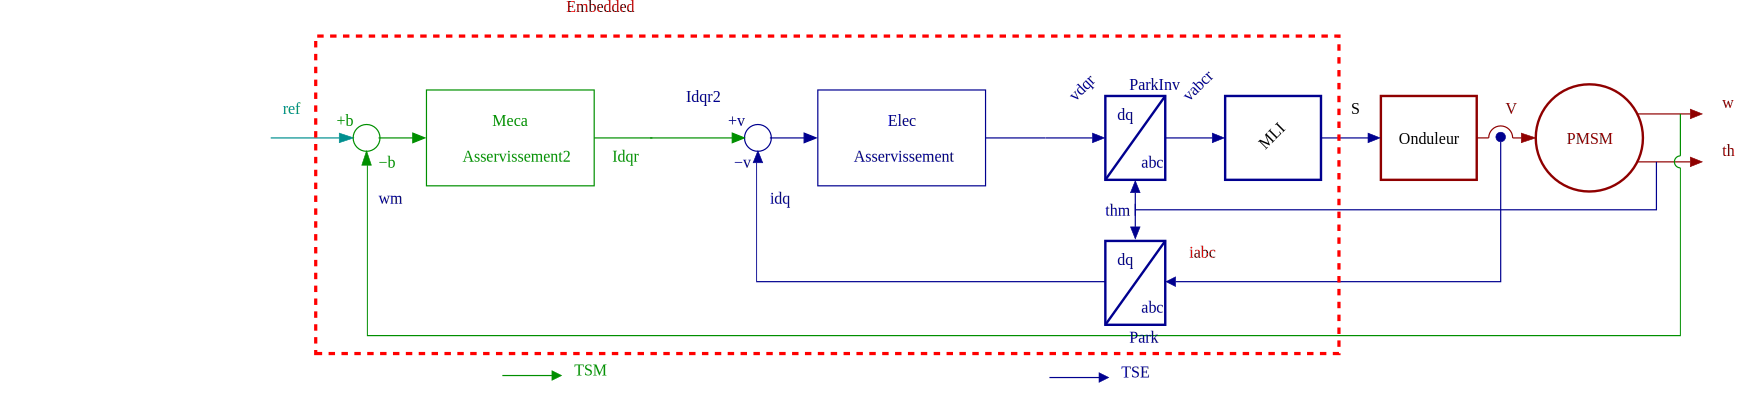
\includegraphics[width = 0.8\textwidth]{pictures/ControlFOC_sanssat.eps}
        \end{psfrags}
\end{figure}

\vspace{0.1cm}
%\begin{columns}[t]
 %   \begin{column}{0.48\textwidth}
        \textbf{Classical approach:}
        \begin{itemize}
            \item Linearize the PMSM model
            \item Second-order  closed-loop dynamics: 
                \begin{itemize}
                    \item Electrical dynamics ($i_d$, $i_q$)
                    \item Mechanical dynamics ($\omega$)
               \end{itemize}
            \item Nested PI controllers
        \end{itemize}
 %   \end{column}

    % \begin{column}{0.48\textwidth}
    %     \textbf{PI characteristics:}
    %     \begin{itemize}
    %           %  \item[\textcolor{blue}{$\checkmark$}] \textcolor{blue}{Hard constraints on poles}
    %             \item[\textcolor{blue}{$\checkmark$}] \textcolor{blue}{Easy to tune $\rightarrow$ hard constraints}
    %             \item[\textcolor{red}{$\times$}] \textcolor{red}{Too restrictive}
    %             \item[\textcolor{red}{$\times$}] \textcolor{red}{No performance optimization}
    %             \item[\textcolor{red}{$\times$}] \textcolor{red}{Difficult to explicitly guarantee robustness}
    %     \end{itemize}
    % \end{column}
%\end{columns}

\end{frame}

\begin{frame}{Embedded control synthesis}{Control synthesis challenges \footnote{ B. Stellato et al., "\textbf{OSQP: an operator splitting solver for quadratic programs}," \textit{Mathematical Programming Computation}, vol. 12, no. 4, pp. 637--672, \textbf{2020}.}}

    \vspace{0.2cm}
    \begin{columns}[t]
        \begin{column}{0.5\textwidth}
            \textbf{PI controllers:}
            \begin{itemize}
                \item[\textcolor{blue}{$\checkmark$}] \textcolor{blue}{Easy to tune: relate $t_r$, overshoot to eigenvalues}
                \item[\textcolor{blue}{$\checkmark$}] \textcolor{blue}{Specific pole locations}
                \item[\textcolor{red}{$\times$}] \textcolor{red}{Too restrictive: no performance optimization}
            \end{itemize}
            \vspace{-0.1cm}
            \centering
            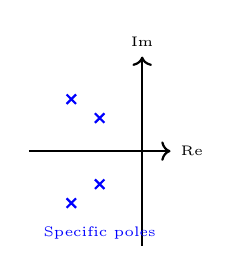
\begin{tikzpicture}[scale=1.2]
                \def\xmin{-1.2cm} \def\xmax{0.3cm}
                \def\ymin{-1.0cm} \def\ymax{1.0cm}

                \draw [thick,->] (\xmin,0) -- (\xmax,0) node [anchor = west]{\tiny $\operatorname{Re}$};
                \draw [thick,->] (0,\ymin) -- (0,\ymax) node [anchor = south]{\tiny $\operatorname{Im}$};

                % Draw crosses for specific eigenvalue locations
                \draw[blue, thick] (-0.5,0.3) -- (-0.4,0.4) (-0.5,0.4) -- (-0.4,0.3);
                \draw[blue, thick] (-0.5,-0.3) -- (-0.4,-0.4) (-0.5,-0.4) -- (-0.4,-0.3);
                \draw[blue, thick] (-0.8,0.5) -- (-0.7,0.6) (-0.8,0.6) -- (-0.7,0.5);
                \draw[blue, thick] (-0.8,-0.5) -- (-0.7,-0.6) (-0.8,-0.6) -- (-0.7,-0.5);

                \node[blue, below] at (-0.45,-0.7) {\tiny Specific poles};
            \end{tikzpicture}
        \end{column}

        \begin{column}{0.5\textwidth}
            \pause
            \textbf{LQR/MPC:}
            \begin{itemize}
                \item[\textcolor{blue}{$\checkmark$}] \textcolor{blue}{Soft constraints $ \min \int_0^\infty (x^\top Q x + u^\top R u) dt$}
                \item[\textcolor{red}{$\times$}] \textcolor{red}{Difficult to tune $Q$, $R$}
                \item[\textcolor{red}{$\times$}] \textcolor{red}{Difficult to explicitly guarantee robustness}
            \end{itemize}
            \vspace{+0.5cm}
                    
        \textbf{Note:} Both methods already embedded in microcontrollers
        \end{column}

    \end{columns}
    %
\end{frame}

\begin{frame}{Embedded control synthesis}{Pole-constrained $\mathcal{H}_2$ control via LMI}
For the same linearized model: 

\vspace{+0.1cm} \textbf{Goal:} \textcolor{blue}{\textbf{Both hard and soft constraints}} + robustness

    \vspace{0.4cm}
    \begin{columns}[t]
    \begin{column}{0.45\textwidth}
        %%%%%%%%% LMI regions figure
    \begin{figure}[]
        \centering
        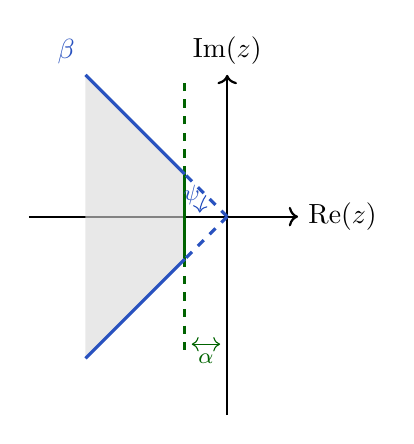
\begin{tikzpicture}[scale=1.8]
    \def\xmin{-1.4cm} \def\xmax{0.5cm}
    \def\ymin{-1.4cm} \def\ymax{1cm}

    \draw [thick,->] (\xmin,0) -- (\xmax,0) node [anchor = west]{$\operatorname{Re}(z)$};
    \draw [thick,->] (0,\ymin) -- (0,\ymax) node [anchor = south]{$\operatorname{Im}(z)$};
    \begin{scope}
      \clip (-1cm,-1cm) rectangle (-0.3cm,1cm);
      \fill[gray!30,opacity=0.6] (-0.3cm,0.3cm) -- (-0.3cm,-0.3cm) -- (-1cm,-1cm) -- (-1cm,1cm) -- cycle;
    \end{scope}
    \draw [darkGreen,line width= 0.4mm] (-0.3cm,-0.3cm) -- (-0.3cm,0.3cm);
    \draw [darkGreen,line width= 0.4mm,dashed] (-0.3cm,0.3cm) -- (-0.3cm,1cm);
    \draw [darkGreen,line width= 0.4mm,dashed] (-0.3cm,-0.3cm) -- (-0.3cm,-1cm);
    \draw [darkBlue,line width= 0.4mm, dashed] (0cm,0cm) -- (-0.3cm,0.3cm);
    \draw [darkBlue,line width= 0.4mm] (-0.3cm,0.3cm) -- (-1cm,1cm);
    \draw [darkBlue,line width= 0.4mm, dashed] (-1cm,1cm) -- (-1cm,1cm) node [pos=1,above left] {$\beta$};
    \draw [darkBlue,line width= 0.4mm, dashed] (0cm,0cm) -- (-0.3cm,-0.3cm);
    \draw [darkBlue,line width= 0.4mm] (-0.3cm,-0.3cm) -- (-1cm,-1cm);
    \draw[->,darkBlue] (-0.15,0.15) arc[start angle=145, end angle=175, radius=0.25cm];
    \node[text=darkBlue] at (-0.25,0.15) {\footnotesize $\psi$};
    \draw[<->,darkGreen] (-0.05,-0.9cm) -- (-0.25cm,-0.9cm) node[midway, below, text=darkGreen] { \footnotesize $\alpha$};
        \end{tikzpicture}
    \end{figure}
    \end{column}

    \begin{column}{0.55\textwidth}
    \textbf{Hard constraints:}    \small{(tuning similar to PI controller)}
    \begin{itemize}
        \item \textcolor{darkGreen}{$\mathbb{D}_\alpha$:} $\alpha$ $\rightarrow$ decay rate 
        \item \textcolor{darkBlue}{$\mathbb{D}_\beta$:} $\beta$ $\rightarrow$ damping ratio
    \end{itemize}


    \vspace{0.3cm}
    \textbf{Soft constraint:}    \small{(similar to LQR/MPC cost)}\\
    \begin{equation*}
        \min \int_0^\infty (x^\top Q x + u^\top R u) dt
    \end{equation*}

    Tuning recommendation: $Q = \mathbf{0}$

    \vspace{0.3cm}
    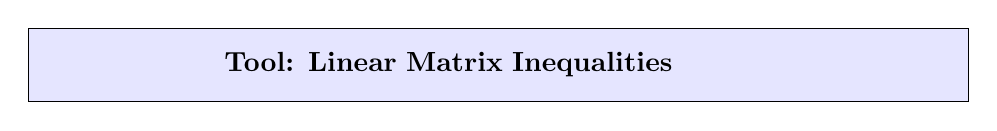
\begin{tikzpicture}
    \node[draw,rectangle,fill=blue!10,text width=0.95\columnwidth,inner sep=6pt]{
    \begin{minipage}{0.9\columnwidth}
    \centering
    \vspace{0.1cm}
    \textbf{Tool: Linear Matrix Inequalities}
    \vspace{0.1cm}
    \end{minipage}};
    \end{tikzpicture}
    \end{column}
    \end{columns}
\end{frame}

\begin{frame}{Embedded control synthesis}{LMI capabilities}

    \begin{columns}[t]
    \begin{column}{0.45\textwidth}
        %%%%%%%%% LMI regions figure with arrow
    \begin{figure}[]
        \centering
        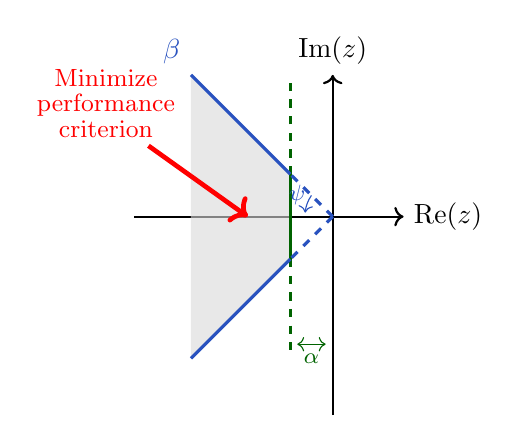
\begin{tikzpicture}[scale=1.8]
    \def\xmin{-1.4cm} \def\xmax{0.5cm}
    \def\ymin{-1.4cm} \def\ymax{1cm}

    \draw [thick,->] (\xmin,0) -- (\xmax,0) node [anchor = west]{$\operatorname{Re}(z)$};
    \draw [thick,->] (0,\ymin) -- (0,\ymax) node [anchor = south]{$\operatorname{Im}(z)$};
    \begin{scope}
      \clip (-1cm,-1cm) rectangle (-0.3cm,1cm);
      \fill[gray!30,opacity=0.6] (-0.3cm,0.3cm) -- (-0.3cm,-0.3cm) -- (-1cm,-1cm) -- (-1cm,1cm) -- cycle;
    \end{scope}
    \draw [darkGreen,line width= 0.4mm] (-0.3cm,-0.3cm) -- (-0.3cm,0.3cm);
    \draw [darkGreen,line width= 0.4mm,dashed] (-0.3cm,0.3cm) -- (-0.3cm,1cm);
    \draw [darkGreen,line width= 0.4mm,dashed] (-0.3cm,-0.3cm) -- (-0.3cm,-1cm);
    \draw [darkBlue,line width= 0.4mm, dashed] (0cm,0cm) -- (-0.3cm,0.3cm);
    \draw [darkBlue,line width= 0.4mm] (-0.3cm,0.3cm) -- (-1cm,1cm);
    \draw [darkBlue,line width= 0.4mm, dashed] (-1cm,1cm) -- (-1cm,1cm) node [pos=1,above left] {$\beta$};
    \draw [darkBlue,line width= 0.4mm, dashed] (0cm,0cm) -- (-0.3cm,-0.3cm);
    \draw [darkBlue,line width= 0.4mm] (-0.3cm,-0.3cm) -- (-1cm,-1cm);
    \draw[->,darkBlue] (-0.15,0.15) arc[start angle=145, end angle=175, radius=0.25cm];
    \node[text=darkBlue] at (-0.25,0.15) {\footnotesize $\psi$};
    \draw[<->,darkGreen] (-0.05,-0.9cm) -- (-0.25cm,-0.9cm) node[midway, below, text=darkGreen] { \footnotesize $\alpha$};

    % Arrow pointing to the gray region from the left
    \draw [->,red,line width=0.6mm] (-1.3cm,0.5cm) -- (-0.6cm,0cm);
    \node[text=red,align=center] at (-1.6cm,0.8cm) {\small Minimize\\[-0.1cm]\small performance\\[-0.1cm]\small criterion};
        \end{tikzpicture}
    \end{figure}
    \end{column}

    \begin{column}{0.55\textwidth}


    %\vspace{0.3cm}
    \textbf{Why LMIs?:}
    %\vspace{0.2cm}
    \begin{itemize}
        \item Convex optimization problems
        \item Hard and soft constraint formulation
        \item Robustness to parametric uncertainty
        \item Anti-windup control design
        \item Formal guarantees via Lyapunov certificates
    \end{itemize}
   
    \end{column}
    \end{columns}

\end{frame}


% \begin{frame}{{Embedded control synthesis}}{PMSM model for pole-constrained $\mathcal{H}_2$ control}
%     %\textbf{LTI state-space form}

%     \begin{columns}[T]
%         \begin{column}{0.5\textwidth}
%             The dynamics of the PMSM is LTI:
%             \begin{align*}
%                 \dot{x}(t) &= Ax(t)+B_u u(t)\\
%                 u(t) &= Kx(t)
%             \end{align*}
%             Augmented with the integral of the tracking error 
%             \begin{eqnarray*}
%                 \varepsilon_{i_d} = \int_{0}^t (i_d^\# - i_d) , d\tau\\
%                 \varepsilon_{\omega} = \int_{0}^t (\omega^\# - \omega) , d\tau\\
%             \end{eqnarray*}
%         \end{column}

%         \begin{column}{0.5\textwidth}
%             \textbf{Control design:}

%             For each subsystem, design $K$ to:
%             \begin{enumerate}
%                 \item Place closed-loop poles in $\mathbb{D}_\alpha \cap \mathbb{D}_\beta$
%                 \begin{itemize}
%                     \item[$\rightarrow$] Transient specifications
%                 \end{itemize}
%                 \item Minimize $\mathcal{H}_2$ norm
%                 \begin{itemize}
%                     \item[$\rightarrow$] Energy efficiency
%                 \end{itemize}
%             \end{enumerate}

%             \vspace{0.3cm}
%             $\Rightarrow$ \textbf{Pole-constrained $\mathcal{H}_2$ synthesis}
%         \end{column}
%     \end{columns}
% \end{frame}


\begin{frame}{Embedded control synthesis}{Pole-constrained $\mathcal{H}_2$ optimization problem}

    % Main content in left minipage
    \begin{minipage}[t]{0.70\textwidth}
    \textbf{Complete LMI formulation:}

    \vspace{-0.2cm}
    \small
    \begin{equation*}
        \min_{X,Y,W,\gamma} \gamma \quad \text{subject to}
    \end{equation*}
    \vspace{-0.3cm}
    \begin{equation*}
        \left.
        \begin{array}{l}
            \begin{bmatrix}
                \langle A\colorbox{SpringGreen}{$X$}+B\colorbox{SpringGreen}{$Y$} \rangle_S  & (*)^\top  \\
                (C_z\colorbox{SpringGreen}{$X$}+D_{z}\colorbox{SpringGreen}{$Y$}) & -I
            \end{bmatrix} \prec 0 \\[3mm]
            \begin{bmatrix}
                \colorbox{SpringGreen}{$W$} & B_w^\top  \\
                B_w & \colorbox{SpringGreen}{$X$}
            \end{bmatrix} \succ 0 \\[3mm]
            \mathrm{trace}(\colorbox{SpringGreen}{$W$}) < \colorbox{SpringGreen}{$\gamma$}
        \end{array}
        \right\} \mathcal{H}_2 \text{ synthesis constraints}
    \end{equation*}
    \vspace{0.2cm}
    \begin{equation*}
        \left.
        \begin{array}{l}
            \langle A\colorbox{SpringGreen}{$X$}+B\colorbox{SpringGreen}{$Y$} \rangle_S  +2 \colorbox{Thistle}{$\alpha$} \colorbox{SpringGreen}{$X$} \prec 0 \\[3mm]
            \begin{bmatrix}
                \colorbox{Thistle}{$\beta$} \langle A\colorbox{SpringGreen}{$X$}+B\colorbox{SpringGreen}{$Y$} \rangle_S  & (*)^\top\\
                (A\colorbox{SpringGreen}{$X$}+B\colorbox{SpringGreen}{$Y$})^\top-(A\colorbox{SpringGreen}{$X$}+B\colorbox{SpringGreen}{$Y$}) & \colorbox{Thistle}{$\beta$} \langle A\colorbox{SpringGreen}{$X$}+B\colorbox{SpringGreen}{$Y$} \rangle_S
            \end{bmatrix} \prec 0
        \end{array}
        \right\} \text{Pole placement constraints}
    \end{equation*}
    \end{minipage}%
    \hfill
    % Small reminder figure in right minipage
    \begin{minipage}[t]{0.27\textwidth}
    \vspace{-1.5cm}
    \hfill
    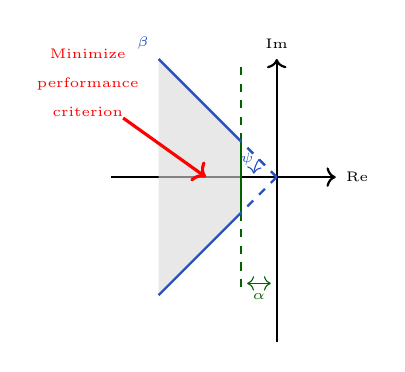
\begin{tikzpicture}[scale=1.5]
    \def\xmin{-1.4cm} \def\xmax{0.5cm}
    \def\ymin{-1.4cm} \def\ymax{1cm}

    \draw [thick,->] (\xmin,0) -- (\xmax,0) node [anchor = west]{\tiny $\operatorname{Re}$};
    \draw [thick,->] (0,\ymin) -- (0,\ymax) node [anchor = south]{\tiny $\operatorname{Im}$};
    \begin{scope}
      \clip (-1cm,-1cm) rectangle (-0.3cm,1cm);
      \fill[gray!30,opacity=0.6] (-0.3cm,0.3cm) -- (-0.3cm,-0.3cm) -- (-1cm,-1cm) -- (-1cm,1cm) -- cycle;
    \end{scope}
    \draw [darkGreen,line width= 0.3mm] (-0.3cm,-0.3cm) -- (-0.3cm,0.3cm);
    \draw [darkGreen,line width= 0.3mm,dashed] (-0.3cm,0.3cm) -- (-0.3cm,1cm);
    \draw [darkGreen,line width= 0.3mm,dashed] (-0.3cm,-0.3cm) -- (-0.3cm,-1cm);
    \draw [darkBlue,line width= 0.3mm, dashed] (0cm,0cm) -- (-0.3cm,0.3cm);
    \draw [darkBlue,line width= 0.3mm] (-0.3cm,0.3cm) -- (-1cm,1cm);
    \draw [darkBlue,line width= 0.3mm, dashed] (0cm,0cm) -- (-0.3cm,-0.3cm);
    \draw [darkBlue,line width= 0.3mm] (-0.3cm,-0.3cm) -- (-1cm,-1cm);
    % Add labels
    \draw[->,darkBlue] (-0.15,0.15) arc[start angle=145, end angle=175, radius=0.25cm];
    \node[text=darkBlue] at (-0.25,0.15) {\tiny $\psi$};
    \draw[<->,darkGreen] (-0.05,-0.9cm) -- (-0.25cm,-0.9cm) node[midway, below, text=darkGreen] {\tiny $\alpha$};
    \node[text=darkBlue] at (-1cm,1cm) [above left] {\tiny $\beta$};
    % Arrow pointing to the gray region from the left
    \draw [->,red,line width=0.4mm] (-1.3cm,0.5cm) -- (-0.6cm,0cm);
    \node[text=red,align=center] at (-1.6cm,0.8cm) {\tiny Minimize\\[-0.05cm]\tiny performance\\[-0.05cm]\tiny criterion};
    \end{tikzpicture}
    \end{minipage}

\end{frame}
\begin{frame}{Embedded control synthesis}

          % \only<1>{
            
            \begin{figure}
                \centering
                \includegraphics[width=0.7\columnwidth]{pictures/PMSM_test_bench.eps}
            \end{figure}
           %} 
        %    \only<2>{
        %     \vspace{-0.5cm}
        %     \begin{figure}
        %         \centering
        %         \includegraphics[width=0.75\columnwidth]{pictures/combined.eps}
        %     \end{figure}    
        %    }
\end{frame}

\begin{frame}{Embedded control synthesis}{How to solve an LMI problem?}
    \begin{columns}
       \vspace{-1cm} \begin{column}{0.45\textwidth}
            \textbf{Solution methodology:}
            \begin{enumerate}
                \only<1->{\item \textbf{Parametrization}}\only<2>{ : express decision variables as linear combinations of basis matrices
                    \begin{equation*} \label{eq:ParamX}
                         X=  X(\xi) = \sum_{i=1}^{n(n+1)/2} \xi_i X_i
                    \end{equation*}}
                  \only<2->{  The LMI constraints become:
                    \begin{equation*} \label{eq:DefinitionLMI}
                        F(\xi) = F_0 +\sum^{\mu+1}_{i=1}\xi_i F_i \succ 0
                    \end{equation*} }
                \item\only<1->{\textbf{Feasibility}}\only<3>{: find an initial feasible point 
                \begin{equation*} \label{eq:FeasibilityProblem}
                    \begin{aligned}
                    &\underset{\xi= [\xi_e,\gamma],\lambda}{\mathrm{min}} \ \lambda \ \mathrm{s.t.} \\
                    & F(\xi)+\lambda I \succ 0  
                    \end{aligned}
                \end{equation*}}
                \item \only<1->{\textbf{Optimization}}\only<4>{ Minimize the objective function
                 \begin{equation*}\label{eq:optimizationProblem}
                    \begin{aligned}
                    &\underset{\xi= [\xi_e,\gamma],\lambda}{\mathrm{min}} \ \gamma \ \mathrm{s.t.} \\
                    & F(\xi)+\lambda I \succ 0 
                    %& -\varepsilon-\lambda \geq 0 
                    \end{aligned}
                \end{equation*}}
            \end{enumerate}
        \end{column}

        \begin{column}{0.55\textwidth}

            \begin{figure}
                \centering
                \includegraphics[width=0.95\columnwidth]{pictures/combined.eps}
            \end{figure}
        \end{column}
    \end{columns}
\end{frame}

% \begin{frame}{Embedded control synthesis}{Embedded LMI solver}
%     \centering
%     \includegraphics[trim={0cm 0cm 0cm 0cm},clip,width=0.9\framewidth]{pictures/online_offline_ink_trajec_full1.eps}
% \end{frame}

\begin{frame}{Practical implementation: Real-time scheduler}
        \textbf{Hardware platforms:}
    \begin{itemize}
        %\item ATSAME54P20A microcontroller (120 MHz, 256 KB RAM, $\sim$\$5)
        \item dsPIC33AK512 DSC $\sim$\$3
    \end{itemize}
    \textbf{Two concurrent tasks:}
    \vspace{0.2cm}

            \begin{figure}
            \begin{center}
                \def\textsize{.8}
                \psfrag{Algo}[c][c][1]{\color{Blue4}Control}
                \psfrag{Control}[c][c][1]{\color{Blue4}Control}
                \psfrag{iabc}[c][c][\textsize]{\color{Blue4}$i_{abc}$}
                \psfrag{idq}[c][c][\textsize]{\color{Blue4}$i_{dq}$}
                \psfrag{vabcr}[c][c][\textsize]{\color{Blue4}$v_{abc}^\#$}
                \psfrag{vdqr}[c][c][\textsize]{\color{Blue4}$v_{dq}^\#$}
                \psfrag{dq}[c][c][.5]{\color{Blue4}${dq}$}
                \psfrag{abc}[c][c][.5]{\color{Blue4}${abc}\quad$}
                \psfrag{S}[c][c][\textsize]{\color{Blue4}$S_{abc}$}
                \psfrag{MLI}[c][c][\textsize]{\color{Blue4}Mod}
                \psfrag{ParkInv}[c][c][.5]{}
                \psfrag{Park}[c][c][.5]{}
                \psfrag{TS1}[l][c][.6]{\color{Blue4}Higher priority $\approx20$kHz}
                % Reference generation (cyan) - lower priority optimization
                \psfrag{Vr}[c][c][\textsize]{\color{Cyan4}$\rho^\#$}
                \psfrag{ref}[c][c][\textsize]{\color{Cyan4}$\omega^\#$}
                \psfrag{ref2}[c][c][\textsize]{\color{Cyan4}$i_d^\#$}
                \psfrag{ref3}[c][c][\textsize]{\color{Cyan4}$\omega^\#$}
                \psfrag{ref4}[c][c][\textsize]{\color{Cyan4}$i_q$}
                \psfrag{ref5}[c][c][\textsize]{\color{Magenta4} Specification}
                \psfrag{ref6}[c][c][\textsize]{\color{Magenta4} Model}
                \psfrag{Reference}[c][c][\textsize]{\color{Cyan4}Trajectory}
                \psfrag{calculation}[c][c][\textsize]{\color{Cyan4}generation}
                \psfrag{TS2}[l][c][.6]{\color{Cyan4}Lower priority $\approx1$kHz}
                % Embedded synthesis (magenta) - idle task
                \psfrag{Emb}[c][c][\textsize]{\color{Magenta4}Embedded}
                \psfrag{Synt}[c][c][\textsize]{\color{Magenta4}synthesis}
                \psfrag{K}[c][c][\textsize]{\color{Magenta4}K}
                \psfrag{TS3}[l][c][.6]{\color{Magenta4}Idle task}
                % Physical system (red) - PMSM and measurements
                \psfrag{Onduleur}[c][c][\textsize]{\color{Red4}Inverter}
                \psfrag{PMSM}[c][c][\textsize]{\color{Red4}PMSM}
                \psfrag{V}[c][c][\textsize]{\color{Red4}$v_{abc}$}
                \psfrag{th}[c][c][\textsize]{\color{Red4}$\theta$}
                \psfrag{w}[c][c][\textsize]{\color{Red4}$\omega$}
                \psfrag{thm}[c][c][\textsize]{\color{Red4}$\theta$}
                \psfrag{wm}[c][c][\textsize]{\color{Red4}$\omega$}
                \psfrag{Embedded}[l][c][.7]{\color{red}Embedded code}
                \includegraphics[width = .9\textwidth]{pictures/AdvancedControl.eps}
            \end{center}
        \label{fig:AdvencedControlForElectricalMotor}
        \end{figure}
        
   
\end{frame}

\begin{frame}{Embedded control synthesis}{Rate-monotonic scheduler}
    \textbf{Multi-rate scheduling:} High-priority tasks preempt low-priority tasks

    \vspace{0.3cm}
         \begin{figure}
        \centering
        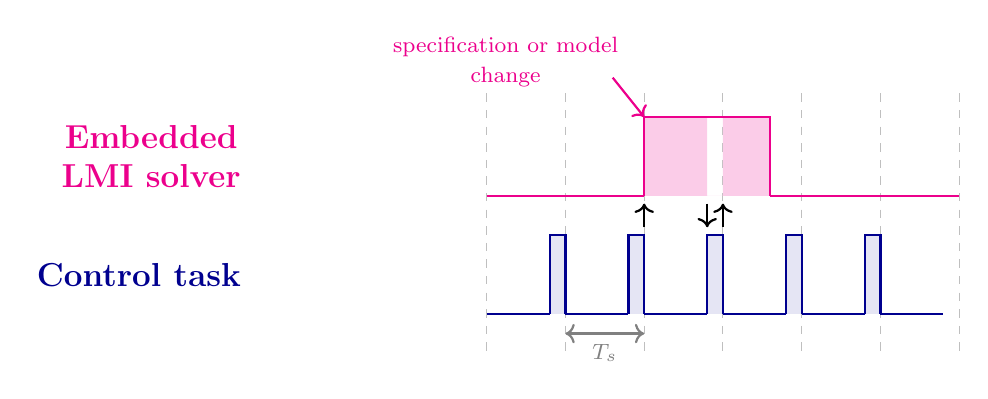
\begin{tikzpicture}[xscale=2, yscale=1, every node/.style={font=\small}]
            % Time line
            \foreach \x in {1,...,4} {
                \draw[gray!50, dashed] (\x,1.3) -- (\x,-2);
            }
            % Gray vertical lines at control task falling edges
            \foreach \x in {1.5,2.0,2.5,3.0,3.5} {
                \draw[gray!50, dashed] (\x,1.3) -- (\x,-2);
            }
            % Double arrow showing sampling period
            \draw[<->,thick,gray] (1.5,-1.75) -- (2.0,-1.75) node[midway,below,gray] {\footnotesize $T_s$};
            \fill[magenta!20] (2,0) -- (2,1) -- (2.4,1) -- (2.4,0) --(2.5,0)--(2.5,1)--(2.8,1)--(2.8,0);
             %%%%%%%%%%%%%%% Pulse high blue
            \foreach \x in {2} {
                \draw[draw= magenta, thick] (\x,0) -- (\x,1) -- (\x+0.8,1) -- (\x+0.8,0);
            }
            %%%%%%%%%%%%%%%% Pulse low blue
            \draw[magenta,thick] (1,0) -- (2,0);
            \draw[magenta,thick] (2.8,0)--(4,0) ;
            \node[align=center, left, magenta, font=\large\bfseries] at (-0.5,0.5) {Embedded \\ LMI solver};
            %%%%%%%%%%%%%%%% Pulse  high red
            \foreach \x in {1.4,1.9,2.4,...,3.4} {
                \draw[thick, blue4, fill=blue4!10] (\x,-1.5) -- (\x,-0.5) -- (\x+0.1,-0.5)-- (\x+0.1,-1.5);
           }
           %%%%%%%%%%%%%%%%% Pulse low red
            \foreach \x in {1,1.5,...,3.5} {
                    \draw[thick, blue4]  (\x,-1.5) -- (\x+0.4,-1.5);
            }
            \node[left, blue4, align=center, font=\large\bfseries] at (-0.5,-1) {Control task};
            %%%%%%%%%%%%%%%%% vertical arrows to explain
            \draw[->,thick] (2,-0.4)--(2,0-0.1);
            \draw[->,thick] (2.4,-0.1) --(2.4,-0.4);
            \draw[->,thick] (2.5,-0.4) --(2.5,-0.1);
            %%%%%%%%%%%%%%%%% Arrow pointing to first rising edge
            \draw[->,thick,magenta] (1.8,1.5) -- (2,1) node[midway,above left,magenta,align=center] {\footnotesize specification or model \\ \footnotesize  change};
            %%%%%%%%%%%%%%%%% Time line
            %\draw[->, thick] (0.5,-1.9) --(4.5,-1.9) node [right, align= center] {time} ;
        \end{tikzpicture}
    \end{figure}

    \vspace{-0.2cm}
    \begin{itemize}
        \item \textcolor{blue4}{High-priority task (20 kHz)}: Control loop runs deterministically
        \item \textcolor{magenta}{Low-priority task (idle)}: LMI solver interrupted when needed
    \end{itemize}
 \end{frame}
% \begin{frame}{Embedded control synthesis}{Experimental validation}
%             \begin{figure}[h!]
%                 \centering 
%                 \centerline{\includegraphics[width=0.7\textwidth]{pictures/PMSM_test_bench.eps}}
%             \end{figure}
% \end{frame}
\begin{frame}{Embedded control synthesis}{Experimental validation}
 \begin{columns}
        \begin{column}{0.5\textwidth}
            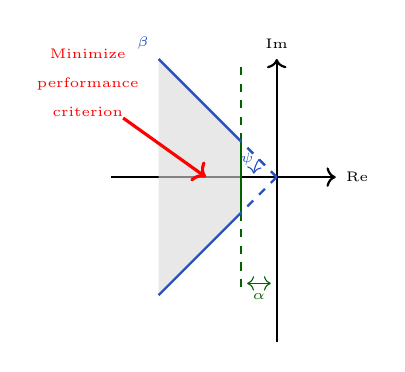
\begin{tikzpicture}[scale=1.5]
    \def\xmin{-1.4cm} \def\xmax{0.5cm}
    \def\ymin{-1.4cm} \def\ymax{1cm}

    \draw [thick,->] (\xmin,0) -- (\xmax,0) node [anchor = west]{\tiny $\operatorname{Re}$};
    \draw [thick,->] (0,\ymin) -- (0,\ymax) node [anchor = south]{\tiny $\operatorname{Im}$};
    \begin{scope}
      \clip (-1cm,-1cm) rectangle (-0.3cm,1cm);
      \fill[gray!30,opacity=0.6] (-0.3cm,0.3cm) -- (-0.3cm,-0.3cm) -- (-1cm,-1cm) -- (-1cm,1cm) -- cycle;
    \end{scope}
    \draw [darkGreen,line width= 0.3mm] (-0.3cm,-0.3cm) -- (-0.3cm,0.3cm);
    \draw [darkGreen,line width= 0.3mm,dashed] (-0.3cm,0.3cm) -- (-0.3cm,1cm);
    \draw [darkGreen,line width= 0.3mm,dashed] (-0.3cm,-0.3cm) -- (-0.3cm,-1cm);
    \draw [darkBlue,line width= 0.3mm, dashed] (0cm,0cm) -- (-0.3cm,0.3cm);
    \draw [darkBlue,line width= 0.3mm] (-0.3cm,0.3cm) -- (-1cm,1cm);
    \draw [darkBlue,line width= 0.3mm, dashed] (0cm,0cm) -- (-0.3cm,-0.3cm);
    \draw [darkBlue,line width= 0.3mm] (-0.3cm,-0.3cm) -- (-1cm,-1cm);
    % Add labels
    \draw[->,darkBlue] (-0.15,0.15) arc[start angle=145, end angle=175, radius=0.25cm];
    \node[text=darkBlue] at (-0.25,0.15) {\tiny $\psi$};
    \draw[<->,darkGreen] (-0.05,-0.9cm) -- (-0.25cm,-0.9cm) node[midway, below, text=darkGreen] {\tiny $\alpha$};
    \node[text=darkBlue] at (-1cm,1cm) [above left] {\tiny $\beta$};
    % Arrow pointing to the gray region from the left
    \draw [->,red,line width=0.4mm] (-1.3cm,0.5cm) -- (-0.6cm,0cm);
    \node[text=red,align=center] at (-1.6cm,0.8cm) {\tiny Minimize\\[-0.05cm]\tiny performance\\[-0.05cm]\tiny criterion};
    \end{tikzpicture}
    \end{column}
    \begin{column}{0.5\textwidth}
        
    
            \begin{figure}[h!]
                \centering 
                \centerline{\includegraphics[width=1\columnwidth]{pictures/alpha_step_AK512_1.eps}}
            \end{figure}
\end{column}
\end{columns}
        \end{frame}


\begin{frame}{Embedded control synthesis}{Experimental validation (No laod)}
    \begin{columns}
        \begin{column}{0.4\textwidth}
            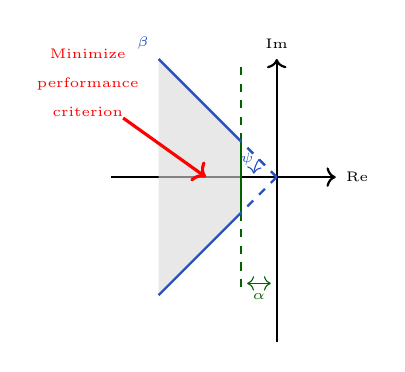
\begin{tikzpicture}[scale=1.5]
    \def\xmin{-1.4cm} \def\xmax{0.5cm}
    \def\ymin{-1.4cm} \def\ymax{1cm}

    \draw [thick,->] (\xmin,0) -- (\xmax,0) node [anchor = west]{\tiny $\operatorname{Re}$};
    \draw [thick,->] (0,\ymin) -- (0,\ymax) node [anchor = south]{\tiny $\operatorname{Im}$};
    \begin{scope}
      \clip (-1cm,-1cm) rectangle (-0.3cm,1cm);
      \fill[gray!30,opacity=0.6] (-0.3cm,0.3cm) -- (-0.3cm,-0.3cm) -- (-1cm,-1cm) -- (-1cm,1cm) -- cycle;
    \end{scope}
    \draw [darkGreen,line width= 0.3mm] (-0.3cm,-0.3cm) -- (-0.3cm,0.3cm);
    \draw [darkGreen,line width= 0.3mm,dashed] (-0.3cm,0.3cm) -- (-0.3cm,1cm);
    \draw [darkGreen,line width= 0.3mm,dashed] (-0.3cm,-0.3cm) -- (-0.3cm,-1cm);
    \draw [darkBlue,line width= 0.3mm, dashed] (0cm,0cm) -- (-0.3cm,0.3cm);
    \draw [darkBlue,line width= 0.3mm] (-0.3cm,0.3cm) -- (-1cm,1cm);
    \draw [darkBlue,line width= 0.3mm, dashed] (0cm,0cm) -- (-0.3cm,-0.3cm);
    \draw [darkBlue,line width= 0.3mm] (-0.3cm,-0.3cm) -- (-1cm,-1cm);
    % Add labels
    \draw[->,darkBlue] (-0.15,0.15) arc[start angle=145, end angle=175, radius=0.25cm];
    \node[text=darkBlue] at (-0.25,0.15) {\tiny $\psi$};
    \draw[<->,darkGreen] (-0.05,-0.9cm) -- (-0.25cm,-0.9cm) node[midway, below, text=darkGreen] {\tiny $\alpha$};
    \node[text=darkBlue] at (-1cm,1cm) [above left] {\tiny $\beta$};
    % Arrow pointing to the gray region from the left
    \draw [->,red,line width=0.4mm] (-1.3cm,0.5cm) -- (-0.6cm,0cm);
    \node[text=red,align=center] at (-1.6cm,0.8cm) {\tiny Minimize\\[-0.05cm]\tiny performance\\[-0.05cm]\tiny criterion};
    \end{tikzpicture}
    \end{column}
    
    \begin{column}{0.6\textwidth}
           \begin{figure}[H]
            \centering
             \centerline{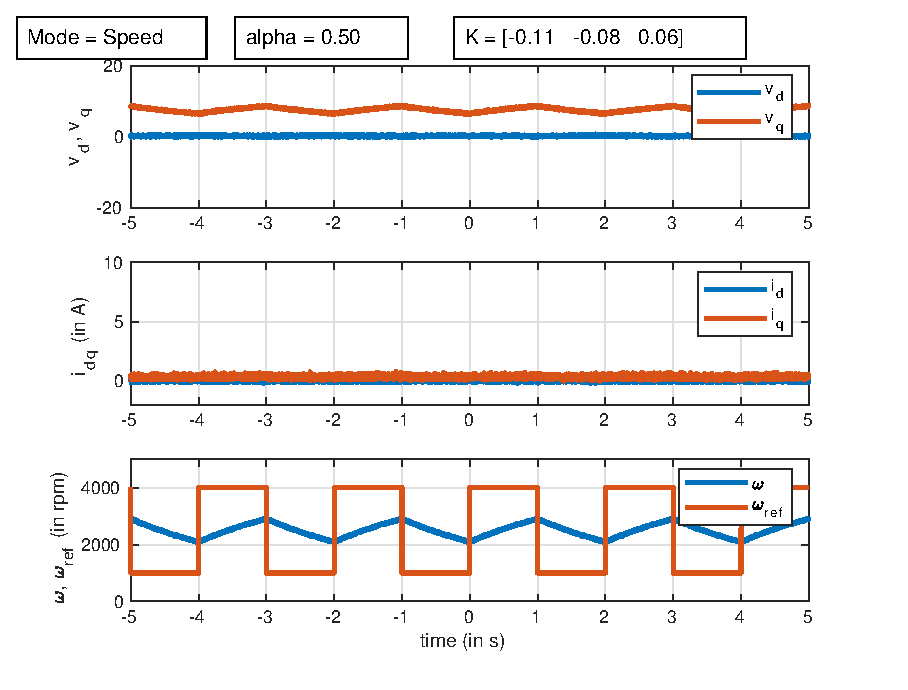
\includegraphics[width=0.7\framewidth]{pictures/expeSolver/LMI1.eps}}
             \caption{Experimental validation for $\alpha = 0.5$}
\end{figure}   
    \end{column}
    \end{columns}
\end{frame}
% \begin{frame}{Embedded control synthesis}{Experimental validation}
%     \begin{figure}[H]
%   \centering
%   \centerline{\includegraphics[width=0.7\framewidth]{pictures/expeSolver/LMI3.eps}}
%   \caption{Experiment validation for $\alpha = 5.80$.}
%   \label{fig:alpha5}
% \end{figure}
% \end{frame}

% \begin{frame}{Embedded control synthesis}{Experimental validation}
%     \begin{figure}[H]
%   \centering
%   \centerline{\includegraphics[width=0.7\framewidth]{pictures/expeSolver/LMI4.eps}}
%   \caption{Experiment validation for $\alpha = 25.87$}
%   \label{fig:alpha25}
% \end{figure}
% \end{frame}

\begin{frame}{Embedded control synthesis}{Experimental validation (no load)}
        \begin{columns}
        \begin{column}{0.4\textwidth}
            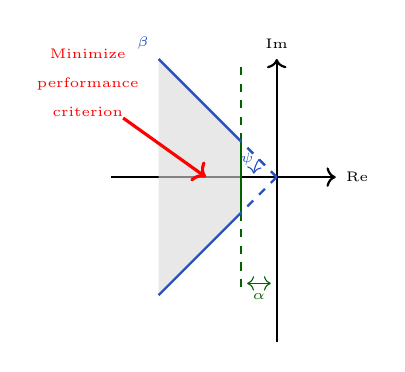
\begin{tikzpicture}[scale=1.5]
    \def\xmin{-1.4cm} \def\xmax{0.5cm}
    \def\ymin{-1.4cm} \def\ymax{1cm}

    \draw [thick,->] (\xmin,0) -- (\xmax,0) node [anchor = west]{\tiny $\operatorname{Re}$};
    \draw [thick,->] (0,\ymin) -- (0,\ymax) node [anchor = south]{\tiny $\operatorname{Im}$};
    \begin{scope}
      \clip (-1cm,-1cm) rectangle (-0.3cm,1cm);
      \fill[gray!30,opacity=0.6] (-0.3cm,0.3cm) -- (-0.3cm,-0.3cm) -- (-1cm,-1cm) -- (-1cm,1cm) -- cycle;
    \end{scope}
    \draw [darkGreen,line width= 0.3mm] (-0.3cm,-0.3cm) -- (-0.3cm,0.3cm);
    \draw [darkGreen,line width= 0.3mm,dashed] (-0.3cm,0.3cm) -- (-0.3cm,1cm);
    \draw [darkGreen,line width= 0.3mm,dashed] (-0.3cm,-0.3cm) -- (-0.3cm,-1cm);
    \draw [darkBlue,line width= 0.3mm, dashed] (0cm,0cm) -- (-0.3cm,0.3cm);
    \draw [darkBlue,line width= 0.3mm] (-0.3cm,0.3cm) -- (-1cm,1cm);
    \draw [darkBlue,line width= 0.3mm, dashed] (0cm,0cm) -- (-0.3cm,-0.3cm);
    \draw [darkBlue,line width= 0.3mm] (-0.3cm,-0.3cm) -- (-1cm,-1cm);
    % Add labels
    \draw[->,darkBlue] (-0.15,0.15) arc[start angle=145, end angle=175, radius=0.25cm];
    \node[text=darkBlue] at (-0.25,0.15) {\tiny $\psi$};
    \draw[<->,darkGreen] (-0.05,-0.9cm) -- (-0.25cm,-0.9cm) node[midway, below, text=darkGreen] {\tiny $\alpha$};
    \node[text=darkBlue] at (-1cm,1cm) [above left] {\tiny $\beta$};
    % Arrow pointing to the gray region from the left
    \draw [->,red,line width=0.4mm] (-1.3cm,0.5cm) -- (-0.6cm,0cm);
    \node[text=red,align=center] at (-1.6cm,0.8cm) {\tiny Minimize\\[-0.05cm]\tiny performance\\[-0.05cm]\tiny criterion};
    \end{tikzpicture}
    \end{column}
    
    \begin{column}{0.6\textwidth}
    
    \begin{figure}[H]
  \centering
  \centerline{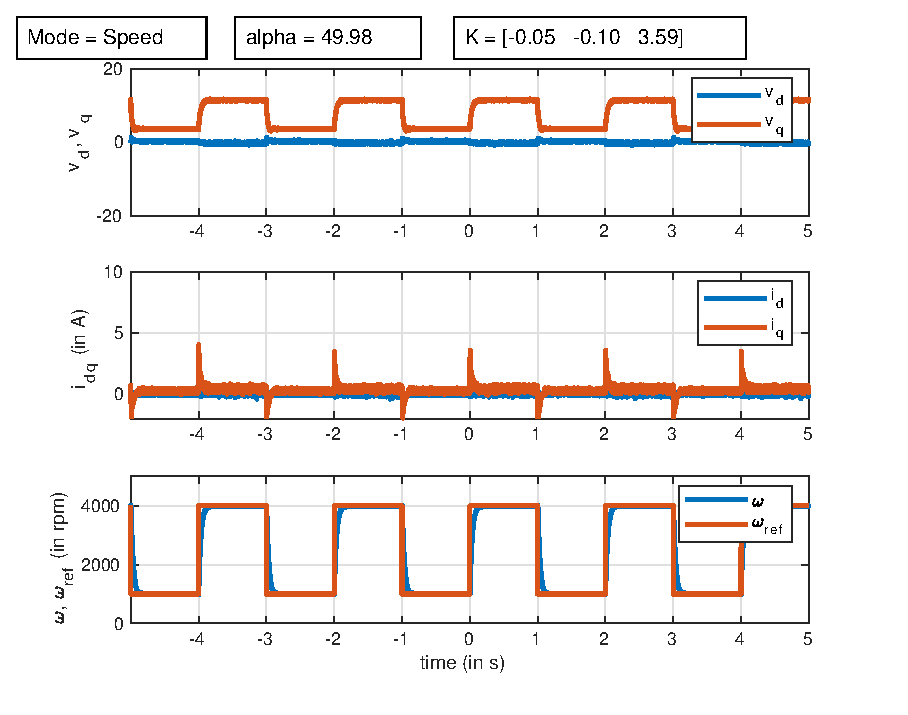
\includegraphics[width=0.7\framewidth]{pictures/expeSolver/LMI5.eps}}
  \caption{Experimental validation for $\alpha = 49.98$}
  \label{fig:alpha50}
  \end{figure}
    \end{column}
\end{columns}

\end{frame}

\begin{frame}{Embedded control synthesis}{Control performance: Results summary}
    \textbf{Experimental validation confirms:}

    \vspace{0.3cm}
    \begin{itemize}
        \item[$\checkmark$] \textbf{Solver operates correctly as idle task}
         \item[$\checkmark$] \textbf{No need for external intervention}

        \item[$\checkmark$] \textbf{Computational time for this application is 0.3 s}
        \begin{itemize}
            \item Dependent on the hardware, the size of the problem, or on the low priority task load.
        \end{itemize}
    \end{itemize}
    \vspace{+0.1cm}
    \textbf{Remark:}
    \begin{itemize}
        \item the LMI solver is generic
    \end{itemize} 

    \vspace{0.3cm}
    \begin{center}
    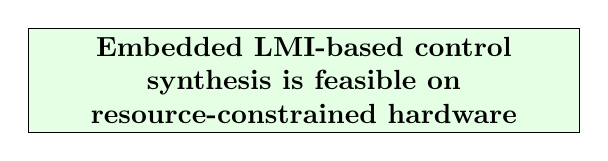
\begin{tikzpicture}
        \node[draw, rectangle, fill=green!10, minimum width=7cm, minimum height=0.8cm] {
            \begin{minipage}{6.5cm}
                \centering
                \textbf{Embedded LMI-based control synthesis is feasible on resource-constrained hardware}
            \end{minipage}
        };
    \end{tikzpicture}
    \end{center}
\end{frame}



%%%%%%%%%%%%%%%%%%%%%%%%%%%%%%%%%%%%%%%%%%%%%%%%%%%%%%%%%%%%%%%%%%%%%%%%%%
\begin{frame}{Outline}
        \textbf{Objectives:}
    \vspace{0.2cm}
    \begin{enumerate}
        \item[\textcolor{darkgray}{\textbf{1.}}] \textcolor{darkgray}{\textbf{What are the optimal currents $i_d^\#$, $i_q^\#$ to produce desired torque $\tau$ and speed $\omega$ ?}}
        \item[\textcolor{darkgray}{\textbf{2.}}] \textcolor{darkgray}{\textbf{Embedded closed-loop control synthesis}}
        \item[\textcolor{Blue4}{\textbf{3.}}] \textcolor{Blue4}{\textbf{New control approaches}}
    \end{enumerate}
        \begin{figure}
            \begin{center}
                \def\textsize{.8}
                \psfrag{Algo}[c][c][1]{\color{Blue4}Control}
                \psfrag{Control}[c][c][1]{\color{Blue4}Control}
                \psfrag{iabc}[c][c][\textsize]{\color{Blue4}$i_{abc}$}
                \psfrag{idq}[c][c][\textsize]{\color{Blue4}$i_{dq}$}
                \psfrag{vabcr}[c][c][\textsize]{\color{Blue4}$v_{abc}^\#$}
                \psfrag{vdqr}[c][c][\textsize]{\color{Blue4}$v_{dq}^\#$}
                \psfrag{dq}[c][c][.5]{\color{Blue4}${dq}$}
                \psfrag{abc}[c][c][.5]{\color{Blue4}${abc}\quad$}
                \psfrag{S}[c][c][\textsize]{\color{Blue4}$S_{abc}$}
                \psfrag{MLI}[c][c][\textsize]{\color{Blue4}Mod}
                \psfrag{ParkInv}[c][c][.5]{}
                \psfrag{Park}[c][c][.5]{}
                \psfrag{TS1}[l][c][.6]{\color{Blue4}Higher priority $\approx20$kHz}
                % Reference generation (cyan) - lower priority optimization
                \psfrag{Vr}[c][c][\textsize]{\color{Cyan4}$\rho^\#$}
                \psfrag{ref}[c][c][\textsize]{\color{gray}$\omega^\#$}
                \psfrag{ref2}[c][c][\textsize]{\color{gray}$i_d^\#$}
                \psfrag{ref3}[c][c][\textsize]{\color{gray}$\omega^\#$}
                \psfrag{ref4}[c][c][\textsize]{\color{Cyan4}$i_q$}
                \psfrag{ref5}[c][c][\textsize]{\color{gray} Specification}
                \psfrag{ref6}[c][c][\textsize]{\color{gray} Model}
                \psfrag{Reference}[c][c][\textsize]{\color{gray}Trajectory}
                \psfrag{calculation}[c][c][\textsize]{\color{gray}generation}
                \psfrag{TS2}[l][c][.6]{\color{Cyan4}Lower priority $\approx1$kHz}
                % Embedded synthesis (magenta) - idle task
                \psfrag{Emb}[c][c][\textsize]{\color{gray}Embedded}
                \psfrag{Synt}[c][c][\textsize]{\color{gray}synthesis}
                \psfrag{K}[c][c][\textsize]{\color{gray}K}
                \psfrag{TS3}[l][c][.6]{\color{Magenta4}Idle task}
                % Physical system (red) - PMSM and measurements
                \psfrag{Onduleur}[c][c][\textsize]{\color{Red4}Inverter}
                \psfrag{PMSM}[c][c][\textsize]{\color{Red4}PMSM}
                \psfrag{V}[c][c][\textsize]{\color{Red4}$v_{abc}$}
                \psfrag{th}[c][c][\textsize]{\color{Red4}$\theta$}
                \psfrag{w}[c][c][\textsize]{\color{Red4}$\omega$}
                \psfrag{thm}[c][c][\textsize]{\color{Red4}$\theta$}
                \psfrag{wm}[c][c][\textsize]{\color{Red4}$\omega$}
                \psfrag{Embedded}[l][c][.7]{\color{red}Embedded code}
                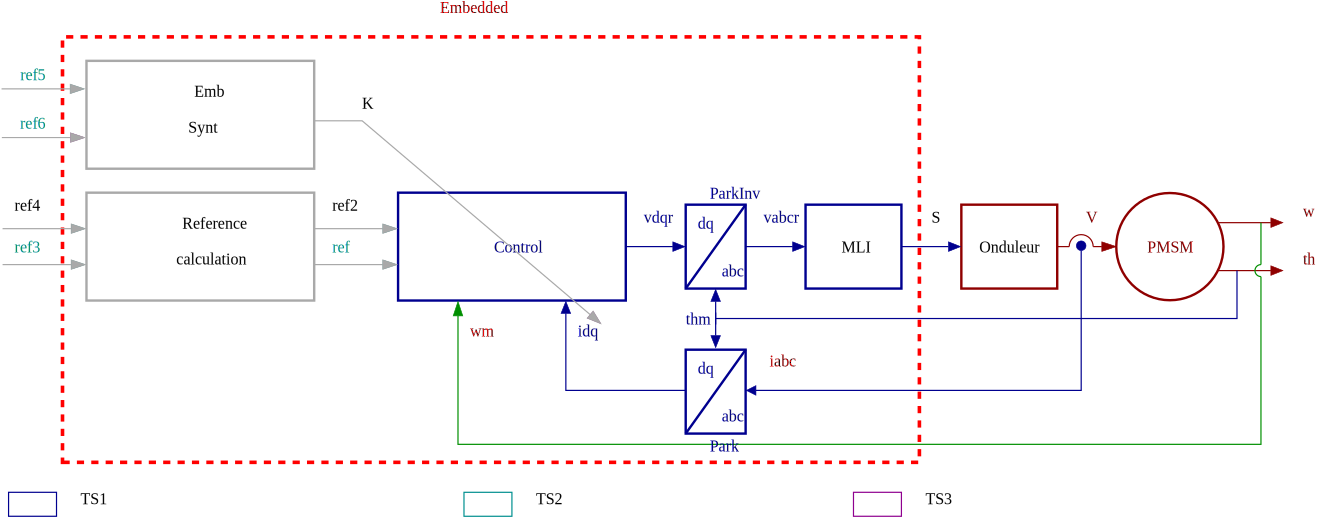
\includegraphics[width = .9\textwidth]{pictures/AdvancedControl_control.eps}
            \end{center}
        \label{fig:AdvencedControlForElectricalMotor}
        \end{figure}
\end{frame}



% ========================================
% Section 3: Linear Parameter Varying Control
% ========================================
\section{Linear parameter varying control}
\begin{frame}{Linear parameter varying control}{Classical approach}
\begin{columns}[T]
    \begin{column}{0.48\textwidth}
        \textbf{Nonlinear PMSM dynamics:}
            \begin{align*}
        L_d \frac{di_d}{dt} &= v_d - Ri_d \textcolor{red}{+p L_q\omega i_q} \\
        L_q\frac{di_q}{dt} &= v_q -Ri_q \textcolor{red}{-pL_d\omega i_d} -p \phi_f\omega
            \end{align*}

            \pause
            \vspace{0.2cm}
            \textbf{Feedback linearization:}
            \begin{equation*}
                \begin{cases}
                    v_d = u_d -pL_q\omega i_q\\
                    v_q = u_q +pL_d\omega i_d
                \end{cases}
            \end{equation*}
            \pause
    \end{column}
    \begin{column}{0.48\textwidth}
        \textbf{Linearized system:}
            \begin{equation*}
              \dot{x}= A x +B_u u
            \end{equation*}

            \pause
            \vspace{0.2cm}
            \textbf{Augmented state:}
            \begin{align*}
                \varepsilon_{i_d} &= \int_{0}^t (i_d^\# - i_d) d\tau\\
                \varepsilon_{i_q} &= \int_{0}^t (i_q^\# - i_q) d\tau
            \end{align*}

        \pause
        \vspace{0.2cm}
            \textbf{PI control law:}
            \begin{equation*}
                u = K x
            \end{equation*}
    \end{column}
\end{columns}
\end{frame}

\begin{frame}{Linear parameter varying control}{Proposed LPV approach}
\begin{columns}[T]
    \begin{column}{0.48\textwidth}
        \textbf{Nonlinear PMSM dynamics:}
            \begin{align*}
        L_d \frac{di_d}{dt} &= v_d - Ri_d \textcolor{red}{+p L_q\omega i_q} \\
        L_q \frac{di_q}{dt} &= v_q -Ri_q \textcolor{red}{-pL_d\omega i_d} -p \phi_f\omega
            \end{align*}

            \vspace{0.3cm}
            \textbf{Classical approach:}
            \begin{equation*}
                \xcancel{\begin{cases}
                    v_d = u_d -pL_q\omega i_q\\
                    v_q = u_q +pL_d\omega i_d
                \end{cases}}
            \end{equation*}
            \pause
    \end{column}
    \begin{column}{0.48\textwidth}
        \textbf{LPV model:}
            \begin{align*}
               \dot{x} &= A(\omega)x +B_u u\\
               \omega &\in \left[ \omega_{\min},\, \omega_{\max} \right]
            \end{align*}

            \pause
            \vspace{0.2cm}
            \textbf{Augmented state:}
            \begin{equation*}
                x = \begin{bmatrix}
                i_d & i_q & \varepsilon_{i_d}& \varepsilon_{i_q}
            \end{bmatrix}^\top
            \end{equation*}

            \pause
            \vspace{0.2cm}
            \textbf{Parameter dependant control:}
            \begin{equation*}
                v_{dq} =  K (\omega)x
            \end{equation*}
    \end{column}
\end{columns}
\end{frame}

\begin{frame}{Linear parameter varying control}{LPV specification: constrained-$\mathcal{H}_2$}
    \textbf{Control synthesis problem:} Design a parameter-dependent controller $K(\omega)$ that ensures closed-loop stability and performance for all speed trajectories $\omega(t)$.

    \vspace{0.4cm}
    %\begin{columns}[c]
    %\begin{column}{0.5\textwidth}
        %%%%%%%%% LMI regions figure
    \begin{figure}[]
        \centering
        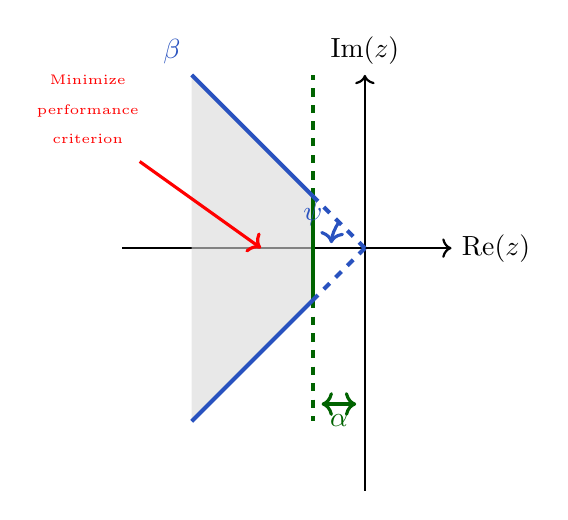
\begin{tikzpicture}[scale=2.2]
    \def\xmin{-1.4cm} \def\xmax{0.5cm}
    \def\ymin{-1.4cm} \def\ymax{1cm}

    \draw [thick,->] (\xmin,0) -- (\xmax,0) node [anchor = west]{$\operatorname{Re}(z)$};
    \draw [thick,->] (0,\ymin) -- (0,\ymax) node [anchor = south]{$\operatorname{Im}(z)$};
    \begin{scope}
      \clip (-1cm,-1cm) rectangle (-0.3cm,1cm);
      \fill[gray!30,opacity=0.6] (-0.3cm,0.3cm) -- (-0.3cm,-0.3cm) -- (-1cm,-1cm) -- (-1cm,1cm) -- cycle;
    \end{scope}
    \draw [darkGreen,line width= 0.5mm] (-0.3cm,-0.3cm) -- (-0.3cm,0.3cm);
    \draw [darkGreen,line width= 0.5mm,dashed] (-0.3cm,0.3cm) -- (-0.3cm,1cm);
    \draw [darkGreen,line width= 0.5mm,dashed] (-0.3cm,-0.3cm) -- (-0.3cm,-1cm);
    \draw [darkBlue,line width= 0.5mm, dashed] (0cm,0cm) -- (-0.3cm,0.3cm);
    \draw [darkBlue,line width= 0.5mm] (-0.3cm,0.3cm) -- (-1cm,1cm);
    \draw [darkBlue,line width= 0.5mm, dashed] (-1cm,1cm) -- (-1cm,1cm) node [pos=1,above left] {$\beta$};
    \draw [darkBlue,line width= 0.5mm, dashed] (0cm,0cm) -- (-0.3cm,-0.3cm);
    \draw [darkBlue,line width= 0.5mm] (-0.3cm,-0.3cm) -- (-1cm,-1cm);
    \draw[->,darkBlue,line width=0.4mm] (-0.15,0.15) arc[start angle=145, end angle=175, radius=0.25cm];
    \node[text=darkBlue] at (-0.3,0.2) {$\psi$};
    \draw[<->,darkGreen,line width=0.4mm] (-0.05,-0.9cm) -- (-0.25cm,-0.9cm) node[midway, below, text=darkGreen] {$\alpha$};
    % Arrow pointing to the gray region from the left
    \draw [->,red,line width=0.4mm] (-1.3cm,0.5cm) -- (-0.6cm,0cm);
    \node[text=red,align=center] at (-1.6cm,0.8cm) {\tiny Minimize\\[-0.05cm]\tiny performance\\[-0.05cm]\tiny criterion};
        \end{tikzpicture}
    \end{figure}
    %\end{column}

    % \begin{column}{0.45\textwidth}
    % \textbf{Design specifications:}

    % \vspace{0.3cm}
    % \textbf{Hard constraints:}

    % Pole placement in $\mathbb{D}_\alpha \cap \mathbb{D}_\beta$
    % \begin{itemize}
    %     \item \textcolor{darkGreen}{$\mathbb{D}_\alpha$:} minimum decay rate
    %     \item \textcolor{darkBlue}{$\mathbb{D}_\beta$:} damping ratio
    % \end{itemize}

    % \vspace{0.4cm}
    % \textbf{Soft constraint:}

    % Minimize $\|H_{wz}\|_{\mathcal{H}_2}^2$ performance
    % \end{column}
    % \end{columns}

     \vspace{0.4cm}
    \begin{center}
    \textbf{This is formulated as a convex optimization problem involving LMIs.}
    \end{center}
\end{frame}

\begin{frame}{Linear parameter varying control}{Proposed implementation: Constrained $\mathcal{H}_2$ LPV control}
    \textbf{Proposed approach:} LPV controller with "frozen" pole placement and $\mathcal{H}_2$ performance optimization.

       \begin{figure}
\begin{psfrags}
\def\textsize{.7}

\psfrag{Vr}[c][c][\textsize]{\color{blue4}$\rho^\#$}
\psfrag{thm}[c][c][\textsize]{\color{blue4}$\theta$}
\psfrag{wm}[c][c][\textsize]{\color{green4}$\omega$}
\psfrag{iabc}[c][c][\textsize]{\color{blue4}$i_{abc}$}
\psfrag{idq}[c][c][\textsize]{\color{blue4}$i_{dq}$}
\psfrag{vabcr}[c][c][\textsize]{\color{blue4}$v_{abc}^\#$}
\psfrag{vdq2}[c][c][\textsize]{\color{blue4}$v_{dq}^\#$}
\psfrag{dq}[c][c][.5]{\color{blue4}${dq}$}
\psfrag{abc}[c][c][.5]{\color{blue4}${abc}\quad$}
\psfrag{S}[c][c][\textsize]{\color{green4}$S_{abc}$}
\psfrag{ParkInv}[c][c][.5]{}
\psfrag{Park}[c][c][.5]{}
\psfrag{ref}[c][c][\textsize]{\color{cyan4}$\omega^\#$}

\psfrag{MLI}[c][c][.4]{\color{blue4}Modulation}
\psfrag{Onduleur}[c][c][\textsize]{\color{red4}Inverter}
\psfrag{PMSM}[c][c][\textsize]{\color{red4}PMSM}

\psfrag{V}[c][c][\textsize]{\color{red4}$v_{abc}$}
\psfrag{th}[c][c][\textsize]{\color{red4}$\theta$}
\psfrag{w}[c][c][\textsize]{\color{red4}$\omega$}
\newcommand{\sat}{\mathrm{sat}}

\psfrag{Dynamique}[c][c][\textsize]{\color{green4}Dynamic}
\psfrag{Asservissement}[c][c][\textsize]{\color{blue4}control}
\psfrag{Elec}[c][c][\textsize]{\color{blue4}Electrical}
\psfrag{Dynamique2}[c][c][\textsize]{\color{blue4}Dynamic}
\psfrag{Asservissement2}[c][c][\textsize]{\color{green4}control}
\psfrag{Meca}[c][c][\textsize]{\color{green4}Mechanical}
\psfrag{CapW}[c][c][\textsize]{\color{green2}Mechanical}

\psfrag{Idqr2}[c][c][\textsize]{\color{green4}{$i_{dq}^\#$}}
\psfrag{Idqr}[c][c][\textsize]{\color{green4}${i_{dq}^\#}$}
\psfrag{vdqr}[c][c][\textsize]{\color{blue4}$\sat({v_{dq}^\#})$}
\psfrag{+r}[c][c][\textsize]{\color{red4}$+$}
\psfrag{-r}[c][c][\textsize]{\color{red4}$-$}
\psfrag{+v}[c][c][\textsize]{\color{blue4}$+$}
\psfrag{-v}[c][c][\textsize]{\color{blue4}$-$}
\psfrag{+b}[c][c][\textsize]{\color{green4}$+$}
\psfrag{-b}[c][c][\textsize]{\color{green4}$-$}
\psfrag{ref1}[c][c][\textsize]{\color{blue4}$\frac{1}{s}$}
\psfrag{ref2}[c][c][\textsize]{\color{blue4}$K_i$}
\psfrag{ref3}[c][c][\textsize]{\color{blue4}$K_p$}
\psfrag{eq}[c][c][\textsize]{\color{blue4}$K_{dq}$}
\psfrag{x}[c][c][\textsize]{\color{blue4}$\times$}
\psfrag{vrep}[c][c][\textsize]{\color{blue4}$\varepsilon_{dq}$}
\psfrag{vdq}[c][c][\textsize]{\color{blue4}$v_{dq}$}

\psfrag{TSM}[l][c][.7]{\color{green4}$F_{s,m}= 1$kHz}
\psfrag{TSE}[l][c][.7]{\color{blue4}$F_{s,e}= 20$kHz}

\psfrag{Embedded}[l][c][1]{\color{red}Embedded code}

\includegraphics[width = \textwidth]{pictures/ControlFOCLPV.eps}
\end{psfrags}
\end{figure}
\end{frame}


\begin{frame}{Linear parameter varying control}{Classical implementation: PI + Feedback linearization}
    \textbf{Classical approach:} PI controller with feedback linearization to cancel nonlinearities.

       \begin{figure}
\begin{psfrags}
\def\textsize{.7}

\psfrag{Vr}[c][c][\textsize]{\color{blue4}$\rho^\#$}
\psfrag{thm}[c][c][\textsize]{\color{blue4}$\theta$}
\psfrag{wm}[c][c][\textsize]{\color{green4}$\omega$}
\psfrag{iabc}[c][c][\textsize]{\color{blue4}$i_{abc}$}
\psfrag{idq}[c][c][\textsize]{\color{blue4}$i_{dq}$}
\psfrag{vabcr}[c][c][\textsize]{\color{blue4}$v_{abc}^\#$}
\psfrag{vdq2}[c][c][\textsize]{\color{blue4}$v_{dq}^\#$}
\psfrag{dq}[c][c][.5]{\color{blue4}${dq}$}
\psfrag{abc}[c][c][.5]{\color{blue4}${abc}\quad$}
\psfrag{S}[c][c][\textsize]{\color{green4}$S_{abc}$}
\psfrag{ParkInv}[c][c][.5]{}
\psfrag{Park}[c][c][.5]{}
\psfrag{ref}[c][c][\textsize]{\color{cyan4}$\omega^\#$}

\psfrag{MLI}[c][c][.4]{\color{blue4}Modulation}
\psfrag{Onduleur}[c][c][\textsize]{\color{red4}Inverter}
\psfrag{PMSM}[c][c][\textsize]{\color{red4}PMSM}

\psfrag{V}[c][c][\textsize]{\color{red4}$v_{abc}$}
\psfrag{th}[c][c][\textsize]{\color{red4}$\theta$}
\psfrag{w}[c][c][\textsize]{\color{red4}$\omega$}
\newcommand{\sat}{\mathrm{sat}}

\psfrag{Dynamique}[c][c][\textsize]{\color{green4}Dynamic}
\psfrag{Asservissement}[c][c][\textsize]{\color{blue4}control}
\psfrag{Elec}[c][c][\textsize]{\color{blue4}Electrical}
\psfrag{Dynamique2}[c][c][\textsize]{\color{blue4}Dynamic}
\psfrag{Asservissement2}[c][c][\textsize]{\color{green4}control}
\psfrag{Meca}[c][c][\textsize]{\color{green4}Mechanical}
\psfrag{CapW}[c][c][\textsize]{\color{green2}Mechanical}

\psfrag{Idqr2}[c][c][\textsize]{\color{green4}{$i_{dq}^\#$}}
\psfrag{Idqr}[c][c][\textsize]{\color{green4}${i_{dq}^\#}$}
\psfrag{vdqr}[c][c][\textsize]{\color{blue4}$\sat({v_{dq}^\#})$}
\psfrag{+r}[c][c][\textsize]{\color{red4}$+$}
\psfrag{-r}[c][c][\textsize]{\color{red4}$-$}
\psfrag{+v}[c][c][\textsize]{\color{blue4}$+$}
\psfrag{-v}[c][c][\textsize]{\color{blue4}$-$}
\psfrag{+b}[c][c][\textsize]{\color{green4}$+$}
\psfrag{-b}[c][c][\textsize]{\color{green4}$-$}
\psfrag{ref1}[c][c][\textsize]{\color{blue4}$\frac{1}{s}$}
\psfrag{ref2}[c][c][\textsize]{\color{blue4}$K_i$}
\psfrag{ref3}[c][c][\textsize]{\color{blue4}$K_p$}
\psfrag{eq}[c][c][\textsize]{\color{blue4}$pL_{dq}\mathcal{J}$}
\psfrag{x}[c][c][\textsize]{\color{blue4}$\times$}
\psfrag{vrep}[c][c][\textsize]{\color{blue4}$\varepsilon_{dq}$}
\psfrag{vdq}[c][c][\textsize]{\color{blue4}$v_{dq}$}

\psfrag{TSM}[l][c][.7]{\color{green4}$F_{s,m}= 1$kHz}
\psfrag{TSE}[l][c][.7]{\color{blue4}$F_{s,e}= 20$kHz}

\psfrag{Embedded}[l][c][1]{\color{red}Embedded code}

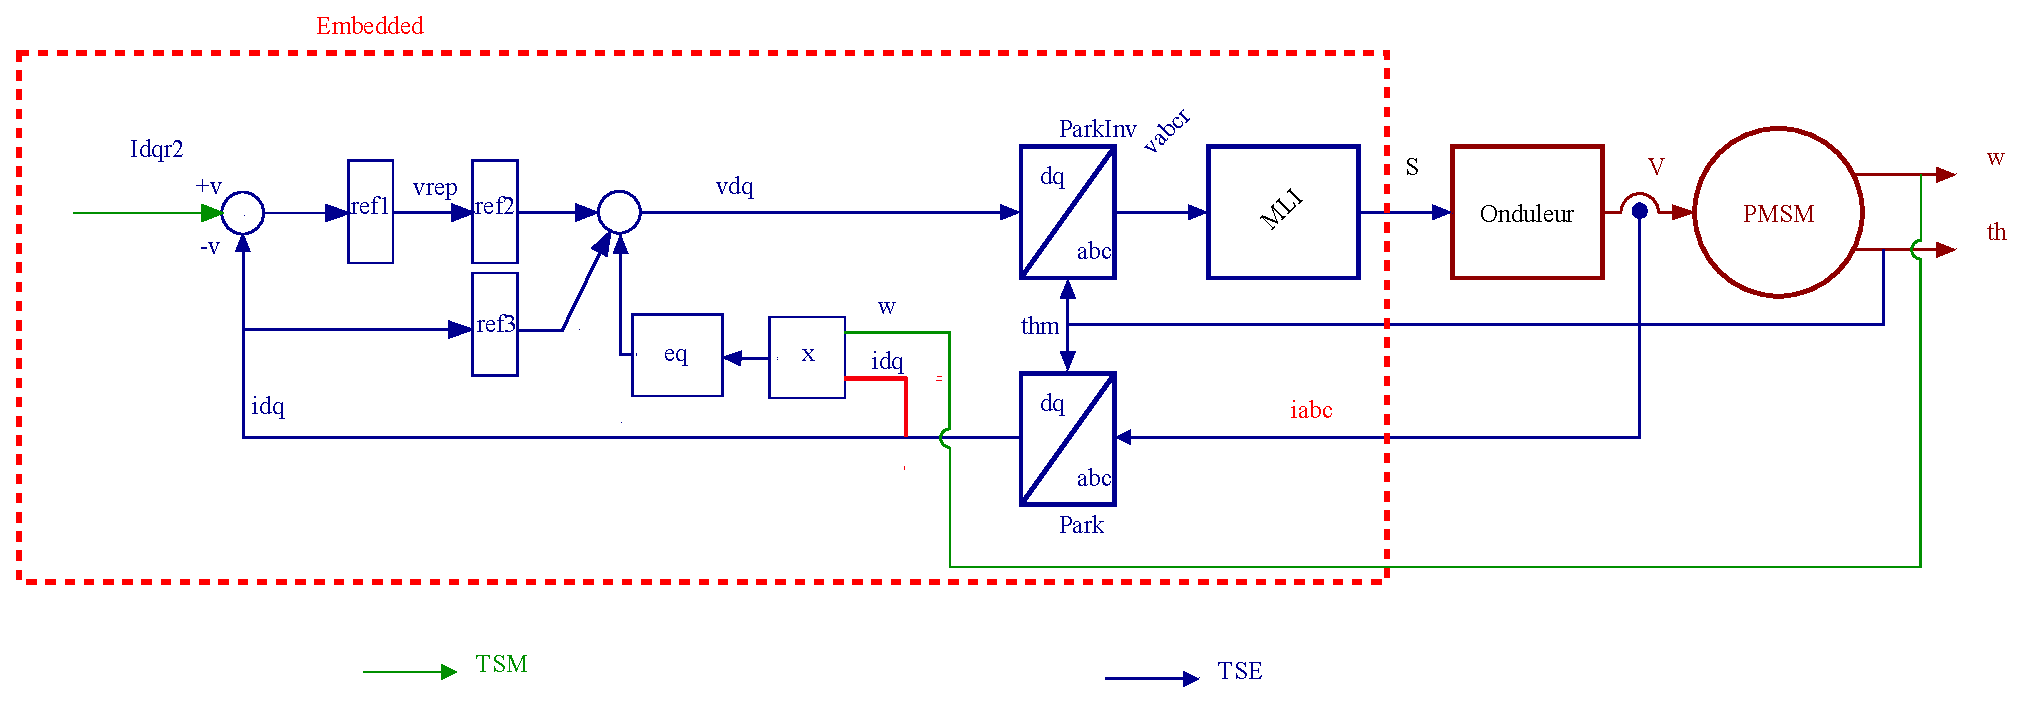
\includegraphics[width = \textwidth]{pictures/ControlFOCLPV_PI.eps}
\end{psfrags}
\end{figure}
\end{frame}


\begin{frame}{Linear parameter varying control}{Linearization-free approach}
    \textbf{Proposed approach:} Linearization-free control for PMSM through LMI-based synthesis.

    \vspace{0.3cm}
    \begin{columns}
        \begin{column}{0.5\textwidth}
        \textbf{PI + Feedback linearization}
           \begin{equation*}
               \begin{cases}
                    v_d = u_d -pL_q\omega i_q\\
                    v_q = u_q +pL_d\omega i_d
                \end{cases}
            \end{equation*}
            \vspace{0.2cm}
       \begin{itemize}
            \item[$-$] Direct current injection
            \item[$-$] High sensitivity to noise
            \item[$-$] No formal guarantees
        \end{itemize}
        \end{column}
        \begin{column}{0.5\textwidth}
            \textbf{Constrained-$\mathcal{H}_2$ LPV}
            \begin{equation*}
               \begin{cases}
                    v_d = u_d -K_d\omega \varepsilon_{i_q}\\
                    v_q = u_q +K_q\omega \varepsilon_{i_d}
                \end{cases}
            \end{equation*}
                    \vspace{0.2cm}
        \begin{itemize}
            \item[$+$] Reduced noise sensitivity
            \item[$+$] Stability via Lyapunov function
            \item[$+$] Performance guarantees
        \end{itemize}

        \end{column}
    \end{columns}
    \vspace{0.4cm}
    \begin{center}
    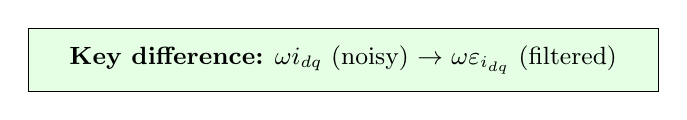
\begin{tikzpicture}
        \node[draw, rectangle, fill=green!10, minimum width=8cm, minimum height=0.8cm] {
            \begin{minipage}{7.5cm}
                \centering
                \small
                \textbf{Key difference:} $\omega i_{dq}$ (noisy) $\rightarrow$ $\omega \varepsilon_{i_{dq}}$ (filtered)
            \end{minipage}
        };
    \end{tikzpicture}
    \end{center}

\end{frame}


% \begin{frame}{LPV control}{Motivation}
%     \begin{figure}[H]
%     \centering
%     \includegraphics[trim=10cm 0.5cm 1cm 0.8cm, clip, width=0.85\textwidth]{pictures/LPV/control_law_corrected.eps}
%     \caption{Experiment validation for $\alpha = 49.98$}
%     \label{fig:alpha50}
%     \end{figure}
% \end{frame}

% \begin{frame}{LPV control: Motivation}
%     \textbf{Challenge with classical PI + feedback linearization:}

%     \vspace{0.3cm}
%     Classical approach is field-oriented control:
%      \begin{equation*}
%         v_{dq} = u_{dq} + pL_{dq}\omega \mathcal{J}i_{dq}
%     \end{equation*}

%     \vspace{0.2cm}
%     \begin{itemize}
%         \item[$-$] Injects current measurements directly into voltages
%         \item[$-$] Amplifies measurement noise, especially at high speeds
%         \item[$-$] No formal stability guarantee for time-varying speeds
%     \end{itemize}

%     \vspace{0.4cm}
%     \textbf{Goal:} Design a control that
%     \begin{itemize}
%         \item[$\checkmark$] Reduces noise sensitivity
%         \item[$\checkmark$] Guarantees performance for time-varying $\omega$
%         \item[$\checkmark$] Maintains intuitive tuning
%     \end{itemize}
% \end{frame}

% \begin{frame}{LPV systems framework}
%     \textbf{LPV state-space representation:}
%     \begin{align*}
%         \dot{x}(t) &= A(\rho(t))x(t) + B(\rho(t))u(t)\\
%         y(t) &= C(\rho(t))x(t) + D(\rho(t))u(t)
%     \end{align*}

%     where $\rho(t) \in \mathcal{R}^p$ is the scheduling parameter (measurable in real-time)

%     \vspace{0.3cm}
%     \textbf{Parameter-dependent controller:}
%     \begin{equation*}
%         u(t) = K(\rho(t))x(t)
%     \end{equation*}

%     \vspace{0.3cm}
%     \textbf{Key idea:} Use polytopic formulation
%     \begin{itemize}
%         \item Express system matrices as convex combinations at vertices
%         \item Check LMIs only at vertices (computationally tractable)
%         \item Use single quadratic Lyapunov function: $V(x) = x^\top P x$
%     \end{itemize}
% \end{frame}

% \begin{frame}{LPV model for IPMSM}
%     \textbf{Electrical dynamics with integral action:}
%     \begin{align*}
%         \dot{x} &= A(\omega)x + Bu + B_w w\\
%         z &= C_z x + D_z u
%     \end{align*}

%     where $x = [i_d,\, i_q,\, \varepsilon_{i_d},\, \varepsilon_{i_q}]^\top$

%     \vspace{0.3cm}
%     \textbf{Parameter-dependent matrix:}
%     \begin{equation*}
%         A(\omega) = A_c + A_l \omega
%     \end{equation*}

%     \vspace{0.2cm}
%     \textbf{Scheduling parameter:} $\omega \in \mathbf{\Omega} = [\omega_{min}, \omega_{max}]$

%     \vspace{0.3cm}
%     \textbf{Controller structure:}
%     \begin{equation*}
%         u = K(\omega)x = K_{pi}x + K_f \omega x
%     \end{equation*}
% \end{frame}

% \begin{frame}{Polytopic LPV formulation}
%     \textbf{Two vertices for speed range:} $\theta_1 = \omega_{min}$, $\theta_2 = \omega_{max}$

%     \vspace{0.3cm}
%     \textbf{Polytopic decomposition:}
%     \begin{equation*}
%         \omega = \sum_{i=1}^{2} \lambda_i \theta_i, \quad
%         A(\omega) = \sum_{i=1}^{2} \lambda_i A_i, \quad
%         K(\omega) = \sum_{i=1}^{2} \lambda_i K_i
%     \end{equation*}

%     with $\lambda_i \geq 0$ and $\lambda_1 + \lambda_2 = 1$

%     \vspace{0.3cm}
%     \textbf{Vertex gains:}
%     \begin{align*}
%         K_1 &= K_{pi} + K_f \omega_{min}\\
%         K_2 &= K_{pi} + K_f \omega_{max}
%     \end{align*}

%     \vspace{0.3cm}
%     $\Rightarrow$ \textbf{Finite LMI problem:} Check conditions only at $\omega_{min}$ and $\omega_{max}$
% \end{frame}

% \begin{frame}{Constrained-$\mathcal{H}_2$ LPV synthesis}
%     \textbf{Optimization problem at each vertex $i \in \{1,2\}$:}

%     \vspace{0.2cm}
%     \small
%     \begin{align*}
%         \min_{X,Y_i,W,\gamma} \quad & \gamma\\
%         \text{s.t.} \quad & \langle A_iX + BY_i \rangle_S + 2\alpha X \prec 0 \quad \text{(decay rate)}\\
%         & \begin{bmatrix}
%             \beta \langle A_iX + BY_i \rangle_S & (*)^\top\\
%             (A_iX + BY_i)^\top - (A_iX + BY_i) & \beta \langle A_iX + BY_i \rangle_S
%         \end{bmatrix} \prec 0\\
%         & \text{(damping)}\\
%         & \mathcal{H}_2 \text{ conditions} \quad \text{(noise minimization)}
%     \end{align*}

%     \normalsize
%     \vspace{0.2cm}
%     \textbf{Result:} Controller $K_i = Y_i X^{-1}$ guarantees:
%     \begin{itemize}
%         \item Performance in $\mathcal{D}_\alpha \cap \mathcal{D}_\beta$ for all $\omega \in \mathbf{\Omega}$
%         \item Minimized noise sensitivity
%     \end{itemize}
% \end{frame}

% \begin{frame}{Control structures comparison}
%     \begin{columns}[t]
%     \begin{column}{0.5\textwidth}
%         \textbf{PI + feedback linearization:}
%         \begin{equation*}
%             v_{dq} = u_{dq} + pL_{dq}\omega \mathcal{J}i_{dq}
%         \end{equation*}

%         \vspace{0.2cm}
%         \begin{itemize}
%             \item[$-$] Direct current injection
%             \item[$-$] High noise at high $\omega$
%             \item[$+$] Simple to implement
%         \end{itemize}
%     \end{column}

%     \begin{column}{0.5\textwidth}
%         \textbf{Constrained-$\mathcal{H}_2$ LPV:}
%         \begin{equation*}
%             v_{dq} = u_{dq} + K_{dq}\mathcal{J}\omega \varepsilon_{i_{dq}}
%         \end{equation*}

%         \vspace{0.2cm}
%         \begin{itemize}
%             \item[$+$] Uses integral (low-pass filter)
%             \item[$+$] Reduced noise sensitivity
%             \item[$+$] Formal stability guarantee
%         \end{itemize}
%     \end{column}
%     \end{columns}

%     \vspace{0.4cm}
%     \begin{center}
%     \begin{tikzpicture}
%         \node[draw, rectangle, fill=green!10, minimum width=8cm, minimum height=0.8cm] {
%             \begin{minipage}{7.5cm}
%                 \centering
%                 \small
%                 \textbf{Key difference:} $\omega i_{dq}$ (noisy) $\rightarrow$ $\omega \varepsilon_{i_{dq}}$ (filtered)
%             \end{minipage}
%         };
%     \end{tikzpicture}
%     \end{center}
% \end{frame}
% \begin{frame}{Linear parameter varying control}{Frozen parameter pole analysis}
%         \textbf{How do poles move with varying speed?}
%     \begin{columns}[]
%     \begin{column}{0.5\textwidth}
%     \textbf{PI control}
%         \only<1>{\includegraphics[width=0.9\columnwidth]{LPV_vs_PI/PI_0.eps}}
%         \only<2>{\includegraphics[width=0.9\columnwidth]{LPV_vs_PI/PI_200.eps}}
%         \only<3>{\includegraphics[width=0.9\columnwidth]{LPV_vs_PI/PI_400.eps}}
%         \only<4>{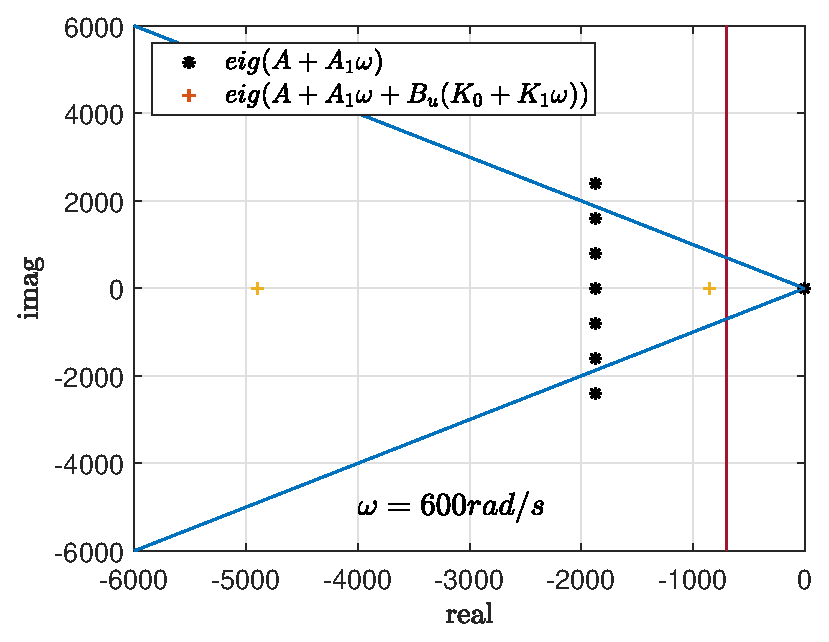
\includegraphics[width=0.9\columnwidth]{LPV_vs_PI/PI_600.eps}}
%         \only<5>{\includegraphics[width=0.9\columnwidth]{LPV_vs_PI/PI_800.eps}}
%     \small{\begin{equation*}
%                 \begin{cases}
%                 v_d = [K_{11}i_d +K_{13}\varepsilon_{i_{d}}]-\textcolor{red}{pL}\omega i_q\\
%                 v_q = [K_{22}i_q +K_{44}\varepsilon_{i_{q}}]+\textcolor{red}{pL} \omega i_d
%                 \end{cases}
%             \end{equation*}
%         }
%     \end{column}
%     \begin{column}{0.5\textwidth}

%     \textbf{Constrained LPV $\mathcal{H}_2$}

%         \only<1>{\includegraphics[width=0.9\columnwidth]{LPV_vs_PI/LPV_0.eps}}
%         \only<2>{\includegraphics[width=0.9\columnwidth]{LPV_vs_PI/LPV_200.eps}}
%         \only<3>{\includegraphics[width=0.9\columnwidth]{LPV_vs_PI/LPV_400.eps}}
%         \only<4>{\includegraphics[width=0.9\columnwidth]{LPV_vs_PI/LPV_600.eps}}
%         \only<5>{\includegraphics[width=0.9\columnwidth]{LPV_vs_PI/LPV_800.eps}}
%         \small{\begin{equation*}
%                 \begin{cases}
%                 v_d = [K_{11}i_d +K_{13}\varepsilon_{i_{d}}]-\textcolor{red}{K_d} \omega \colorbox{SpringGreen}{$\varepsilon_{i_{d}}$}\\
%                 v_q = [K_{22}i_q +K_{44} \varepsilon_{i_{q}}]+\textcolor{red}{K_q} \omega \colorbox{SpringGreen}{$\varepsilon_{i_{q}}$}
%                 \end{cases}
%         \end{equation*}
%        % $\:\varepsilon_{i_{d}=} \int_0^t (i_d - i_{d}^\#) dt $, $\varepsilon_{i_{q}=} \int_0^t (i_q - i_{q}^\#) dt $
%         }
%     \end{column}
%     \end{columns}
% \end{frame}

\begin{frame}{Linear parameter varying control}{Experimental validation}
\begin{columns}
    \begin{column}{0.5\textwidth}
        \begin{figure}[H]
        \centering
        \includegraphics[trim={0cm 5cm 2cm 0cm},clip,width=1\columnwidth]{pictures/Banc_IPMSM.eps}
        \caption{PMSM test bench.}
        \label{fig:bancIPMSM_sec3}
    \end{figure}    
    \end{column}
    \begin{column}{0.5\textwidth}
        \vspace{-1.5cm}
                     \begin{figure}
             \centering
         \includegraphics[trim={0.8cm 0.7cm 1.5cm 0.2cm},clip,width=1\columnwidth]{pictures/current_step.eps}
            \end{figure}
    \end{column}
\end{columns}
    

 %   \vspace{0.3cm}

   % \begin{columns}
     % \begin{column}{0.5\textwidth}

        % \end{column}
      %  \begin{column}{0.5\textwidth}
        % % %   \only<1>{  \begin{figure}
        % % %     \centering
        % % %     \includegraphics[trim={0.4cm 8.9cm 1.4cm 10.2cm},clip,width=0.7\textwidth]{pictures/current_step.eps}
        % % %     \end{figure} }
            
        % % %     \only<2>{  
        % % %     \begin{figure}
        % % %         \centering
        % % %         \includegraphics[trim={0.4cm 1.4cm 1.4cm 11.5cm},clip,width=0.7\textwidth]{pictures/current_step.eps}
        % % %     \end{figure}}
            %trim={<left> <bottom> <right> <top>}
       % \end{column}
  %  \end{columns}
\end{frame}

% \begin{frame}{Frozen parameter pole analysis}
%     \textbf{How do poles move with varying speed?}

%     \vspace{0.3cm}
%     \begin{columns}[t]
%     \begin{column}{0.5\textwidth}
%         \centering
%         \textbf{PI feedback linearization}

%         \vspace{0.2cm}
%         \begin{itemize}
%             \item Cancels speed-dependent terms
%             \item Fixed pole locations
%             \item Independent of $\omega$
%         \end{itemize}

%         \vspace{0.2cm}
%         \small
%         \textcolor{gray}{(See figure in thesis)}
%     \end{column}

%     \begin{column}{0.5\textwidth}
%         \centering
%         \textbf{Constrained-$\mathcal{H}_2$ LPV}

%         \vspace{0.2cm}
%         \begin{itemize}
%             \item Adapts to speed variation
%             \item Poles move within $\mathcal{D}_\alpha \cap \mathcal{D}_\beta$
%             \item Preserves natural dynamics
%         \end{itemize}

%         \vspace{0.2cm}
%         \small
%         \textcolor{gray}{(See figure in thesis)}
%     \end{column}
%     \end{columns}

%     \vspace{0.4cm}
%     \textbf{Note:} Analysis at "frozen" speeds gives intuition, but LPV guarantees performance for time-varying $\omega$
% \end{frame}

% \begin{frame}{Sensitivity function analysis}
%     \textbf{Transfer function from sensor noise $w_d$ to:}

%     \vspace{0.3cm}
%     \begin{itemize}
%         \item \textbf{Control input $v_q$:}
%         \begin{itemize}
%             \item Constrained-$\mathcal{H}_2$ shows better roll-off at high frequencies
%             \item Reduced noise amplification compared to PI
%         \end{itemize}

%         \vspace{0.2cm}
%         \item \textbf{Performance output $i_q$:}
%         \begin{itemize}
%             \item Better decoupling between d-q axes
%             \item Lower cross-axis sensitivity
%         \end{itemize}
%     \end{itemize}

%     \vspace{0.3cm}
%     \textbf{Why better high-frequency attenuation?}
%     \begin{itemize}
%         \item $\mathcal{H}_2$ optimization minimizes energy across spectrum
%         \item Integral action provides natural low-pass filtering
%     \end{itemize}

%     \vspace{0.2cm}
%     $\Rightarrow$ \textbf{More robust and noise-resilient control at no added computational cost}
% \end{frame}

% \begin{frame}{Experimental validation: Setup}
%     \textbf{Test bench:} IPMSM with dSpace MicroLabBox

%     \vspace{0.3cm}
%     \textbf{Two experiments:}

%     \vspace{0.2cm}
%     \textbf{1) Torque step at constant speed (3000 rpm):}
%     \begin{itemize}
%         \item Evaluate transient behavior
%         \item Both controls tuned for same dynamics
%     \end{itemize}

%     \vspace{0.3cm}
%     \textbf{2) Speed ramp (500 to 4000 rpm):}
%     \begin{itemize}
%         \item Evaluate steady-state at various speeds
%         \item Covers MTPA and field-weakening regions
%     \end{itemize}

%     \vspace{0.3cm}
%     \textbf{Measured signals:} $\omega$, $v_d$, $v_q$, $i_d$, $i_q$

%     \vspace{0.2cm}
%     \textbf{Comparison:} PI + feedback linearization vs. Constrained-$\mathcal{H}_2$ LPV
% \end{frame}

% \begin{frame}{Experimental results: Key findings}
%     \textbf{Voltage quality:}
%     \begin{itemize}
%         \item[$\checkmark$] \textbf{Smoother voltages $v_{dq}$} with constrained-$\mathcal{H}_2$
%         \item[$\checkmark$] Reduced high-frequency noise
%         \item[$\checkmark$] Especially visible on $v_d$ (higher $i_q$ amplitude)
%     \end{itemize}

%     \vspace{0.3cm}
%     \textbf{Current dynamics:}
%     \begin{itemize}
%         \item[$\checkmark$] \textbf{Identical $i_d$ and $i_q$ dynamics} for both methods
%         \item[$\checkmark$] Same transient response (as designed)
%         \item Both affected by same sensor noise (-20 dB for PI, -50 dB for $\mathcal{H}_2$)
%     \end{itemize}

%     \vspace{0.3cm}
%     \begin{center}
%     \begin{tikzpicture}
%         \node[draw, rectangle, fill=blue!10, minimum width=8cm, minimum height=0.8cm] {
%             \begin{minipage}{7.5cm}
%                 \centering
%                 \textbf{Same dynamics + Less noisy inputs = Better performance}
%             \end{minipage}
%         };
%     \end{tikzpicture}
%     \end{center}

%     \vspace{0.2cm}
%     \small
%     \textcolor{gray}{See detailed experimental plots in thesis: Figures 4.11 and 4.12}
% \end{frame}

\begin{frame}{Linear parameter varying control}{LPV control: Summary}
    \textbf{Contributions:}
    \begin{itemize}
        \item \textbf{Linearization-free control:} No exact cancellation needed
        \item \textbf{Performance guarantees:} Lyapunov certificate for time-varying $\omega$
        \item \textbf{Noise reduction:} filtering effect due to the  $\mathcal{H}_2$ optimization 
        \item \textbf{Experimental validation:} Confirmed on PMSM test bench
    \end{itemize}

    % \vspace{0.3cm}
    % \textbf{Advantages over classical PI:}
    % \begin{itemize}
    %     \item[$+$] Same computational cost (no additional online computation)
    %     \item[$+$] Maintains classical nested structure (easy integration)
    %     \item[$+$] Intuitive tuning via $\alpha$, $\beta$ parameters
    %     \item[$+$] Better noise rejection
    % \end{itemize}

    \vspace{0.3cm}
    \textbf{Other work:}
    \begin{itemize}
        \item Robustness to parametric uncertainty $\rightarrow$  norm-bounded parametric  uncertainty
    \end{itemize}
\end{frame}

% \begin{frame}{Polynomial transformation for voltage constraint}
%     The polynomial form for a given  IPMSM with parameters $R$ $L_d$, $L_q$, $\phi_f$, $p$:
%     \begin{equation*}
%         h(i_d, \tau, \omega) = a_4(\tau,\omega) i_d^4 + a_3(\tau,\omega) i_d^3 + a_2(\tau,\omega) i_d^2 + a_1(\tau,\omega) i_d + a_0(\tau,\omega)
%     \end{equation*}
%     \pause
%     \vspace{0.3cm}
%     \textbf{Domain of interest:}
%     \begin{equation*}
%         \mathcal{S} = \{i_d, \omega, \tau \in \mathcal{R} \:|\: i_d \in [-i_{max},0], \: \omega \geqslant 0, \: \tau \geqslant 0\}
%     \end{equation*}
%     \pause
%     \textbf{Challenge:} Proving $ h(i_d, \tau, \omega) \geqslant 0$ over $\mathcal{S}$
% \end{frame}



% % \begin{frame}{Higher-order coefficients analysis}
% %     Recall the polynomial form:
% %     \begin{equation*}
% %         h(i_d,\omega,\tau) = a_4 i_d^4 + a_3 i_d^3 + a_2 i_d^2 + a_1 i_d + a_0
% %     \end{equation*}

% %     \pause
% %     \vspace{0.3cm}
% %     For the IPMSM parameters, we observe:
% %     \begin{eqnarray*}
% %         a_4 &\geqslant 0, \quad \forall \: \omega, \tau, i_d \in \mathcal{S} \\
% %         a_3 &\leqslant 0, \quad \forall \: \omega, \tau, i_d \in \mathcal{S}, \quad \text{since } (L_d-L_q) < 0 \\
% %         a_2 &\geqslant 0, \quad \forall \: \omega, \tau, i_d \in \mathcal{S}
% %     \end{eqnarray*}

% %     \pause
% %     \vspace{0.3cm}
% %     \textbf{Strategy:} Decompose the polynomial to verify non-negativity.
% % \end{frame}

% \begin{frame}{Polynomial decomposition: $h = h_1 + h_2$}
%     We decompose the polynomial $h(i_d,\omega,\tau)$ into two parts:
%     \begin{equation*}
%         h(i_d,\omega,\tau) = \underbrace{a_4 i_d^4 + a_3 i_d^3 + a_2 i_d^2}_{h_1(i_d,\omega,\tau)} + \underbrace{a_1 i_d + a_0}_{h_2(i_d,\omega,\tau)}
%     \end{equation*}

%     \pause
%     \vspace{0.4cm}
%     \textbf{Analysis of each part:}
%     \begin{itemize}
%         \item \textbf{$h_1$:} Higher-order terms ($i_d^4$, $i_d^3$, $i_d^2$)
%         \item \textbf{$h_2$:} Lower-order terms (linear and constant)
%     \end{itemize}
% \end{frame}

% \begin{frame}{Non-negativity of $h_1$: easily proven}
%     Recall the signs of coefficients:
%     \begin{eqnarray*}
%         a_4 &\geqslant 0, \quad \forall \: \omega, \tau, i_d \in \mathcal{S} \\
%         a_3 &\leqslant 0, \quad \forall \: \omega, \tau, i_d \in \mathcal{S} \\
%         a_2 &\geqslant 0, \quad \forall \: \omega, \tau, i_d \in \mathcal{S}
%     \end{eqnarray*}

%     \pause
%     \vspace{0.3cm}
%     The sum of these three terms is guaranteed to be non-negative:
%     \begin{equation*}
%         h_1(i_d,\omega,\tau) = a_4 i_d^4 + a_3 i_d^3 + a_2 i_d^2 \geqslant 0
%     \end{equation*}
%     \textcolor{green}{$\forall (i_d,\omega,\tau) \in \mathcal{S}$}

%     \pause
%     \vspace{0.3cm}
%     \textcolor{red}{\textbf{Remaining challenge:}} Prove non-negativity of $h_2(i_d,\omega,\tau) = a_1 i_d + a_0$
% \end{frame}

% \begin{frame}{Proving non-negativity of $h_2$ using Sum of Squares (SoS)}
%     \textbf{Challenge:} Analytically determining the signs of coefficients $a_1(\omega,\tau)$ and $a_0(\omega,\tau)$ over domain $\mathcal{S}$ is complex.

%     \pause
%     \vspace{0.3cm}
%     \textbf{Solution:} Use \textcolor{blue}{\textbf{Sum of Squares (SoS) programming}} for formal verification.

%     \pause
%     \vspace{0.3cm}
%     \textbf{What is SoS?}
%     \begin{itemize}
%         \item A technique for certifying polynomial non-negativity over semialgebraic sets
%         \item Represents a polynomial as: $p(x) = \sum_i q_i^2(x)$
%         \item Sum of squares $\Rightarrow$ \textcolor{green}{globally non-negative}
%         \item Provides \textcolor{green}{\textbf{formal guarantees}}
%         \item Can be solved via \textcolor{blue}{convex optimization (SDP)}
%     \end{itemize}
% \end{frame}

% \begin{frame}{SoS decomposition for $h_2$}
%     We construct a Positivstellensatz-type SoS decomposition:
%     \begin{equation*}
%         \begin{split}
%         h_2(i_d,\omega,\tau) = s_0(i_d,\omega,\tau) + s_1(i_d)(i_d+i_{max}) \\
%         + s_2(i_d)(-i_d) + s_3(\omega)\omega + s_4(\tau)\tau
%         \end{split}
%     \end{equation*}

%     \pause
%     \vspace{0.3cm}
%     where:
%     \begin{itemize}
%         \item Each $s_j$ is a \textcolor{blue}{\textbf{SoS polynomial}} (to be determined)
%         \item Terms $(i_d+i_{max}) \geqslant 0$, $(-i_d) \geqslant 0$, $\omega \geqslant 0$, $\tau \geqslant 0$ represent the non-negative constraints defining domain $\mathcal{S}$
%     \end{itemize}

%     \pause
%     \vspace{0.3cm}
%     \textcolor{green}{\textbf{If this decomposition exists:}} $h_2(i_d,\omega,\tau) \geqslant 0, \quad \forall (i_d,\omega,\tau) \in \mathcal{S}$
% \end{frame}

% \begin{frame}{Convexity conclusion}
%     \textbf{Summary of the proof:}
%     \pause
%     \vspace{0.2cm}
%     \textbf{Step 1:} Analytical proof of higher-order terms:
%     \begin{equation*}
%         h_1(i_d,\omega,\tau) = a_4 i_d^4 + a_3 i_d^3 + a_2 i_d^2 \geqslant 0, \quad \forall (i_d,\omega,\tau) \in \mathcal{S}
%     \end{equation*}
%     \pause
%     \textbf{Step 2:} Using SoS verification (YALMIP + MOSEK) for lower-order terms:
%     \begin{equation*}
%         h_2(i_d,\omega,\tau) = a_1 i_d + a_0 \geqslant 0, \quad \forall (i_d,\omega,\tau) \in \mathcal{S}
%     \end{equation*}
%     \pause
%     \textbf{Step 3:} Combining both results:
%     \begin{equation*}
%         h(i_d,\omega,\tau) = h_1 + h_2 \geqslant 0, \quad \forall (i_d,\omega,\tau) \in \mathcal{S}
%     \end{equation*}
%     \pause
%     \textbf{Step 4:} Since $h(i_d,\omega,\tau) = (K_1+K_2 i_d)^4 c_v''(i_d,\omega,\tau)$ and $(K_1+K_2 i_d)^4 > 0$:
%     \begin{equation*}
%         c_v''(i_d,\omega,\tau) \geqslant 0, \quad \forall (i_d,\omega,\tau) \in \mathcal{S}
%     \end{equation*}
%     \pause
%     \vspace{0.2cm}
%     \textcolor{green}{\textbf{Conclusion:}} The OTC formulation is \textcolor{green}{\textbf{convex}} over $\mathcal{S}$ for the IPMSM parameters!
% \end{frame}
%%%%%%%%%%%%%%%% Convex optimization : closed-loop  control
% \begin{frame}{Outline}
%             Implement \textcolor{Red}{advanced control laws synthesis} on \textcolor{ceruleanblue}{low-cost hardware} to drive \textcolor{Green}{real-world systems}.
%      \vspace{-0.5cm}
%      \begin{figure}
%         %\centering
%         \begin{tikzpicture}[scale= 0.8]
%         % Reserve space for all elements to prevent coordinate system shifts
%         \coordinate (origin) at (0,0);
%          % Green circle - appears from slide 4 onwards
%             \draw [gray, line width=0.8mm](0,-1.5) circle (2);
%             \node at (0,-2.5) {\textcolor{gray}{\shortstack{Control \\ Application}}};
%             \draw [red,line width=0.8mm] (-1.3,0) circle (2);% Red circle - persistent from slide 2 onwards
%             \node at (-1.8,1) {\textcolor{red}{\shortstack{Convex \\ Optimization}}};
%             \node at (-8.5,2) {\includegraphics[width=2.5cm]{pictures/Robust_control_law.eps}};
%             \node at (-5.5,2) {\includegraphics[width=2.5cm]{pictures/Robust_control_law.eps}};
%             \node at (-5.5,0) {\shortstack{Feedback \\ control}};
%             \node at (-8.5,0) {\shortstack{Trajectory \\ generation}};
%             \draw [red, line width=0.6mm, dashed, ->] (-2,2) to [bend right=15] (-4,2);
%             \draw [gray,line width=0.8mm] (1.3,0) circle (2);% Blue circle - appears from slide 3 onwards
%             \node at (1.7,1) {\textcolor{gray}{\shortstack{Embedded \\ systems}}};
%         % Invisible bounding box to maintain consistent tikzpicture size
%         \path[use as bounding box] (-10,-5) rectangle (10,3);
%         \end{tikzpicture}
%      \end{figure}
% \end{frame}

%%%%%%%%%%%%%%%% Convex optimization : closed-loop  control
% \begin{frame}{Outline}
%         Implement \textcolor{Red}{advanced control laws synthesis} on \textcolor{ceruleanblue}{low-cost hardware} to drive \textcolor{Green}{real-world systems}.
%      \vspace{-0.5cm}
%     \begin{figure}
%         \hspace{-2.5cm}\begin{tikzpicture}[scale= 0.8]
%         \coordinate (origin) at (0,0);
%             \draw [gray, line width=0.8mm](0,-1.5) circle (2);% Green circle - appears from slide 4 onwards
%             \node at (0,-2.5) {\textcolor{gray}{\shortstack{Control \\ Application}}};
%         \draw [gray,line width=0.8mm] (-1.3,0) circle (2);   % Red circle - persistent from slide 2 onwards
%         \node at (-1.8,1) {\textcolor{gray}{\shortstack{Convex \\ Optimization}}};
%         \draw [ceruleanblue,line width=0.8mm] (1.3,0) circle (2);% Blue circle - appears from slide 3 onwards
%         \node at (1.7,1) {\textcolor{ceruleanblue}{\shortstack{Embedded \\ systems}}};
%         \node at (5,1) {\includegraphics[width=2.5cm]{pictures/muC.eps}};
%             \node at (5,-1) {\shortstack{Microcontrollers \\ DSP}};
%             \draw [ceruleanblue, line width=0.6mm, dashed, ->] (2,2) to[bend left=15] (4.5,2);
%         \path[use as bounding box] (-10,-5) rectangle (10,3);% Invisible bounding box to maintain consistent tikzpicture size
%         \end{tikzpicture}
%      \end{figure}
% \end{frame}
% \begin{frame}{Dynamical model}
%     \vspace{-0.5cm}
% The nonlinear model of the system in the dq frame can  be represented as
%             \begin{eqnarray*}
%                \tikz[remember picture,overlay] {
%                      \draw[dashed,thick,rounded corners,blue] (-0.5,-1.3) rectangle (8,0.7);
%                     \node[right] at (8.1,-0.3) {\textcolor{blue}{Electrical dynamic}};

%                     \draw[dashed,thick,rounded corners,green!60!black] (8,-3.5) rectangle (-0.5,-1.8) ;
%                     \node[right] at (8.1,-2.65){\textcolor{green!60!black}{Mechanical dynamic}};

%                     \draw[dashed,thick,rounded corners,red!60!black] (8,-3.8) rectangle (-0.5,-4.6) ;
%                     \node[right] at (8.1,-4.15){\textcolor{red!60!black}{Current constraint}};

%                     \draw[dashed,thick,rounded corners, yellow!60!black] (8,-4.8) rectangle (-0.5,-5.6) ;
%                     \node[right] at (8.1,-5.15){\textcolor{yellow!60!black}{Voltage constraint}};

%                     \draw[dashed,thick,rounded corners, brown] (8,-5.8) rectangle (-0.5,-6.9) ;
%                     \node[right] at (8.1,-6.3){\textcolor{brown}{Reference trajectories}};
%                     }
%                      \frac{di_d}{dt} &=& \frac{1}{L_d}v_d - \frac{R}{L_d}i_d \textcolor{red}{+p\omega i_q}, \\
%                      \frac{di_q}{dt} &=& \frac{1}{L_q}v_q -\frac{R}{L_q}i_q \textcolor{red}{-p\omega i_d} -\frac{p \phi_f}{L_q}\omega, \\
%              \\
%              \\
%             \frac{d\omega}{dt} &=& \underbrace{\frac{3p\phi_f}{2J}i_q +  \textcolor{red}{\frac{3}{2J}p (L_d - L_q) i_d i_q }}_{\tau_{em}}  -\frac{f}{J}\omega \textcolor{violet}{-\tau_l}
%              \end{eqnarray*}
% subject to the following constraints
%              \begin{equation*}
%                 i_{dq}^\top i_{dq} - i_{max}^2 \leqslant 0
%                 \label{eq:idq_current_constraint}
%             \end{equation*}
%             \begin{equation*}
% 	            v_{dq}^\top v_{dq} - v_{max}^2 \leqslant 0.
%                 \label{eq:vdq_voltage_constraint}
%             \end{equation*}
%             \begin{equation*}
%                 \omega^\# , \quad \tau^\#_{em} = \frac{3p\phi_f}{2J}i_q +  \textcolor{red}{\frac{3}{2J}p (L_d - L_q) i_d i_q }
%             \end{equation*}
%  \end{frame}


% ========================================
% Section 4: Conclusion
% ========================================
\section{Conclusion}
\begin{frame}

    \centering
    Conclusions and Perspectives
    
\end{frame}
\begin{frame}{Conclusions Summary}
    \begin{columns}[T]
        \begin{column}{0.33\textwidth}
            \centering
            \textbf{\textcolor{blue}{Optimal Torque Control}}

            \vspace{0.3cm}
            \small
            \begin{itemize}
                \item Change of variable
                \item New formulation of OTC problem
                \item Convexity proof via Sum-of-Squares programming
                \item Interior-point solver for optimal torque trajectories
               % \item Experimental validation
            \end{itemize}
        \end{column}

        \begin{column}{0.33\textwidth}
            \centering
            \textbf{\textcolor{blue}{Embedded Synthesis}}

            \vspace{0.3cm}
            \small
            \begin{itemize}
                \item Pole-constrained $\mathcal{H}_2$ synthesis
                \item Embedded LMI solver (idle task)
                \item 0.3s computation time
               % \item Experimental validation
               % \item Guaranteed transient specifications
            \end{itemize}
        \end{column}

        \begin{column}{0.33\textwidth}
            \centering
            \textbf{\textcolor{blue}{LPV Control}}

            \vspace{0.3cm}
            \small
            \begin{itemize}
                \item Linearization-free control
                \item Lyapunov certificate for time-varying $\omega$ (LMI-based synthesis)
                \item Noise reduction at no additional embedded computational cost

            \end{itemize}
        \end{column}
    \end{columns}
          \begin{center}
    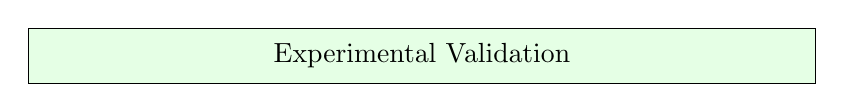
\begin{tikzpicture}
        \node[draw, rectangle, fill=green!10, minimum width=10cm, minimum height=0.7cm] {
            \begin{minipage}{9.5cm}
                \centering
               Experimental Validation 
            \end{minipage}
        };
    \end{tikzpicture}
    \end{center}
    \vspace{0.5cm}
    \centering
    \textbf{\textcolor{violet}{What is next ? }}
\end{frame}

\begin{frame}{Short-term perspectives}
    \begin{columns}[T]
        \begin{column}{0.33\textwidth}
            \centering
            \textbf{\textcolor{blue}{Optimal Torque Control}}

            \vspace{0.3cm}
            \small
            \begin{itemize}
                \item Extend the convex formulation to other types of machines
                \item Generic embedded solver for all synchronous machines
            \end{itemize}
        \end{column}

        \begin{column}{0.33\textwidth}
            \centering
            \textbf{\textcolor{blue}{Embedded Synthesis}}

            \vspace{0.3cm}
            \small
            \begin{itemize}
                \item Exploit the sparsity of the matrices
                \item Better tuning of the interior-point method (ADMM...)
                %\item
               % \item Guaranteed transient specifications
            \end{itemize}
        \end{column}

        \begin{column}{0.33\textwidth}
            \centering
            \textbf{\textcolor{blue}{LPV Control}}

            \vspace{0.3cm}
            \small
            \begin{itemize}
                \item Explore other nonlinear types of control (Sum-of-Squares)
                \item Include input and state saturations in the LMI synthesis
            \end{itemize}
        \end{column}
    \end{columns}
\end{frame}




% ========================================
% Section 5: Perspectives
% ========================================
\section{Perspectives}
\begin{frame}{Long-term perspectives}
     \begin{figure}
            \begin{center}
                \def\textsize{.8}
                \psfrag{Algo}[c][c][1]{\color{Blue4}Control}
                \psfrag{Control}[c][c][1]{\color{Blue4}Control}
                \psfrag{iabc}[c][c][\textsize]{\color{Blue4}$i_{abc}$}
                \psfrag{idq}[c][c][\textsize]{\color{Blue4}$i_{dq}$}
                
                \psfrag{Sys}[c][c][\textsize]{\color{Magenta4}System}
                \psfrag{identif}[c][c][\textsize]{\color{Magenta4} identification}
                \psfrag{vabcr}[c][c][\textsize]{\color{Blue4}$v_{abc}^\#$}
                \psfrag{vdqr}[c][c][\textsize]{\color{Blue4}$v_{dq}^\#$}
                \psfrag{dq}[c][c][.5]{\color{Blue4}${dq}$}
                \psfrag{abc}[c][c][.5]{\color{Blue4}${abc}\quad$}
                \psfrag{S}[c][c][\textsize]{\color{Blue4}$S_{abc}$}
                \psfrag{MLI}[c][c][\textsize]{\color{Blue4}Mod}
                \psfrag{ParkInv}[c][c][.5]{}
                \psfrag{Park}[c][c][.5]{}
                \psfrag{TS1}[l][c][.6]{\color{Blue4}Higher priority $\approx20$kHz}
                % Reference generation (cyan) - lower priority optimization
                \psfrag{Vr}[c][c][\textsize]{\color{Cyan4}$\rho^\#$}
                \psfrag{ref}[c][c][\textsize]{\color{Cyan4}$\omega^\#$}
                \psfrag{ref2}[c][c][\textsize]{\color{Cyan4}$i_d^\#$}
                \psfrag{ref3}[c][c][\textsize]{\color{Cyan4}$\omega^\#$}
                \psfrag{ref4}[c][c][\textsize]{\color{Cyan4}$i_q$}
                \psfrag{ref5}[c][c][\textsize]{\color{Magenta4} Specification}
                \psfrag{ref6}[c][c][\textsize]{\color{Magenta4} Model}
                \psfrag{Reference}[c][c][\textsize]{\color{Cyan4}Trajectory}
                \psfrag{calculation}[c][c][\textsize]{\color{Cyan4}generation}
                \psfrag{TS2}[l][c][.6]{\color{Cyan4}Lower priority $\approx1$kHz}
                % Embedded synthesis (magenta) - idle task
                \psfrag{Emb}[c][c][\textsize]{\color{Magenta4}Embedded}
                \psfrag{Synt}[c][c][\textsize]{\color{Magenta4}synthesis}
                \psfrag{K}[c][c][\textsize]{\color{Magenta4}K}
                \psfrag{TS3}[l][c][.6]{\color{Magenta4}Idle task}
                \psfrag{ref7}[l][c][.6]{\color{Magenta4}Data}
                % Physical system (red) - PMSM and measurements
                \psfrag{Onduleur}[c][c][\textsize]{\color{Red4}Invert}
                \psfrag{PMSM}[c][c][\textsize]{\color{Red4}PMSM}
                \psfrag{V}[c][c][\textsize]{\color{Red4}$v_{abc}$}
                \psfrag{th}[c][c][\textsize]{\color{Red4}$\theta$}
                \psfrag{w}[c][c][\textsize]{\color{Red4}$\omega$}
                \psfrag{thm}[c][c][\textsize]{\color{Red4}$\theta$}
                \psfrag{wm}[c][c][\textsize]{\color{Red4}$\omega$}
                \psfrag{Embedded}[l][c][.7]{\color{red}Embedded code}
                \includegraphics[width = .9\textwidth]{pictures/AdvancedControl_ident.eps}
            \end{center}
       % \label{fig:AdvencedControlForElectricalMotor}
        \end{figure}
        \vspace{+0.3cm}
        \centering
        \textbf{Vision:} Fully embedded, \textcolor{blue}{plug-and-play} control system integrating parameter estimation, control synthesis, and real-time optimization

\end{frame}
%\end{frame}

% \begin{frame}{Long-term Vision and Future Directions}

%     \vspace{0.3cm}

%             \centering
%             \textbf{\textcolor{blue}{Generalization}}

%             \vspace{0.2cm}
%             \small
%             \begin{itemize}
%                 \item Power electronic converters
%                 \item Energy generators (wind farms)
%                 \item Robotic actuators
%                 \item Autonomous systems requiring online adaptation
%                 \item Other types of machines (Poly-phase machines, Synchronous reluctance, induction...)
%             \end{itemize}

% \end{frame}

\section{Publications}
\begin{frame}{Publications}
    \footnotesize
    \vspace{-0.2cm}
    \begin{samepage}
            \begin{enumerate}[leftmargin=*, labelsep=0.3em, align=left, widest={[\textbf{S.1}]}, itemindent=0em, label={\textbf{[\arabic*]}]}, itemsep=0.3em]
            \item[\textbf{[C.1]}]  \textbf{A Karush-Kuhn-Tucker approach to field-weakening for Surface-Mounted Permanent Magnets Synchronous Motors}\\
            \mbox{\textbf{\textit{Hiba Houmsi}}}, \mbox{Federico Bribiesca-Argomedo}, \mbox{Paolo Massioni}, \mbox{Romain Delpoux}.\\
            \textit{IEEE International Conference on Control, Automation and Diagnosis (ICCAD), Rome, Italy, 2023}

            \item[\textbf{[C.2]}] \textbf{Embedded Controller Optimization for Efficient Electric Motor Drive} \\
            \mbox{\textbf{\textit{Hiba Houmsi}}}, \mbox{Paolo Massioni}, \mbox{Federico Bribiesca-Argomedo}, \mbox{Romain Delpoux}.\\
            \textit{IEEE Vehicle Power and Propulsion Conference (VPPC), Milan, Italy, 2023}

            \item[\textbf{[C.3]}] \textbf{Robust Pole-constrained $\mathcal{H}_2$ Controller for Permanent Magnet Synchronous Motors} \\
            \mbox{\textbf{\textit{Hiba Houmsi}}}, \mbox{Paolo Massioni}, \mbox{Federico Bribiesca-Argomedo}, \mbox{Romain Delpoux}.\\
            \textit{IEEE 23rd European control conference, Thessaloniki, Greece, 2025}

            \item[\textbf{[C.4]}] \textbf{Real-Time Interior-Point Solver for Optimal Torque Control of Interior-permanent Magnet Synchronous machines} \\
            \mbox{\textbf{\textit{Hiba Houmsi}}}, \mbox{Federico Bribiesca-Argomedo}, \mbox{Paolo Massioni}, \mbox{Romain Delpoux}.\\
            \textit{IEEE 60th Industrial Application Sociaty Annual Meeting, New Taipei City, Taiwan,2025 }
            \vspace{0.1cm}

            \textbf{\underline{Submitted articles}}
            \vspace{0.1cm}

            \item[\textbf{[J.1]}] \textbf{On-chip Embedded Convex Optimization LMI Solver for Rapid Control Tuning on Industrial Targets} \\
            \mbox{\textbf{\textit{Hiba Houmsi}}}, \mbox{Paolo Massioni}, \mbox{Federico Bribiesca-Argomedo}, \mbox{Romain Delpoux}.\\
            \textit{Ongoing work}

            \item[\textbf{[J.2]}] \textbf{Linear parameter-varying (LPV) control of synchronous machines: an energy-efficient intuitive gain tuning approach} \\
            \mbox{\textbf{\textit{Hiba Houmsi}}}, \mbox{Paolo Massioni}, \mbox{Federico Bribiesca-Argomedo}, \mbox{Romain Delpoux}.\\
            \textit{Ongoing work}
            \vspace{0.1cm}

            % \textbf{\underline{Tutorials:}}
            % \vspace{-0.1cm}

            % \item[\textbf{[T.1]}] \textbf{Embedded Rapid Control Prototyping (RCP) for electric motors: Open Source experimental approach for the user. \href{https://old.symposium.it/en/events/2024/26th-international-conference-on-electrical-machines-icem-2024/tutorials}{}}\\
            % \mbox{\textit{Romain Delpoux}}, \mbox{Lubin Kerhuel}, \textbf{\mbox{Hiba Houmsi}}.\\
            % \textit{IEEE 2024 International Conference on Electrical Machines (ICEM)}



            \end{enumerate}
    \end{samepage}
\end{frame}

\begin{frame}
    \begin{center}
        \Huge \textbf{Thank You}\\
        \vspace{1cm}
        \Large Questions?\\
        \vspace{1cm}
        \normalsize
        \textbf{Hiba HOUMSI}\\
        \textit{hiba.houmsi@insa-lyon.fr}\\
        \vspace{0.5cm}
        \textbf{CTRL-ELEC Platform:}\\
        \url{https://www.ctrl-elec.fr}

        \vspace{0.5cm}
        \begin{figure}[htbp]
        \begin{center}
        \href{http://www.ampere-lab.fr/}{\includegraphics[height = 1cm]{pictures/logo/logoAMPERE}}
        \href{https://www.insa-lyon.fr/}{\includegraphics[height = 1cm]{pictures/logo/INSA}}
        \includegraphics[height=1cm]{pictures/logo/CNRS}
        \includegraphics[height=1cm]{pictures/logo/UDL}
        \includegraphics[height=1cm]{pictures/logo/Centrale}
        \includegraphics[height=1cm]{pictures/logo/Lyon1}
        \end{center}
        \end{figure}
    \end{center}
\end{frame}


\appendix


% ========================================
% Appendix
% ========================================
\appendix
%\input{appendix.tex}

\end{document}
